% !TEX program = lualatex
% !TEX bibprogram = biber
\documentclass[paper=b5j,fontsize=12Q,jafontsize=12Q,baselineskip=21Q]{jlreq}
\usepackage[twoside,top=42truemm,bottom=17.75truemm,right=36truemm,left=18truemm]{geometry}

\usepackage{mathtools,amssymb,amsthm}
\usepackage{autobreak}
\usepackage{bm}
\usepackage{xparse}
\usepackage{mleftright}
\usepackage{empheq}
\usepackage{tcolorbox}
\usepackage{tikz,tikzpagenodes}
\usetikzlibrary{calc}

%equations settings
\everymath{\displaystyle}
\allowdisplaybreaks

%differentiation
\NewDocumentCommand{\diff}{ o m o }{\frac{\mathrm{d}\IfValueT{#3}{^{#3}}\IfValueT{#1}{#1}}{\mathrm{d}#2\IfValueT{#3}{^{#3}}}}

%total-derivative
\newcommand{\dd}{\mathrm{d}}
\newcommand{\im}{\mathrm{i}}
\newcommand{\e}{\mathrm{e}}

%brackets
\newcommand{\pare}[1]{\mleft(#1\mright)}
\newcommand{\abso}[1]{\biggm| #1 \biggm|}

%equation environment
\newcommand{\equ}[1]{\begin{equation}#1\end{equation}}
\newcommand{\const}{\mathrm{const.}}

%other

%hyperbolic functions
\DeclareMathOperator{\arsinh}{arsinh}
\DeclareMathOperator{\arcosh}{arcosh}
\DeclareMathOperator{\artanh}{artanh}

%vector
\DeclareMathOperator{\rot}{rot}
\DeclareMathOperator{\grad}{grad}
\DeclareMathOperator{\diver}{div}
\DeclareMathOperator{\Nabla}{\bm{\nabla}}

%layout

\newif\iflayoutcheck
\layoutchecktrue
\definecolor{layoutcheckCyan}{cmyk}{0.2,0,0,0}
\definecolor{layoutcheckMagenta}{cmyk}{0,0.2,0,0}
\definecolor{layoutcheckCyanMagenta}{cmyk}{0.2,0.2,0,0}
\AddToHook{shipout/background}{%
  \iflayoutcheck
    \begin{tikzpicture}[remember picture,overlay]
      \fill[layoutcheckMagenta]
        (current page.south west |- current page text area.south west)
        rectangle
        (current page.north east |- current page text area.north east);
      \fill[layoutcheckCyan]
        (current page text area.south west |- current page.south west)
        rectangle
        (current page text area.north east |- current page.north east);
      \fill[layoutcheckCyanMagenta]
        (current page text area.south west)
        rectangle
        (current page text area.north east);
    \end{tikzpicture}
  \fi
}

\pagestyle{empty}

%font

\usepackage{fontspec}        % フォント設定用
\usepackage{luatexja}        % 日本語サポート用
\usepackage{luatexja-fontspec} % 日本語フォント設定用

% \setmainfont{AP-SK-IshiiMinchoStdN-R.otf}[
%     path = /Users/1exicon/Library/Fonts/MorisawaFonts/,
%     BoldFont = {ヒラギノUD角ゴ StdN W5.otf}
% ]
% \setmainjfont{AP-SK-IshiiMinchoStdN-R.otf}[
%     path = /Users/1exicon/Library/Fonts/MorisawaFonts/,
%     BoldFont = {ヒラギノUD角ゴ StdN W5.otf},
%     AltFont = {{Range="3040-"30FF, Path=/Users/1exicon/Library/Fonts/MorisawaFonts/, Font=A-SK-HonranMinchoMin2-M.otf}} %かな書体
% ]


%DOCUMENT

% \usepackage{amsmath}
% \usepackage{amssymb}
% \usepackage{bm}
% \usepackage{mathtools}
\usepackage{comment}
\usepackage{tikz}
\usepackage{tikz-cd}
\usepackage{multicol}
\usepackage{graphicx}
\usepackage{float}

\usetikzlibrary{shapes.geometric}

\usepackage[
    backend=biber,     % 処理エンジンに Biber を指定
    style=numeric,     % 参照スタイル（authoryear なども可）
    refsection=section, % 節ごとに参照セクションを分割する
    sorting=none
]{biblatex}
\usepackage{url}
%\usepackage{hyperref}

\addbibresource{shinosawa3_references.bib}

\setlength{\parindent}{0pt}
\setlength{\parskip}{1\baselineskip}

% 新しいコマンド定義（例）
\DeclareRobustCommand{\hiron}{\textbf{広 }}
\DeclareRobustCommand{\chinan}{\textbf{千奈 }}
\DeclareRobustCommand{\umen}{\textbf{佑芽 }}
\DeclareMathOperator{\tr}{tr}

\title{広の愛する数式II}
\author{ADE}
\date{}

\begin{document}
\maketitle

\begin{refsection}
\section{始まり}
\chinan ふう……やっと補習が終わりましたわ！　……篠澤さん、お顔色がすぐれないように見えますが大丈夫でして？
\\\hiron 寒い……わたしの席は冷房が直撃する……千奈、あっためて。
\\\chinan ええ！？　ええと、こうでしょうか……？
\\\hiron むぎゅ……ふふ、あったかい……千奈、ほっぺぷにぷに……。
\\\chinan もう、篠澤さんったら……。
\\\umen あ゛あ゛ー゛っ゛！゛！゛！゛
\\\chinan 花海さん！？　いったいどうしたんですの！？　急に大きな声をあげて……。
\\\umen 広゛ち゛ゃ゛ん゛と゛千゛奈゛ち゛ゃ゛ん゛が゛え゛っ゛ち゛な゛こ゛と゛し゛て゛る゛ー゛ー゛っ゛！゛！゛！゛
\\\chinan ええっ！？
\\\hiron 佑芽、落ち着いて。べつにえっちなことはしてない。
\\\umen えっちだよ！　ふたりで抱き合ってるし、なんか……いい感じのふんいき出してるし！
\\\hiron ……わたしが冷房に当たりすぎて体調を崩しかけてたから、温めてもらってただけ。
\\\umen うーん……？　ほんとかな……？
\\\hiron 佑芽もやる？　ぎゅってすると、あったかい。
\\\chinan 花海さんも一緒ならもっと温かそうですわ！
\\\umen え？　ええと、こうかな……？
\\\hiron ふふ……佑芽も、あったかい。
\\\umen えへへ……。
\\\hiron ……。
\\\chinan ……。
\\\umen ……。
\\\hiron ……この教室、机が規則正しく並んでる。
\\\umen ？　だって教室だからね……。
\\\hiron こんなふうに格子があって、気温が寒かったり温かかったりすると、統計力学のイジング模型が思い浮かぶ、ね。
\\\umen その気持ちはぜんぜんわかんないよ……。
\\\hiron ……よし、じゃあ今日は、このあいだ\footnote{前にわたしたちがした話\cite{Shinosawa:2025, GitHub:ShinosawaButsuri2}の、8章の最初を思い出して、ね。}あまり詳しく話せなかった、統計力学の話をしようか。
\\\chinan まあ、またたくさんしゃべっていらっしゃる篠澤さんが見られますのね！
\\\umen ついていけるかなあ……。
\\\hiron ふふ、きっと大丈夫。たぶん、前回よりは簡単めの話になる。

\printbibliography[heading=subbibliography, title={参考文献}]
\end{refsection}

\begin{refsection}
\section{統計力学と双対性}
\hiron 今日は主に、統計力学における\textbf{スピングラス}模型と、その厳密解の話をしよう。話の順番としては、
\begin{itemize}
  \item まず統計力学一般の復習と、いちばん簡単な模型であるイジング模型を導入して、
  \item つぎにクラマース・ワニエ双対性という性質によって2次元イジング模型の転移温度が厳密に求まることを見て、
  \item 最後にポッツ模型やクロック模型などの他の模型とのかかわりについて見ていく、よ。
\end{itemize}
すこしだけどわたしがコンピュータで数値実験した結果なんかも見せる予定だから、楽しみにしてて、ね。

\subsection{カノニカルアンサンブルとイジング模型}
\subsubsection{カノニカルアンサンブル}
\hiron まず統計力学の一般論を復習しよう。統計力学において、\textbf{カノニカルアンサンブル}というのは、
\begin{itemize}
  \item 状態の集合$\Lambda$があって、
  \item 各状態$\lambda\in\Lambda$に対してエネルギーという実数$E_\lambda$が定義されていて、
  \item 系が状態$\lambda$をとる確率$P_\lambda$が
  \begin{align}
    P_\lambda=\frac1Z\exp\left(-\beta E_\lambda\right),\label{eq:probability_canonical_ensemble}
  \end{align}
\end{itemize}
となるような系のこと。この$\exp\left(-\beta E_\lambda\right)$の部分はボルツマン重率などと呼ばれる。ここで$\beta$は逆温度と呼ばれる正の値をとるパラメータで、日常で使われる``温度''$T$とは
\begin{align}
  \beta\coloneqq\frac1{k_{\mathrm B}T},
\end{align}
の関係がある。もちろん$k_{\mathrm B}$はボルツマン定数。それと$Z$は分配関数と呼ばれる量で、
\begin{align}
  Z\coloneqq\sum_{\lambda\in\Lambda}\exp\left(-\beta E_\lambda\right),\label{eq:distribution_function}
\end{align}
で定義される。こうすることで(\ref{eq:probability_canonical_ensemble})の確率$P_\lambda$の総和が1に規格化される：
\begin{align}
  \sum_\lambda P_\lambda=1.
\end{align}
状態$\lambda$に対する物理量$A$の値が$A_\lambda$であるとき、$A$の期待値は、
\begin{align}
  \langle A\rangle=\sum_\lambda P_\lambda A_\lambda=\frac1Z\sum_\lambda A_\lambda\exp\left(-\beta E_\lambda\right)=\frac{\sum_\lambda A_\lambda\exp\left(-\beta E_\lambda\right)}{\sum_\lambda\exp\left(-\beta E_\lambda\right)},
\end{align}
になる。(\ref{eq:distribution_function})以降は状態の集合$\Lambda$が離散的であるかのような書き方をしているけど、$\Lambda$が連続的な集合の場合は
\begin{gather}
  Z\coloneqq\int e^{-\beta E(\lambda)}d\lambda,\\
  \langle A\rangle=\frac1Z\int A(\lambda)e^{-\beta E(\lambda)}d\lambda,
\end{gather}
のように適宜、和を積分で読み替えるというルールだ、よ。
\\\chinan 離散的と連続的……全然イメージがわきませんわ……。
\\\hiron 簡単にいうと、たとえばサイコロを振ってどの目が出るか、というのが離散的な模型のイメージ。このとき、確率変数がとりうる値はとびとびになっている。逆に、0から1までの実数をランダムにひとつとる、というのが連続的な模型のイメージ。
\\\umen そう聞くと、連続的な模型のほうはなんだか難しそうだね……。
\\\hiron そう。一般に、連続的な模型はむずかしい。だから今日は離散的な模型の話だけをしよう\footnote{変数が連続的な模型の代表例として、\ref{subsection:clock_model}節ででてくるクロック模型で$q\to\infty$とした\textbf{XY模型}というのがある、よ。興味があったら調べてみて、ね。}。ここまでで最低限のセットアップはできたわけだけど、(\ref{eq:probability_canonical_ensemble})がだいたいどういうことを表しているかを説明しておく。まず、確率$P_\lambda$はエネルギー$E_\lambda$に依存しているけど、いま$\beta$は正の値だから、エネルギーの低い状態ほど実現されやすくなる。このとき、エネルギーの差に対して確率がどのくらいちがうかの傾斜をつけるパラメータが$\beta$だ、よ。 $\beta\to+0$, つまり高温極限ではエネルギーの差は意味を持たなくなる。これは熱揺らぎが非常に大きくなることに対応している。逆に$\beta\to+\infty$, つまり低温極限ではエネルギーがいちばん低い状態、つまり基底状態だけが実現される。これで(\ref{eq:probability_canonical_ensemble})が物理的直観と一致することがなんとなくわかった。

\subsubsection{イジング模型}
\hiron つぎにカノニカルアンサンブルのもっともシンプルな模型のひとつである\textbf{イジング模型}を導入する。イジング模型は任意のグラフ$G=(V,E)$上で考えることができる。ここで$V,E$はそれぞれ$G$の頂点と辺。グラフ$G$上のイジング模型とは、頂点$i\in V$にスピン変数$\sigma_i\in\{\pm1\}$が棲んでいて、エネルギーが、
\begin{align}
  E\{\sigma\}=-J\sum_{(ij)\in E}\sigma_i\sigma_j,
\end{align}
で与えられる模型のこと\footnote{発展として外場に依存する項$-h\sum_i\sigma_i$を導入することも多いけど、今日の話では基本的に外場なしの場合を考える、よ。}。ここで$(ij)\in E$というのは頂点$i$と頂点$j$を結ぶ辺が$E$に含まれているという意味。つぎに$J$だけど、これは実数に値をとるパラメータで、スピンどうしの結合の強さを表している。このことを理解するために、いったん$J>0$として考えてみよう。このとき、隣接するスピン$\sigma_i$と$\sigma_j$がおなじ値ならエネルギーが小さくなり、より安定な状態になることがわかる。もちろん$J$の値が大きいほどこの傾向は強くなる。逆に$J$が負のときは、$\sigma_i$と$\sigma_j$がちがう値のほうがエネルギーが小さくなることがわかる。これはつまり、\textbf{イジング模型は磁性体を記述する模型になっている}ことを表している。もちろん$J>0$なら強磁性、$J<0$なら反強磁性になる。
\\\umen 磁石の話だったんだ！
\\\chinan そう聞くとなんだか急に身近に感じてきましたわ！
\\\hiron ふふ……。ただ、ここまで一般化しちゃうとちょっと抽象的すぎていてわかりにくいから、グラフ$G$の部分をすこし具体化する。多くの場合、$G$は$d$次元の格子にとる。そして今日の話でも、そういう場合しか扱わない。もっとも簡単な1次元の格子の場合は、
\begin{align}
  E\{\sigma\}=-J\sum_{i=1}^N\sigma_i\sigma_{i+1},
\end{align}
になる。ただし、境界の影響を考えたくないから、周期境界条件$\sigma_{N+1}=\sigma_1$を課した。イメージとしては

\begin{center}
\begin{tikzpicture}[scale=0.9]
  % 格子線
  \foreach \y in {0} {
    \draw[gray!75, thick] (0,\y) -- (9,\y);
  }

  % スピン（上向き: 赤, 下向き: 青）
  \foreach \x/\y/\s in {
    0/0/1,1/0/-1,2/0/1,3/0/-1,4/0/1,5/0/-1,6/0/-1,7/0/-1,8/0/1,9/0/1
  } {
    \ifnum\s=1
      \fill[black!70] (\x,\y) circle (2.2pt);
      \draw[black!80, line width=0.9pt, ->]
        (\x,\y-0.17) -- (\x,\y+0.33);
    \else
      \fill[black!70] (\x,\y) circle (2.2pt);
      \draw[black!80, line width=0.9pt, ->]
        (\x,\y+0.17) -- (\x,\y-0.33);
    \fi
  }
  \node[above, align=center, font=\small\bfseries] at (current bounding box.north) {
    1次元イジング模型のイメージ図
  };
\end{tikzpicture}
\end{center}

\begin{comment}
\begin{center}
\begin{tikzpicture}[scale=0.9]
  % 格子線
  \foreach \y in {0} {
    \draw[gray!55] (0,\y) -- (9,\y);
  }

  % スピン（上向き: 赤, 下向き: 青）
  \foreach \x/\y/\s in {
    0/0/1,1/0/-1,2/0/1,3/0/-1,4/0/1,5/0/-1,6/0/-1,7/0/-1,8/0/1,9/0/1
  } {
    \ifnum\s=1
      \fill[red!70] (\x,\y) circle (2.2pt);
      \draw[red!80, line width=0.9pt, ->]
        (\x,\y-0.17) -- (\x,\y+0.33);
    \else
      \fill[blue!70] (\x,\y) circle (2.2pt);
      \draw[blue!80, line width=0.9pt, ->]
        (\x,\y+0.17) -- (\x,\y-0.33);
    \fi
  }
  \node[above, align=center, font=\small\bfseries] at (current bounding box.north) {
    1次元イジング模型のイメージ図
  };
\end{tikzpicture}
\end{center}
\end{comment}

のような感じ。この図だと、$E=2J$になる。2次元の場合もおなじで、正方格子の場合は
\begin{align}
  E\{\sigma\}=-J\sum_{i,j=1}^N\left(\sigma_{i,j}\sigma_{i,j+1}+\sigma_{i,j}\sigma_{i+1,j}\right),
\end{align}
のようになる。もちろん周期境界条件$\sigma_{i,N+1}=\sigma_{i,1},\sigma_{N+1,j}=\sigma_{1,j}$を課している。イメージは

\begin{center}
\begin{tikzpicture}[scale=0.9]
  % 格子線
  \foreach \x in {0,1,2,3,4} {
    \draw[gray!75, thick] (\x,0) -- (\x,4);
  }
  \foreach \y in {0,1,2,3,4} {
    \draw[gray!75, thick] (0,\y) -- (4,\y);
  }

  % スピン（上向き: 赤, 下向き: 青）
  \foreach \x/\y/\s in {
    0/0/1,1/0/-1,2/0/1,3/0/-1,4/0/1,
    0/1/-1,1/1/1,2/1/-1,3/1/1,4/1/-1,
    0/2/1,1/2/1,2/2/-1,3/2/-1,4/2/1,
    0/3/-1,1/3/-1,2/3/1,3/3/1,4/3/-1,
    0/4/1,1/4/-1,2/4/1,3/4/-1,4/4/1
  } {
    \ifnum\s=1
      \fill[black!70] (\x,\y) circle (2.2pt);
      \draw[black!80, line width=0.9pt, ->]
        (\x,\y-0.17) -- (\x,\y+0.33);
    \else
      \fill[black!70] (\x,\y) circle (2.2pt);
      \draw[black!80, line width=0.9pt, ->]
        (\x,\y+0.17) -- (\x,\y-0.33);
    \fi
  }
  \node[above, align=center, font=\small\bfseries] at (current bounding box.north) {
    2次元正方格子イジング模型のイメージ図
  };
\end{tikzpicture}
\end{center}

\begin{comment}
\begin{center}
\begin{tikzpicture}[scale=0.9]
  % 格子線
  \foreach \x in {0,1,2,3,4} {
    \draw[gray!55] (\x,0) -- (\x,4);
  }
  \foreach \y in {0,1,2,3,4} {
    \draw[gray!55] (0,\y) -- (4,\y);
  }

  % スピン（上向き: 赤, 下向き: 青）
  \foreach \x/\y/\s in {
    0/0/1,1/0/-1,2/0/1,3/0/-1,4/0/1,
    0/1/-1,1/1/1,2/1/-1,3/1/1,4/1/-1,
    0/2/1,1/2/1,2/2/-1,3/2/-1,4/2/1,
    0/3/-1,1/3/-1,2/3/1,3/3/1,4/3/-1,
    0/4/1,1/4/-1,2/4/1,3/4/-1,4/4/1
  } {
    \ifnum\s=1
      \fill[red!70] (\x,\y) circle (2.2pt);
      \draw[red!80, line width=0.9pt, ->]
        (\x,\y-0.17) -- (\x,\y+0.33);
    \else
      \fill[blue!70] (\x,\y) circle (2.2pt);
      \draw[blue!80, line width=0.9pt, ->]
        (\x,\y+0.17) -- (\x,\y-0.33);
    \fi
  }
  \node[above, align=center, font=\small\bfseries] at (current bounding box.north) {
    2次元正方格子イジング模型のイメージ図
  };
\end{tikzpicture}
\end{center}
\end{comment}

こんな感じ。3次元以上や他の種類の格子でもおなじように定義する。

このように定義されたイジング模型のなにがおもしろいのかをいまから説明する。今日の話ではとくに断らない限り、強磁性の相互作用$J>0$の場合を扱う。1サイトあたりの磁化
\begin{align}
  M=\frac1N\sum_{i=1}^N\sigma_i,
\end{align}
を考える。1次元ではこの磁化の絶対値の期待値$\langle|M|\rangle$は、温度が有限$\beta<+\infty$のとき、
\begin{align}
  \langle|M|\rangle=0,
\end{align}
になる。だからぜんぜん、おもしろくない。
\\\umen おもしろくないの！？
\\\hiron そう。例外として、低温極限$\beta=+\infty$ではすべてのスピンの向きが揃うから$\langle|M|\rangle=1$になるけど、この模型は有限温度で変なことは起きない。だからつまらない------1次元では。
\\\chinan 「1次元では」ということは、もしかして他の次元ではおもしろいことが起こるんですの？
\\\hiron そういうこと。2次元正方格子では、格子の大きさ$N$を大きくとる極限において、$\langle|M|\rangle$と$\beta$の関係はこんなふうになる。
\begin{align}
  \langle|M|\rangle=
  \begin{cases}
    0 & (\beta < \beta_c),\\
    \left[1-\sinh^{-4}(2\beta J)\right]^{1/8} & (\beta > \beta_c).
  \end{cases}\label{eq:spontaneous_magnetisation_2d_square_ising}
\end{align}

\begin{center}
\begin{tikzpicture}[x=4.6cm,y=3.0cm]
  \pgfmathsetmacro{\betamax}{1.25}
  \pgfmathsetmacro{\betac}{ln(1+sqrt(2))/2}

  \draw[->] (0,0) -- (\betamax,0) node[right] {$\beta J$};
  \draw[->] (0,0) -- (0,1.12) node[above] {$\langle |M| \rangle$};

  \draw[dashed, gray, thick] (\betac,0) -- (\betac,1.02);
  \node[below] at (\betac + 0.2,0) {$\beta_{\mathrm c}J=\dfrac12\log(1+\sqrt2)$};
  \node[below left] at (0,0) {$0$};
  \draw (-0.015,1) -- (0.015,1);
  \node[left] at (0,1) {$1$};

  \pgfmathsetmacro{\betaeps}{\betac + 0.002}
  \pgfmathsetmacro{\meps}{(1 - (sinh(2*\betaeps))^(-4))^(1/8)}

  \draw[very thick, black] (0,0) -- (\betac,0);
  \draw[very thick, black] (\betac,0) -- (\betaeps,\meps);
  \draw[very thick, black, domain=\betaeps:\betamax, samples=220, smooth]
    plot (\x,{(1 - (sinh(2*\x))^(-4))^(1/8)});

  \fill[black] (\betac,0) circle (0.012);
  \node[above, align=center, font=\small\bfseries] at (current bounding box.north) {
    2次元正方格子イジング模型の自発磁化
  };
\end{tikzpicture}

\begin{comment}
\begin{center}
\begin{tikzpicture}[x=4.6cm,y=3.0cm]
  \pgfmathsetmacro{\betamax}{1.25}
  \pgfmathsetmacro{\betac}{ln(1+sqrt(2))/2}

  \draw[->] (0,0) -- (\betamax,0) node[right] {$\beta J$};
  \draw[->] (0,0) -- (0,1.12) node[above] {$\langle |M| \rangle$};

  \draw[dashed, gray] (\betac,0) -- (\betac,1.02);
  \node[below] at (\betac + 0.2,0) {$\beta_{\mathrm c}J=\dfrac12\log(1+\sqrt2)$};
  \node[below left] at (0,0) {$0$};
  \draw (-0.015,1) -- (0.015,1);
  \node[left] at (0,1) {$1$};

  \pgfmathsetmacro{\betaeps}{\betac + 0.002}
  \pgfmathsetmacro{\meps}{(1 - (sinh(2*\betaeps))^(-4))^(1/8)}

  \draw[very thick, blue] (0,0) -- (\betac,0);
  \draw[very thick, blue] (\betac,0) -- (\betaeps,\meps);
  \draw[very thick, blue, domain=\betaeps:\betamax, samples=220, smooth]
    plot (\x,{(1 - (sinh(2*\x))^(-4))^(1/8)});

  \fill[blue] (\betac,0) circle (0.012);
  \node[above, align=center, font=\small\bfseries] at (current bounding box.north) {
    2次元正方格子イジング模型の自発磁化
  };
\end{tikzpicture}
\end{comment}

\end{center}
\umen ええっ！？　こんなにカクッとしたグラフになるの！？
\\\hiron そう。いいところに気づいた、ね。2次元イジング模型の自発磁化はこんなふうに、ある有限の温度を下回ると急に立ち上がる。いま、$\beta$は温度の逆数だから、$\beta J$が大きいほうが低温であることに注意して、ね。このような現象を\textbf{相転移}という。いまみたいに、\textbf{秩序変数}------この場合は自発磁化のことだ、ね------\textbf{が連続だけどなめらかでない変化をすることを2次相転移}という、よ。対義語、つまり\textbf{秩序変数が連続ですらない場合は1次相転移}という、よ。
\\\chinan この$\beta_{\mathrm c}J$というむずかしい数値はどこから来たんですの？
\\\hiron とてもいい質問だ、ね。今日はこれからまさにその話をする、よ。本題に入る前に、すこし話題を整理しておく。まず、統計力学において模型が``厳密に解ける''というとき、普通は``分配関数が解析的に閉じた形で求まる''という意味で言及されることが多い、よ。この意味で、イジング模型は、
\begin{itemize}
  \item 1次元の場合、非常に簡単に解ける\footnote{これはちょうどいい演習問題だ、よ。やってみて、ね。}。
  \begin{itemize}
    \item ちなみに外場があっても厳密に解ける。
  \end{itemize}
  \item 2次元の場合、すこし難しいけど厳密に解く方法が知られている。
  \begin{itemize}
    \item 2次元で外場がある場合の厳密解は知られていない。
  \end{itemize}
  \item 3次元の場合は外場がない場合でも厳密解は知られていない。
  \item 4次元以上の場合も分配関数を厳密な形で得る方法は知られていないけど、後で話すようにある意味で模型の性質が厳密にわかっている、よ。
\end{itemize}
こういう事情もあって、たとえば計算機による数値実験の分野なんかでは3次元のイジング模型が大きな興味の対象のひとつになっている、よ。ちなみに3次元以上の高次元での相転移の様子も、すべて2次元とおなじ2次相転移になっている。これは1次元では1か所でもおなじ向きのスピンの鎖が切れると大きな塊にならないのに対して、2次元以上では多少反転したスピンが存在していても低温では大きなスピンの塊ができる、という描像に対応している。そして今日どんな話をするか、だけど、主に厳密解が求まる2次元の話に絞って話す。それから、分配関数自体や、自発磁化の計算方法なんかも2次元の模型に対してはよく知られている。でも、そっちは厳密に実行できるというだけであまりきれいな結果にならない。だから今日は、主に転移温度を厳密に求める方法について話す、よ。

\subsection{クラマース・ワニエ双対性}
\hiron さっそく、2次元イジング模型の厳密な転移温度を求める方法をみていく。まず、分配関数は、
\begin{align}
  Z&=\sum_{\{\sigma\}}\exp-\beta\left(-J\sum_{(ij)}\sigma_i\sigma_j\right)\eqqcolon\sum_{\{\sigma\}}\exp\left(K\sum_{(ij)}\sigma_i\sigma_j\right)\\
  &=\sum_{\{\sigma\}}\prod_{(ij)}\exp\left(K\sigma_i\sigma_j\right),\label{eq:distribution_function_ising}
\end{align}
と整理できる。ただし、$\beta$と$J$はこれ以降基本的に$\beta J$という積の形でしか登場しないから、$K\coloneqq \beta J$とおいた。ここからは$\beta$も$K$もあまり区別せず逆温度と呼ぶことにする。ここで、唐突だけどサイト$i$と$j$のあいだのボンドに変数$s_{ij}\in\{0,1\}$を導入して、和
\begin{align}
  \sum_{s_{ij}=0}^1(-1)^{s_{ij}(\sigma_i-\sigma_j)/2}\left[\delta(s_{ij},0)e^{-K}+\sinh K\right],
\end{align}
を計算してみよう。
\\\chinan この$\delta(s_{ij},0)$というのはなんですの？
\\\hiron クロネッカーのデルタ$\delta(a,b)\coloneqq\delta_{ab}$だ、よ。二つの引数がおなじときは1, そうでないときは0という値をとる。添え字に添え字がつくと見づらいからいまはこういう書き方をしている、よ。あまり標準的な書き方ではないけど。
\\\umen これきれいになるの？
\\\hiron うん。$\sigma_i$や$\sigma_j$は$\pm 1$にしか値をとらないことに注意して、その二つがおなじときと異なるときで場合わけをすると……。
\\------数分後。
\\\chinan やっとできましたわ！
\begin{align}
  \sum_{s_{ij}=0}^1(-1)^{s_{ij}(\sigma_i-\sigma_j)/2}\left[\delta(s_{ij},0)e^{-K}+\sinh K\right]=\exp\left(K\sigma_i\sigma_j\right).\label{eq:FT_interaction_ising}
\end{align}
\umen これほんとにあってる？　答えがきれいすぎて逆に心配になっちゃうけど……。
\\\hiron ふふ、あってる、よ。というより、こうなるように左辺をつくった、といったほうがいいかも。とにかく、これを(\ref{eq:distribution_function_ising})に代入する：
\begin{align}
  Z&=\sum_{\{\sigma\}}\prod_{(ij)}\sum_{s_{ij}=0}^1(-1)^{s_{ij}(\sigma_i-\sigma_j)/2}\left[\delta(s_{ij},0)e^{-K}+\sinh K\right].
\end{align}
\umen 逆に複雑になったように見えるけど……。
\\\hiron ここで内側の和と外側の和の順序を入れ替える：
\begin{align}
  Z&=\sum_{\{\sigma\}}\sum_{\{s\}}\prod_{(ij)}(-1)^{s_{ij}(\sigma_i-\sigma_j)/2}\left[\delta(s_{ij},0)e^{-K}+\sinh K\right]\label{eq:FT_bond_expression}\\
  &=\sum_{\{s\}}\left(\prod_{(ij)}\left[\delta(s_{ij},0)e^{-K}+\sinh K\right]\right)\cdot\prod_i\left(\sum_{\sigma_i=\pm 1}(-1)^{\sigma_i(s_{ia}+s_{ib}-s_{ic}-s_{id})/2}\right),\label{eq:FT_site_expression}
\end{align}
ただし、積の記号$\prod_{(ij)}$の部分で、(\ref{eq:FT_bond_expression})では$s_{ij}$を先に決めて計算していたところを、(\ref{eq:FT_site_expression})では$\sigma_i$を先に決めて計算するように変更している。すべてのボンド$s_{ij}$に対してその端点のサイト$\sigma_i,\sigma_j$を参照するかわりに、サイト$\sigma_i$を先に決めてその左、上、右、下のボンド$s_{ia},s_{ib},s_{ic},s_{id}$を参照する、ということだ、ね。サイトの名前$a$は本当は$a(i)$のように書くべきものだけど、ここでは煩雑になるから省略している。
\\\umen だんだん難しくなってきた……。
\\\hiron ここの式変形はかなりトリッキーだから、わからなかったら小さい系で具体的に和と積の記号を展開して正しいかどうかチェックしてみるといい\footnote{もちろんこれは演習問題だ、よ。}。(\ref{eq:FT_site_expression})のいちばん内側の和の部分は、
\begin{align}
  \sum_{\sigma_i=\pm 1}(-1)^{\sigma_i(s_{ia}+s_{ib}-s_{ic}-s_{id})/2}=2\delta(s_{ia}+s_{ib}-s_{ic}-s_{id},0),
\end{align}
になる。ただし、右辺のクロネッカーのデルタの引数はmod 2で考えている。つまり、(\ref{eq:FT_site_expression})は、
\begin{align}
  Z&=2^{N\times N}\sum_{\{s\}}\left(\prod_{(ij)}\left[\delta(s_{ij},0)e^{-K}+\sinh K\right]\right)\cdot \prod_i\delta(s_{ia}+s_{ib}-s_{ic}-s_{id},0),\label{eq:distribution_function_ising_bond_sum}
\end{align}
と整理される。ここで$s_{ij}$についての和をとりたいけど、最後のクロネッカーのデルタがあるから独立に和をとれない。そこで、いま考えている正方格子の\textbf{双対格子}である正方格子上に、こんな変数$\mu_{ab}\in\{0,1\}$を導入する：

\begin{center}
\begin{tikzpicture}[scale=2.0]
  % 元の格子
  \foreach \x in {-1,0,1} {
    \draw[gray!100, thick] (\x,-1) -- (\x,1);
  }
  \foreach \y in {-1,0,1} {
    \draw[gray!100, thick] (-1,\y) -- (1,\y);
  }
  \foreach \x in {-1,0,1} {
    \foreach \y in {-1,0,1} {
      \fill[black] (\x,\y) circle (1.6pt);
    }
  }

  % 双対格子
  \foreach \x in {-1.5,-0.5,0.5,1.5} {
    \draw[gray!100, dashed, thick] (\x,-1.5) -- (\x,1.5);
  }
  \foreach \y in {-1.5,-0.5,0.5,1.5} {
    \draw[gray!100, dashed, thick] (-1.5,\y) -- (1.5,\y);
  }
  \foreach \x in {-1.5,-0.5,0.5,1.5} {
    \foreach \y in {-1.5,-0.5,0.5,1.5} {
      \fill[black] (\x,\y) +(-1.5pt,-1.5pt) rectangle +(1.5pt,1.5pt);
    }
  }

  % 中心スピンと周囲4スピン
  \fill[black] (0,0) circle (2.2pt);
  \fill[black] (0,1) circle (2.2pt);
  \fill[black] (1,0) circle (2.2pt);
  \fill[black] (0,-1) circle (2.2pt);
  \fill[black] (-1,0) circle (2.2pt);

  \node[below right] at (0,0) {$\sigma_i$};
  \node[above right] at (0,1) {$\sigma_b$};
  \node[right] at (1.05,0) {$\sigma_c$};
  \node[below right] at (0,-1) {$\sigma_d$};
  \node[left] at (-1.05,0) {$\sigma_a$};

  % 中心の4本のボンド
  \draw[black, line width=1.5pt] (0,0) -- (0,1);
  \draw[black, line width=1.5pt] (0,0) -- (1,0);
  \draw[black, line width=1.5pt] (0,0) -- (0,-1);
  \draw[black, line width=1.5pt] (0,0) -- (-1,0);

  \node[right, text=black] at (0.0,0.6) {$s_{ib}$};
  \node[above, text=black] at (0.65,0.0) {$s_{ic}$};
  \node[right, text=black] at (0.0,-0.6) {$s_{id}$};
  \node[below, text=black] at (-0.62,0.0) {$s_{ia}$};

  % 周囲の双対スピン
  \fill[black] (0.5,0.5) +(-2.0pt,-2.0pt) rectangle +(2.0pt,2.0pt);
  \fill[black] (-0.5,0.5) +(-2.0pt,-2.0pt) rectangle +(2.0pt,2.0pt);
  \fill[black] (-0.5,-0.5) +(-2.0pt,-2.0pt) rectangle +(2.0pt,2.0pt);
  \fill[black] (0.5,-0.5) +(-2.0pt,-2.0pt) rectangle +(2.0pt,2.0pt);

  \node[above right, text=black] at (0.5,0.5) {$\mu_{bc}$};
  \node[above left, text=black] at (-0.5,0.5) {$\mu_{ab}$};
  \node[below left, text=black] at (-0.5,-0.5) {$\mu_{da}$};
  \node[below right, text=black] at (0.5,-0.5) {$\mu_{cd}$};

  % 注釈
  \node[font=\small, align=left] at (3.0,1.15)
    {実線と\tikz\fill[black] (0,0) circle (3.2pt);： もとの正方格子とそのスピン\\
     破線と\tikz\fill[black] (0,0) +(-3.0pt,-3.0pt) rectangle +(3.0pt,3.0pt);： 双対格子とそのスピン};
  \node[above, align=center, font=\small\bfseries] at (current bounding box.north) {
    2次元正方格子イジング模型における Kramers--Wannier 変換の図式
  };
\end{tikzpicture}
\end{center}

\begin{comment}
\begin{center}
\begin{tikzpicture}[scale=2.0]
  % 元の格子
  \foreach \x in {-1,0,1} {
    \draw[gray!65] (\x,-1) -- (\x,1);
  }
  \foreach \y in {-1,0,1} {
    \draw[gray!65] (-1,\y) -- (1,\y);
  }
  \foreach \x in {-1,0,1} {
    \foreach \y in {-1,0,1} {
      \fill[black] (\x,\y) circle (1.6pt);
    }
  }

  % 双対格子
  \foreach \x in {-1.5,-0.5,0.5,1.5} {
    \draw[red!75, dashed] (\x,-1.5) -- (\x,1.5);
  }
  \foreach \y in {-1.5,-0.5,0.5,1.5} {
    \draw[red!75, dashed] (-1.5,\y) -- (1.5,\y);
  }
  \foreach \x in {-1.5,-0.5,0.5,1.5} {
    \foreach \y in {-1.5,-0.5,0.5,1.5} {
      \fill[red!75] (\x,\y) circle (1.5pt);
    }
  }

  % 中心スピンと周囲4スピン
  \fill[black] (0,0) circle (2.2pt);
  \fill[black] (0,1) circle (2.2pt);
  \fill[black] (1,0) circle (2.2pt);
  \fill[black] (0,-1) circle (2.2pt);
  \fill[black] (-1,0) circle (2.2pt);

  \node[below right] at (0,0) {$\sigma_i$};
  \node[above right] at (0,1) {$\sigma_b$};
  \node[right] at (1.05,0) {$\sigma_c$};
  \node[below right] at (0,-1) {$\sigma_d$};
  \node[left] at (-1.05,0) {$\sigma_a$};

  % 中心の4本のボンド
  \draw[blue!70, line width=1.5pt] (0,0) -- (0,1);
  \draw[blue!70, line width=1.5pt] (0,0) -- (1,0);
  \draw[blue!70, line width=1.5pt] (0,0) -- (0,-1);
  \draw[blue!70, line width=1.5pt] (0,0) -- (-1,0);

  \node[right, text=blue!70!black] at (0.0,0.6) {$s_{ib}$};
  \node[above, text=blue!70!black] at (0.65,0.0) {$s_{ic}$};
  \node[right, text=blue!70!black] at (0.0,-0.6) {$s_{id}$};
  \node[below, text=blue!70!black] at (-0.62,0.0) {$s_{ia}$};

  % 周囲の双対スピン
  \fill[red!75] (0.5,0.5) circle (2.0pt);
  \fill[red!75] (-0.5,0.5) circle (2.0pt);
  \fill[red!75] (-0.5,-0.5) circle (2.0pt);
  \fill[red!75] (0.5,-0.5) circle (2.0pt);

  \node[above right, text=red!75!black] at (0.5,0.5) {$\mu_{bc}$};
  \node[above left, text=red!75!black] at (-0.5,0.5) {$\mu_{ab}$};
  \node[below left, text=red!75!black] at (-0.5,-0.5) {$\mu_{da}$};
  \node[below right, text=red!75!black] at (0.5,-0.5) {$\mu_{cd}$};

  % 注釈
  \node[font=\small, align=left] at (4.35,1.15)
    {黒: もとの正方格子のスピン\\
     赤破線: 双対格子とそのスピン\\
     青: 中心スピン $\sigma_i$ に接続する4本のボンド};
  \node[above, align=center, font=\small\bfseries] at (current bounding box.north) {
    2次元正方格子イジング模型における Kramers--Wannier 変換の図式
  };
\end{tikzpicture}
\end{center}
\end{comment}
\umen 待って待って！　双対格子ってなに！？
\\\hiron こんなふうに、格子にできる``面''の中心に点を置いて、それらを結んでできる新たな格子をもとの格子の双対格子という、よ。
\\\umen なんで急にでてきたの！？
\\\hiron ……そうすると計算がうまく進むから、かな。
\\\umen それじゃぜんぜんわかんないよー！
\\\hiron ふふ……。純粋数学なんかでもそうだけど、理論物理ではこんなふうに、どこからともなく降ってわいたような方法で計算を進めることがときどきある、よ。これぞ人類の叡智の結晶だ、ね。話を戻そう。ここで、
\begin{align}
  \mu_{da}-\mu_{ab}\equiv s_{ia}\mod 2,
\end{align}
などとなるように$s_{ia}$を定めると、クロネッカーのデルタの部分が0でない条件$s_{ia}+s_{ib}-s_{ic}-s_{id}\equiv0\mod 2$は自動的にみたされて、かつ新しい変数$\mu_{ab}$については独立に和がとれる\footnote{逆に、$s_{ij}$が先に決まっているとみて$\mu_{ab}$を定めようとすると、すべての$\mu_a$を$\mu_a\to1-\mu_a$とする自由度が存在するけど、これは双対格子のスピンをすべて同時に反転する操作に対応する。いまは外場がない場合を考えていて、すべてのスピンを反転させてもボルツマン重率は変わらないから、転移温度を求める計算には影響がない、よ。}。つまり、このとき(\ref{eq:distribution_function_ising_bond_sum})は、
\begin{align}
  Z=2^{N\times N}\sum_{\{\mu\}}\prod_{(ab)}\left[\delta(\mu_a,\mu_b)e^{-K}+\sinh K\right],\label{eq:distribution_function_ising_dual}
\end{align}
になる。いま、$\mu_a\in\{0,1\}$として計算したけど、(\ref{eq:distribution_function_ising_dual})では$\mu_a$は$\delta(\mu_a,\mu_b)$の形でしか出てこないから、$\mu_a\in\{\pm1\}$という値をとると考えても分配関数(\ref{eq:distribution_function_ising_dual})は変わらない。もちろん、$\mu_a\to2\mu_a-1$という変換をしたと思ってもいい。(\ref{eq:distribution_function_ising_dual})と(\ref{eq:distribution_function_ising})を見比べると、(\ref{eq:distribution_function_ising_dual})はとなりあうスピンがおなじときに$\cosh K$, ちがうときに$\sinh K$というボルツマン重率をとるイジング模型の分配関数になっていることがわかる。
\\\umen (\ref{eq:distribution_function_ising_dual})は最初に$2^{N\times N}$がついてるけど気にしなくていいの？
\\\hiron いい質問。カノニカルアンサンブルの定義に戻って考えてみよう。分配関数を定数倍するという操作は(\ref{eq:probability_canonical_ensemble})と(\ref{eq:distribution_function})においてすべての状態のエネルギーに定数を加えることに対応している。でも、状態$\lambda$をとる確率$P_\lambda$の分母と分子におなじ値を掛け算することになるから確率自体は変わらない。別の言い方をすると、状態によらない定数を分配関数に掛けても全くおなじ模型を表すことになる。だから気にしなくて大丈夫。話をもとに戻す。双対格子でのボルツマン重率の比は、となりあうスピンがおなじときの値がちがうときの$\cosh K/\sinh K=\coth K$倍になる。もともとのイジング模型ではこの値は$e^{2K}$倍だったから、双対格子での逆温度を$K^\ast$とすると、
\begin{align}
  \coth K=\exp\left(2K^\ast\right),\label{eq:dual_temperature_ising}
\end{align}
がなりたつことがわかる。より対称的な形で書くと、
\begin{tcolorbox}
\begin{align}
  \sinh(2K)\sinh\left(2K^\ast\right)=1,
\end{align}
\end{tcolorbox}
になる。これはなかなかおもしろい式だから、前みたいに枠で囲っておこう。転移温度では分配関数が特異性を持つから、もとの格子で相転移が起きる温度では双対格子でも相転移が起きないといけない。そして、2次元正方格子イジング模型は\textbf{有限温度でちょうど1回だけ相転移を起こすことが知られている}\footnote{この事実を厳密に示したければ別の方法で分配関数そのものを閉じた形で計算する必要があるけど、今日の話では扱わない。}ので、転移温度$K_{\mathrm c}$は、
\begin{align}
  \sinh(2K_{\mathrm c})=1,
\end{align}
をみたす。つまり、
\begin{tcolorbox}
\begin{align}
  K_{\mathrm c}=\frac12\log\left(1+\sqrt2\right),\label{eq:critical_temperature_ising_square}
\end{align}
\end{tcolorbox}
になる。これで厳密な転移温度が求まった。
\\\umen ？？？　いったいなにが起こったの……？
\\\hiron 概要だけを説明すると、2次元のイジング模型は適切な方法で双対格子上のイジング模型にマッピングできて、そのときに高温と低温が入れ替わるから、その温度の関係式から転移温度が厳密に求まる。……これでさっきの千奈の、転移温度がどうやって決まるのかという質問に答えることができた。
\\\chinan 計算が難しすぎて忘れていましたわ……。
\\\hiron ふふ、今日の話は始まったばかりだけど、たぶんいちばん複雑な計算はいまのでもう済んだ。あとの話は全部ここまでの応用でしかない。
\\\umen それを聞いてほっとしたよ……。そういえば、相転移が1回だけじゃない模型もあるの？
\\\hiron とてもいい質問。ちゃんとある。あとで\footnote{\ref{subsection:clock_model}節で。}ちょっとだけ紹介する、よ。
\\\umen 計算をながめるだけでも疲れたからちょっと休憩したいなあ……。
\\\hiron ちょうどいい。統計力学は式を使って計算するだけじゃなく、コンピュータ上で数値実験が比較的簡単にできるのも魅力のひとつ。ちょうどわたしがコンピュータで計算した結果があるから、それを見てみよう。

\subsection{ちょっと休憩：数値実験}
\hiron 突然だけど、いま示した相転移をコンピュータを使って確かめるにはどうしたらいいと思う？
\\\umen え……？　あんまりよくわかんないけど、コンピュータが使えるんだからとにかく全部計算する！　とかじゃダメなの？
\\\hiron ふふ、佑芽らしくてとても元気な答えだ、ね。でも残念ながら、現実的じゃない。
\\\umen どういうこと？
\\\hiron たしかに数式処理ソフトなんかを使えば、\textbf{有限の大きさの系に対しては}少なくとも原理的には分配関数や自発磁化についての計算が厳密に実行できる。でも、\textbf{2次元イジング模型を含め一般にこの手の系においては有限の大きさの系では相転移は起きず、無限に大きい系を考えることで初めて相転移が見られることが知られている}。
\\\umen じゃあどうやっても無理なんじゃ……。
\\\hiron 厳密にはそう。コンピュータ上では無限に大きい系は扱えない。だから有限の大きさの系での計算結果から相転移の様子を知る方法を考える必要がある。そうなると``有限だけどなるべく大きい系''で計算を実行したくなる。でも、たとえば2次元で一辺が$N=16$の正方格子上のイジング模型でも、状態数は全部で$2^{N\times N}=2^{256}\simeq10^{77}$くらいになる。とてもじゃないけど現実的な時間では計算が終わらない。そして、$N=16$程度では相転移の様子を観察するには小さすぎる。だから、厳密に計算するのは諦めて、\textbf{モンテカルロ法}を使う。モンテカルロ法っていうのは、コンピュータで乱数------正確には本物の乱数じゃなくて擬似乱数だけど------を発生させてたくさん状態を生成し、測定したい量の期待値を計算する方法のこと。ただし、いま考えている系はボルツマン重率、つまり各状態の発生確率が均等じゃなくて偏りがあるから、ここは発生させた乱数をうまく使って正しい重みで状態を生成する必要がある。これを効率よくやる方法はいろいろあるけど、それを説明しだすとたぶんわたしの体力がもたないし、話の本筋から逸れるから、今日はこの話はしない\footnote{単純にスピンを1つずつ更新して新しい状態を生成するシングルスピンアップデートという方法がまず基本になるけど、これは効率が悪いから、より効率のいい方法としてSwendsen–Wang のアルゴリズムやWolff のアルゴリズムなどが知られている、よ。それと、状態を生成したときの物理量のよりよい測定方法としてimproved estimator という方法がある、よ。興味のある人は調べてみて、ね。}。とにかく、モンテカルロ法を使えば$N=128$くらいまでは個人用パソコンでもシミュレーションができて\footnote{このあと見せる数値計算結果を得るのに使ったコードが置いてあるGitHub を参考文献に載せておく、よ。興味あったら使ったり改良したりしてみて、ね。}、相転移の様子を観察するのが現実的になる。……ちなみに、モンテカルロ法で状態をたくさん生成できたとして、どんな量を測定したら相転移の様子が観察できると思う？
\\\umen ええっと……。　さっきのカクッとしたグラフがちゃんと出てくるか確かめる、とか？
\\\hiron ふふふ……。
\\\textbf{佑芽・千奈 } ？
\\\hiron もちろん、自発磁化を計算してグラフを描いてみる、というのは自然な考え。でも実は、もっといい方法がある。
\\\umen ……なんか今日の広ちゃん、あたしに意地悪じゃない……？　誘導尋問ばっかりされてる気がする……。
\\\hiron ふふふ……対象がどんな応答を示すかを観察するのは科学の基本。佑芽は表情が豊かで反応がかわいいから、ちょっとだけ意地悪してみた。
\\\umen でへへ〜〜かわいいだなんて〜〜もう、広ちゃんったら〜〜……ってもう！　ごまかされないからね！
\\\hiron ふふ、ごめん。
\\\chinan まあ、おふたりはとってもなかよしですのね！
\\\hiron ふふ、千奈もかわいい、よ。
\\\chinan まあ、篠澤さんったら……。
\\\umen なんかこのやりとり、前にも見たような……。
\\\hiron 話を戻そう。モンテカルロシミュレーションでたくさん状態を生成して、温度に対する自発磁化のグラフを描いて相転移しているか観察する、というのは自然に思いつく方法。もっとも自然な方法といってもいい。でも、この方法にはちょっとした欠点がある。(\ref{eq:spontaneous_magnetisation_2d_square_ising})のような自発磁化の急激な立ち上がりは、無限に大きい系における理想的な値。有限の大きさでおなじグラフを描くと、転移点で急に立ち上がるんじゃなくて、無限系のグラフがなまった感じのなめらかな立ち上がりになる。それを観察するのも悪くはないけど、もっとはっきり「ここで相転移している」とわかりやすい量を測定することができる。それが\textbf{ビンダー比}と呼ばれる量。具体的には、磁化を$M$としたとき、
\begin{align}
  B\coloneqq\frac{\langle M^4\rangle}{\langle M^2\rangle^2},\label{eq:binder_ratio}
\end{align}
の温度に対するグラフを描く。この値が温度に対してどう変わるかを考えてみよう。まず、高温ではスピンの結合が切れて磁化はほぼガウス分布になるから、$B\to3$に近づく。逆に低温ではスピンがほぼ系全体にわたる大きな塊になって$M=\pm1$の付近に分布するようになるから、$B\to1$に近づく。$B$
を$K$の関数としてプロットしたものを、系の大きさを変えておなじグラフにプロットすると……こんなふうになる。

\begin{figure}[H]
  \centering
  % width=\textwidth でページ幅に合わせる
  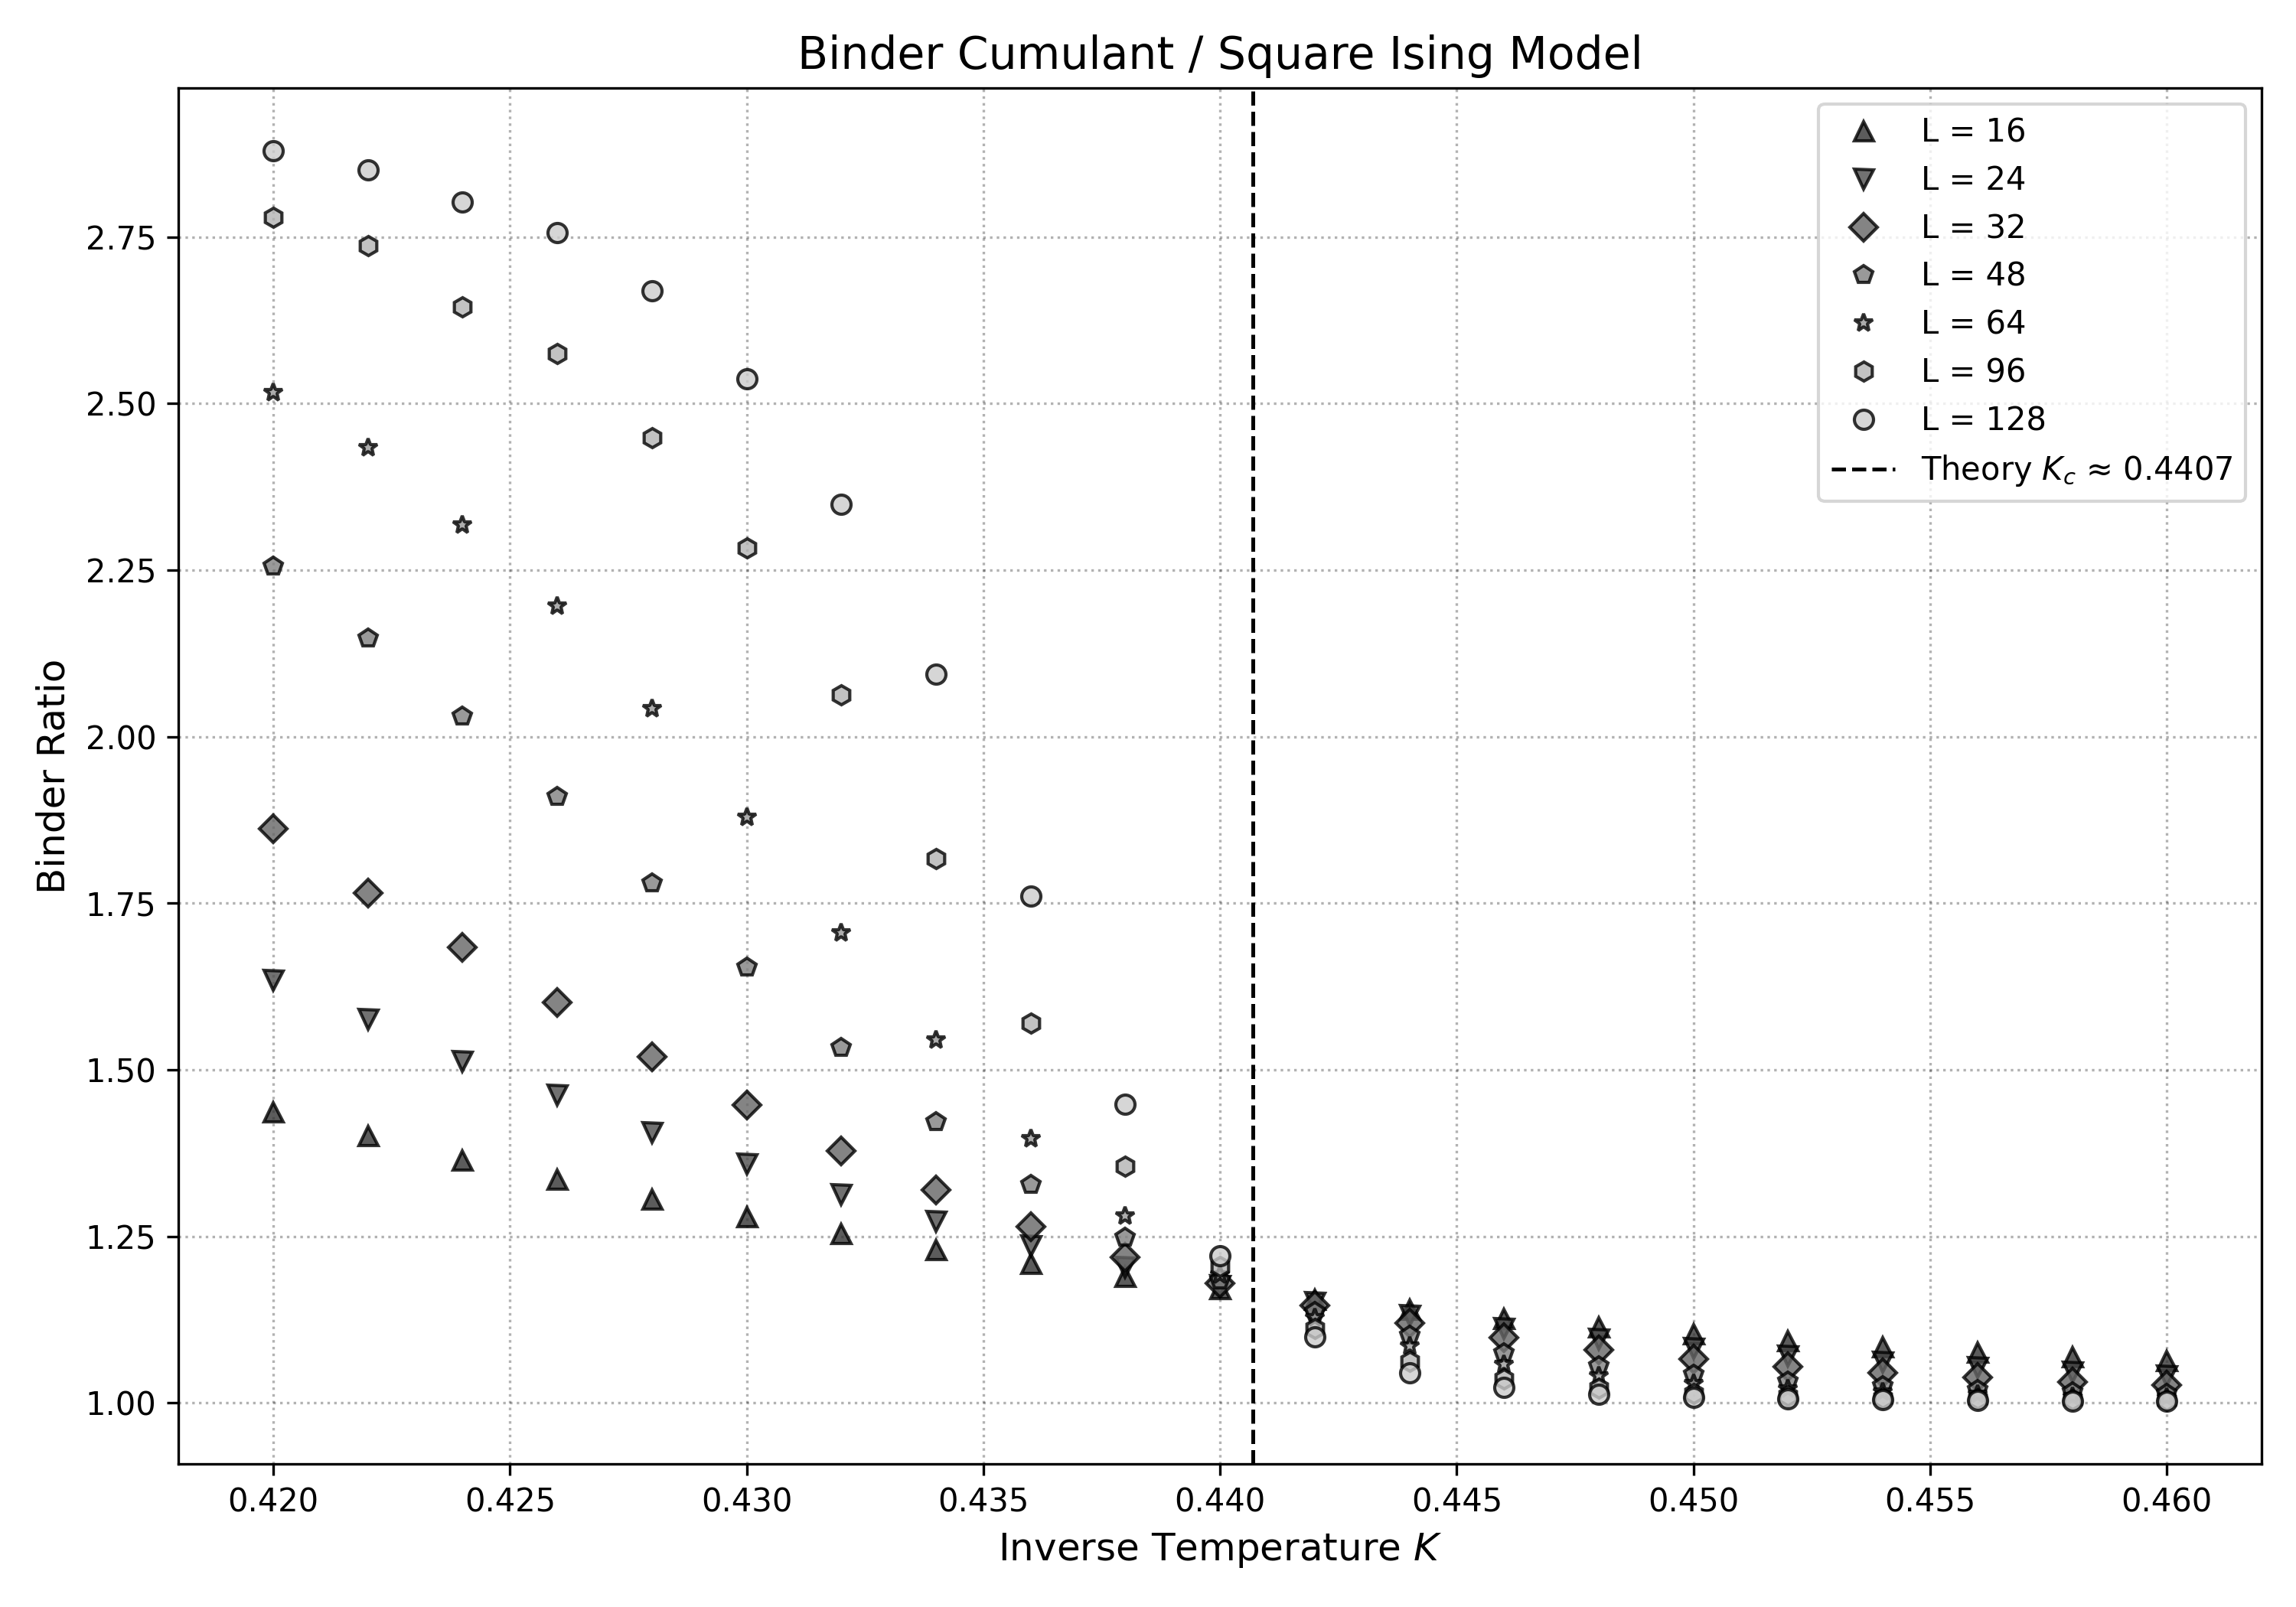
\includegraphics[width=\textwidth]{square_ising_monochrome.png}
  \caption{正方格子上のイジング模型のビンダー比}
  \label{fig:square_ising}
\end{figure}

\umen 全部おなじところで交わってる！
\\\hiron そう。無限に大きい理想的な系ではビンダー比はステップ関数的に変化して、有限の系では系の大きさが大きいほど無限系でのグラフに近づくから、転移温度のところではちょうどすべてのグラフが一点で交わることになる。わかりやすいように、さっき手計算で求めた厳密な転移温度のところに縦線を引いておいた。ビンダー比が転移温度で系の大きさによらない定数になるのは、ふたつの理由によっている。ひとつは、(\ref{eq:binder_ratio})が\textbf{スケールによらない無次元量}になるから。もうひとつは、転移温度でのイジング模型が\textbf{スケール不変}な模型になるから。------実はより強く、このとき系は\textbf{共形不変}な模型になっている。つまり、系のサンプルを1つとってきたときに、スピンの大きな塊も小さな塊も同程度の頻度で観測されるという性質がある。このように、有限サイズの系での数値実験の情報から無限に大きい理想的な系の情報を得る方法を\textbf{有限サイズスケーリング}、およびそれを用いた解析という。有限サイズスケーリングに用いられる観測量はビンダー比だけじゃなくて他にもあって、転移温度以外の系の情報を得ることもできる\footnote{たとえば、このあとの\ref{subsection:triangle_and_honeycomb_lattice_ising}節の最後で話すような臨界指数などが得られる。}から、興味があったら調べてみて、ね。……そろそろ休憩を終わって次の話に行ってもいいかな。
\\\umen うん！　おもしろいグラフも見られたし準備ばっちりだよ！！
\\\chinan わたくしも大丈夫ですわ！
\\\hiron じゃあ、つぎは正方格子じゃない、別の格子の上で考えたらどうなるかについて話そう。

\subsection{三角格子と蜂の巣格子}
\label{subsection:triangle_and_honeycomb_lattice_ising}
\hiron こんどは正方格子じゃなくて、三角格子と蜂の巣格子の上でのイジング模型について考える。三角格子と蜂の巣格子っていうのは、こんな感じの格子。三角格子は文字どおり三角形による平面の敷き詰めになっている。蜂の巣格子は六角形による平面の敷き詰めだけど、``六角格子''とはあまり言わずに、蜂の巣格子って呼ぶ。ちょっとわかりづらいけど、``蜂の巣格子''って呼ぶわりに、六角形の中じゃなくて頂点に変数が棲んでいる、よ。このふたつの格子はこんなふうに、互いに双対格子の関係になっている。さっきまでの正方格子とちがって、自分自身が双対格子になっているわけじゃないから注意して、ね。

\begin{center}
\begin{tikzpicture}[scale=0.95]
  \pgfmathsetmacro{\h}{sqrt(3)/2}

  \node[font=\small] at (1.5,3.2) {三角格子};

  \draw[gray!75, thick] (0,0) -- (3,0);
  \draw[gray!75, thick] (0.5,\h) -- (2.5,\h);
  \draw[gray!75, thick] (0,2*\h) -- (3,2*\h);
  \draw[gray!75, thick] (0.5,3*\h) -- (2.5,3*\h);

  \draw[gray!75, thick] (0,0) -- (1.5,3*\h);
  \draw[gray!75, thick] (1,0) -- (2.5,3*\h);
  \draw[gray!75, thick] (2,0) -- (3,2*\h);
  \draw[gray!75, thick] (0,2*\h) -- (0.5,3*\h);

  \draw[gray!75, thick] (1,0) -- (0,2*\h);
  \draw[gray!75, thick] (2,0) -- (0.5,3*\h);
  \draw[gray!75, thick] (3,0) -- (1.5,3*\h);
  \draw[gray!75, thick] (3,2*\h) -- (2.5,3*\h);

  \foreach \x in {0,1,2,3} {
    \fill[black] (\x,0) circle (1.8pt);
    \fill[black] (\x,2*\h) circle (1.8pt);
  }
  \foreach \x in {0,1,2} {
    \fill[black] (\x+0.5,\h) circle (1.8pt);
    \fill[black] (\x+0.5,3*\h) circle (1.8pt);
  }

  \draw[->, line width=0.9pt] (3.5,1.5) -- (5.8,1.5);
  \node[font=\small, align=center] at (4.65,2.35) {各面の中心に\\対応する頂点};

  \node[font=\small] at (8.0,3.2) {双対格子（蜂の巣格子）};
  \begin{scope}[xshift=6cm]
    \draw[gray!75, thick] (0,0) -- (3,0);
    \draw[gray!75, thick] (0.5,\h) -- (2.5,\h);
    \draw[gray!75, thick] (0,2*\h) -- (3,2*\h);
    \draw[gray!75, thick] (0.5,3*\h) -- (2.5,3*\h);

    \draw[gray!75, thick] (0,0) -- (1.5,3*\h);
    \draw[gray!75, thick] (1,0) -- (2.5,3*\h);
    \draw[gray!75, thick] (2,0) -- (3,2*\h);
    \draw[gray!75, thick] (0,2*\h) -- (0.5,3*\h);

    \draw[gray!75, thick] (1,0) -- (0,2*\h);
    \draw[gray!75, thick] (2,0) -- (0.5,3*\h);
    \draw[gray!75, thick] (3,0) -- (1.5,3*\h);
    \draw[gray!75, thick] (3,2*\h) -- (2.5,3*\h);

    \foreach \x in {1.0, 2.0} {
      \draw[black, dashed] (\x, \h/3*2) -- (\x, \h/3*4);
    }
    \foreach \x in {0.5, 1.5, 2.5} {
      \draw[black, dashed] (\x, \h/3*5) -- (\x, \h/3*7);
    }
    \draw[black, dashed] (0.5, \h/3) -- (1.0, \h/3*2);
    \draw[black, dashed] (1.5, \h/3) -- (2.0, \h/3*2);
    \draw[black, dashed] (1.0, \h/3*4) -- (1.5, \h/3*5);
    \draw[black, dashed] (2.0, \h/3*4) -- (2.5, \h/3*5);
    \draw[black, dashed] (0.5, \h/3*7) -- (1.0, \h/3*8);
    \draw[black, dashed] (1.5, \h/3*7) -- (2.0, \h/3*8);

    \draw[black, dashed] (1.5, \h/3) -- (1.0, \h/3*2);
    \draw[black, dashed] (2.5, \h/3) -- (2.0, \h/3*2);
    \draw[black, dashed] (1.0, \h/3*4) -- (0.5, \h/3*5);
    \draw[black, dashed] (2.0, \h/3*4) -- (1.5, \h/3*5);
    \draw[black, dashed] (1.5, \h/3*7) -- (1.0, \h/3*8);
    \draw[black, dashed] (2.5, \h/3*7) -- (2.0, \h/3*8);

    \foreach \p in {
      (0.5, \h/3), (1.5, \h/3), (2.5, \h/3),
      (1.0, \h/3*2), (2.0, \h/3*2),
      (1.0, \h/3*4), (2.0, \h/3*4),
      (0.5, \h/3*5), (1.5, \h/3*5), (2.5, \h/3*5),
      (0.5, \h/3*7), (1.5, \h/3*7), (2.5, \h/3*7),
      (1.0, \h/3*8), (2.0, \h/3*8)
    } {
      \fill[black] \p circle (1.8pt);
    }
  \end{scope}
  \node[above, align=center, font=\small\bfseries] at (current bounding box.north) {
    三角格子とその双対格子（蜂の巣格子）
  };
\end{tikzpicture}
\end{center}

\begin{comment}
\begin{center}
\begin{tikzpicture}[scale=0.95]
  \pgfmathsetmacro{\h}{sqrt(3)/2}

  \node[font=\small] at (1.5,4.2) {三角格子};

  \draw[gray!65] (0,0) -- (3,0);
  \draw[gray!65] (0.5,\h) -- (2.5,\h);
  \draw[gray!65] (0,2*\h) -- (3,2*\h);
  \draw[gray!65] (0.5,3*\h) -- (2.5,3*\h);

  \draw[gray!65] (0,0) -- (1.5,3*\h);
  \draw[gray!65] (1,0) -- (2.5,3*\h);
  \draw[gray!65] (2,0) -- (3,2*\h);
  \draw[gray!65] (0,2*\h) -- (0.5,3*\h);

  \draw[gray!65] (1,0) -- (0,2*\h);
  \draw[gray!65] (2,0) -- (0.5,3*\h);
  \draw[gray!65] (3,0) -- (1.5,3*\h);
  \draw[gray!65] (3,2*\h) -- (2.5,3*\h);

  \foreach \x in {0,1,2,3} {
    \fill[black] (\x,0) circle (1.8pt);
    \fill[black] (\x,2*\h) circle (1.8pt);
  }
  \foreach \x in {0,1,2} {
    \fill[black] (\x+0.5,\h) circle (1.8pt);
    \fill[black] (\x+0.5,3*\h) circle (1.8pt);
  }

  \draw[->, line width=0.9pt] (3.5,1.5) -- (5.8,1.5);
  \node[font=\small, align=center] at (4.65,2.35) {各面の中心に\\対応する頂点};

  \node[font=\small] at (8.0,4.2) {双対格子（蜂の巣格子）};
  \begin{scope}[xshift=6cm]
    \draw[gray!35] (0,0) -- (3,0);
    \draw[gray!35] (0.5,\h) -- (2.5,\h);
    \draw[gray!35] (0,2*\h) -- (3,2*\h);
    \draw[gray!35] (0.5,3*\h) -- (2.5,3*\h);

    \draw[gray!35] (0,0) -- (1.5,3*\h);
    \draw[gray!35] (1,0) -- (2.5,3*\h);
    \draw[gray!35] (2,0) -- (3,2*\h);
    \draw[gray!35] (0,2*\h) -- (0.5,3*\h);

    \draw[gray!35] (1,0) -- (0,2*\h);
    \draw[gray!35] (2,0) -- (0.5,3*\h);
    \draw[gray!35] (3,0) -- (1.5,3*\h);
    \draw[gray!35] (3,2*\h) -- (2.5,3*\h);

    \foreach \x in {1.0, 2.0} {
      \draw[red!80, dashed] (\x, \h/3*2) -- (\x, \h/3*4);
    }
    \foreach \x in {0.5, 1.5, 2.5} {
      \draw[red!80, dashed] (\x, \h/3*5) -- (\x, \h/3*7);
    }
    \draw[red!80, dashed] (0.5, \h/3) -- (1.0, \h/3*2);
    \draw[red!80, dashed] (1.5, \h/3) -- (2.0, \h/3*2);
    \draw[red!80, dashed] (1.0, \h/3*4) -- (1.5, \h/3*5);
    \draw[red!80, dashed] (2.0, \h/3*4) -- (2.5, \h/3*5);
    \draw[red!80, dashed] (0.5, \h/3*7) -- (1.0, \h/3*8);
    \draw[red!80, dashed] (1.5, \h/3*7) -- (2.0, \h/3*8);

    \draw[red!80, dashed] (1.5, \h/3) -- (1.0, \h/3*2);
    \draw[red!80, dashed] (2.5, \h/3) -- (2.0, \h/3*2);
    \draw[red!80, dashed] (1.0, \h/3*4) -- (0.5, \h/3*5);
    \draw[red!80, dashed] (2.0, \h/3*4) -- (1.5, \h/3*5);
    \draw[red!80, dashed] (1.5, \h/3*7) -- (1.0, \h/3*8);
    \draw[red!80, dashed] (2.5, \h/3*7) -- (2.0, \h/3*8);

    \foreach \p in {
      (0.5, \h/3), (1.5, \h/3), (2.5, \h/3),
      (1.0, \h/3*2), (2.0, \h/3*2),
      (1.0, \h/3*4), (2.0, \h/3*4),
      (0.5, \h/3*5), (1.5, \h/3*5), (2.5, \h/3*5),
      (0.5, \h/3*7), (1.5, \h/3*7), (2.5, \h/3*7),
      (1.0, \h/3*8), (2.0, \h/3*8)
    } {
      \fill[red!80] \p circle (1.8pt);
    }
  \end{scope}
  \node[above, align=center, font=\small\bfseries] at (current bounding box.north) {
    三角格子とその双対格子（蜂の巣格子）
  };
\end{tikzpicture}
\end{center}
\end{comment}

この格子の上でのイジング模型の厳密な転移温度を正方格子のときとおなじように求めてみよう。実は、(\ref{eq:distribution_function_ising})からスタートしてまったくおなじ計算をたどることで、(\ref{eq:dual_temperature_ising})にあたる、
\begin{align}
  \coth K_{\mathrm{triangle}}=\exp\left(2K^\ast_{\mathrm{honeycomb}}\right),\label{eq:dual_temperature_ising_triangle_honeycomb}
\end{align}
が得られる。正方格子では1つのサイトに対して隣接するサイトが4つだから(\ref{eq:FT_site_expression})-(\ref{eq:distribution_function_ising_bond_sum})にでてくる$s_{ia}+s_{ib}-s_{ic}-s_{id}$の部分は項が4つだったけど、三角格子のときは隣接サイトが6つあるから項も6つになるところだけが変わるから注意して、ね\footnote{もちろんここの詳細が気になるなら演習問題だ、よ。}。こんどは双対格子が自分自身とおなじ格子になっていないから、(\ref{eq:dual_temperature_ising_triangle_honeycomb})から直接は転移温度を求めることができない。そこで\textbf{star-triangle変換}、または\textbf{Y-$\Delta$変換}と呼ばれるうまいトリックを使う。こんなふうに、双対変換後の蜂の巣格子で1つおきにサイトを抜き出した副格子の上で、スピンの状態について和をとってしまう。そうすると残った格子はもとの格子とおなじ形の三角格子になって、分配関数も三角格子のイジング模型のものになるから温度の比較ができるようになる。

\begin{center}
\begin{tikzpicture}[scale=0.95]
  % 単位ベクトルの成分（計算用）
  \pgfmathsetmacro{\dx}{1.73205} % sqrt(3)
  \pgfmathsetmacro{\dy}{1.5}

  % ==========================================
  % 左側：蜂の巣格子（2つの副格子）
  % ==========================================
  \node[font=\small] at (1.5,4.3) {蜂の巣格子};
  \node[font=\footnotesize] at (1.5,3.9) {（黒丸：副格子A，白丸：副格子B）};

  \begin{scope}
    % 描画領域をクリップして端を綺麗に揃える
    \clip (-0.5, -0.2) rectangle (3.7, 3.6);

    % 蜂の巣格子の線
    \foreach \m in {-2,-1,0,1,2,3} {
      \foreach \n in {-2,-1,0,1,2,3} {
        \pgfmathsetmacro{\Ax}{\m*\dx + \n*\dx/2}
        \pgfmathsetmacro{\Ay}{\n*\dy}
        \pgfmathsetmacro{\Bx}{\Ax}
        \pgfmathsetmacro{\By}{\Ay + 1.0}
        \pgfmathsetmacro{\BdnLx}{\m*\dx + (\n-1)*\dx/2}
        \pgfmathsetmacro{\BdnLy}{(\n-1)*\dy + 1.0}
        \pgfmathsetmacro{\BdnRx}{(\m+1)*\dx + (\n-1)*\dx/2}
        \pgfmathsetmacro{\BdnRy}{(\n-1)*\dy + 1.0}

        \draw[gray!75, thick] (\Ax, \Ay) -- (\Bx, \By);
        \draw[gray!75, thick] (\Ax, \Ay) -- (\BdnLx, \BdnLy);
        \draw[gray!75, thick] (\Ax, \Ay) -- (\BdnRx, \BdnRy);
      }
    }

    % 頂点（A=黒, B=白）
    \foreach \m in {-2,-1,0,1,2,3} {
      \foreach \n in {-2,-1,0,1,2,3} {
        \pgfmathsetmacro{\Ax}{\m*\dx + \n*\dx/2}
        \pgfmathsetmacro{\Ay}{\n*\dy}
        \pgfmathsetmacro{\Bx}{\Ax}
        \pgfmathsetmacro{\By}{\Ay + 1.0}

        % 副格子A
        \fill[black] (\Ax, \Ay) circle (2.2pt);
        % 副格子B
        \fill[white] (\Bx, \By) circle (2.2pt);
        \draw[black, thick] (\Bx, \By) circle (2.2pt);
      }
    }
  \end{scope}

  % ==========================================
  % 中央の矢印と説明テキスト
  % ==========================================
  \draw[->, line width=0.9pt] (4.3,1.8) -- (7.5,1.8);
  \node[font=\small, align=center] at (6.0,2.9) {副格子B(白丸)の\\部分和をとる\\(トレース)};

  % ==========================================
  % 右側：三角格子（変換後）
  % ==========================================
  \node[font=\small] at (10.4,4.3) {三角格子};
  \node[font=\footnotesize] at (10.4,3.9) {（有効相互作用）};

  \begin{scope}[xshift=9.0cm]
    \clip (-0.5, -0.2) rectangle (3.7, 3.6);

    % 薄い蜂の巣格子（消去された元の格子）
    \foreach \m in {-2,-1,0,1,2,3} {
      \foreach \n in {-2,-1,0,1,2,3} {
        \pgfmathsetmacro{\Ax}{\m*\dx + \n*\dx/2}
        \pgfmathsetmacro{\Ay}{\n*\dy}
        \pgfmathsetmacro{\Bx}{\Ax}
        \pgfmathsetmacro{\By}{\Ay + 1.0}
        \pgfmathsetmacro{\BdnLx}{\m*\dx + (\n-1)*\dx/2}
        \pgfmathsetmacro{\BdnLy}{(\n-1)*\dy + 1.0}
        \pgfmathsetmacro{\BdnRx}{(\m+1)*\dx + (\n-1)*\dx/2}
        \pgfmathsetmacro{\BdnRy}{(\n-1)*\dy + 1.0}

        \draw[gray!75, thick] (\Ax, \Ay) -- (\Bx, \By);
        \draw[gray!75, thick] (\Ax, \Ay) -- (\BdnLx, \BdnLy);
        \draw[gray!75, thick] (\Ax, \Ay) -- (\BdnRx, \BdnRy);
      }
    }

    % 三角格子の線（青色破線で新たな有効相互作用を表現）
    \foreach \m in {-2,-1,0,1,2,3} {
      \foreach \n in {-2,-1,0,1,2,3} {
        \pgfmathsetmacro{\Ax}{\m*\dx + \n*\dx/2}
        \pgfmathsetmacro{\Ay}{\n*\dy}
        
        \pgfmathsetmacro{\AoneX}{(\m+1)*\dx + \n*\dx/2}
        \pgfmathsetmacro{\AoneY}{\n*\dy}
        \pgfmathsetmacro{\AtwoX}{\m*\dx + (\n+1)*\dx/2}
        \pgfmathsetmacro{\AtwoY}{(\n+1)*\dy}
        \pgfmathsetmacro{\AthreeX}{(\m-1)*\dx + (\n+1)*\dx/2}
        \pgfmathsetmacro{\AthreeY}{(\n+1)*\dy}

        \draw[black, thick, dashed] (\Ax, \Ay) -- (\AoneX, \AoneY);
        \draw[black, thick, dashed] (\Ax, \Ay) -- (\AtwoX, \AtwoY);
        \draw[black, thick, dashed] (\Ax, \Ay) -- (\AthreeX, \AthreeY);
      }
    }

    % 頂点（残った副格子Aのみを明示）
    \foreach \m in {-2,-1,0,1,2,3} {
      \foreach \n in {-2,-1,0,1,2,3} {
        \pgfmathsetmacro{\Ax}{\m*\dx + \n*\dx/2}
        \pgfmathsetmacro{\Ay}{\n*\dy}
        \fill[black] (\Ax, \Ay) circle (2.2pt);
      }
    }
  \end{scope}
  \node[above, align=center, font=\small\bfseries] at (current bounding box.north) {
    蜂の巣格子から三角格子へのstar-triangle変換
  };
\end{tikzpicture}
\end{center}

\begin{comment}
\begin{center}
\begin{tikzpicture}[scale=0.95]
  % 単位ベクトルの成分（計算用）
  \pgfmathsetmacro{\dx}{1.73205} % sqrt(3)
  \pgfmathsetmacro{\dy}{1.5}

  % ==========================================
  % 左側：蜂の巣格子（2つの副格子）
  % ==========================================
  \node[font=\small] at (1.5,4.3) {蜂の巣格子};
  \node[font=\footnotesize, gray] at (1.5,3.9) {（黒丸：副格子A，白丸：副格子B）};

  \begin{scope}
    % 描画領域をクリップして端を綺麗に揃える
    \clip (-0.5, -0.2) rectangle (3.7, 3.6);

    % 蜂の巣格子の線
    \foreach \m in {-2,-1,0,1,2,3} {
      \foreach \n in {-2,-1,0,1,2,3} {
        \pgfmathsetmacro{\Ax}{\m*\dx + \n*\dx/2}
        \pgfmathsetmacro{\Ay}{\n*\dy}
        \pgfmathsetmacro{\Bx}{\Ax}
        \pgfmathsetmacro{\By}{\Ay + 1.0}
        \pgfmathsetmacro{\BdnLx}{\m*\dx + (\n-1)*\dx/2}
        \pgfmathsetmacro{\BdnLy}{(\n-1)*\dy + 1.0}
        \pgfmathsetmacro{\BdnRx}{(\m+1)*\dx + (\n-1)*\dx/2}
        \pgfmathsetmacro{\BdnRy}{(\n-1)*\dy + 1.0}

        \draw[gray!65, thick] (\Ax, \Ay) -- (\Bx, \By);
        \draw[gray!65, thick] (\Ax, \Ay) -- (\BdnLx, \BdnLy);
        \draw[gray!65, thick] (\Ax, \Ay) -- (\BdnRx, \BdnRy);
      }
    }

    % 頂点（A=黒, B=白）
    \foreach \m in {-2,-1,0,1,2,3} {
      \foreach \n in {-2,-1,0,1,2,3} {
        \pgfmathsetmacro{\Ax}{\m*\dx + \n*\dx/2}
        \pgfmathsetmacro{\Ay}{\n*\dy}
        \pgfmathsetmacro{\Bx}{\Ax}
        \pgfmathsetmacro{\By}{\Ay + 1.0}

        % 副格子A
        \fill[black] (\Ax, \Ay) circle (2.2pt);
        % 副格子B
        \fill[white] (\Bx, \By) circle (2.2pt);
        \draw[black, thick] (\Bx, \By) circle (2.2pt);
      }
    }
  \end{scope}

  % ==========================================
  % 中央の矢印と説明テキスト
  % ==========================================
  \draw[->, line width=0.9pt] (4.3,1.8) -- (7.5,1.8);
  \node[font=\small, align=center] at (6.0,2.9) {副格子B(白丸)の\\部分和をとる\\(トレース)};

  % ==========================================
  % 右側：三角格子（変換後）
  % ==========================================
  \node[font=\small] at (10.4,4.3) {三角格子};
  \node[font=\footnotesize, gray] at (10.4,3.9) {（有効相互作用）};

  \begin{scope}[xshift=9.0cm]
    \clip (-0.5, -0.2) rectangle (3.7, 3.6);

    % 薄い蜂の巣格子（消去された元の格子）
    \foreach \m in {-2,-1,0,1,2,3} {
      \foreach \n in {-2,-1,0,1,2,3} {
        \pgfmathsetmacro{\Ax}{\m*\dx + \n*\dx/2}
        \pgfmathsetmacro{\Ay}{\n*\dy}
        \pgfmathsetmacro{\Bx}{\Ax}
        \pgfmathsetmacro{\By}{\Ay + 1.0}
        \pgfmathsetmacro{\BdnLx}{\m*\dx + (\n-1)*\dx/2}
        \pgfmathsetmacro{\BdnLy}{(\n-1)*\dy + 1.0}
        \pgfmathsetmacro{\BdnRx}{(\m+1)*\dx + (\n-1)*\dx/2}
        \pgfmathsetmacro{\BdnRy}{(\n-1)*\dy + 1.0}

        \draw[gray!20, thick] (\Ax, \Ay) -- (\Bx, \By);
        \draw[gray!20, thick] (\Ax, \Ay) -- (\BdnLx, \BdnLy);
        \draw[gray!20, thick] (\Ax, \Ay) -- (\BdnRx, \BdnRy);
      }
    }

    % 三角格子の線（青色破線で新たな有効相互作用を表現）
    \foreach \m in {-2,-1,0,1,2,3} {
      \foreach \n in {-2,-1,0,1,2,3} {
        \pgfmathsetmacro{\Ax}{\m*\dx + \n*\dx/2}
        \pgfmathsetmacro{\Ay}{\n*\dy}
        
        \pgfmathsetmacro{\AoneX}{(\m+1)*\dx + \n*\dx/2}
        \pgfmathsetmacro{\AoneY}{\n*\dy}
        \pgfmathsetmacro{\AtwoX}{\m*\dx + (\n+1)*\dx/2}
        \pgfmathsetmacro{\AtwoY}{(\n+1)*\dy}
        \pgfmathsetmacro{\AthreeX}{(\m-1)*\dx + (\n+1)*\dx/2}
        \pgfmathsetmacro{\AthreeY}{(\n+1)*\dy}

        \draw[blue!70, thick, dashed] (\Ax, \Ay) -- (\AoneX, \AoneY);
        \draw[blue!70, thick, dashed] (\Ax, \Ay) -- (\AtwoX, \AtwoY);
        \draw[blue!70, thick, dashed] (\Ax, \Ay) -- (\AthreeX, \AthreeY);
      }
    }

    % 頂点（残った副格子Aのみを明示）
    \foreach \m in {-2,-1,0,1,2,3} {
      \foreach \n in {-2,-1,0,1,2,3} {
        \pgfmathsetmacro{\Ax}{\m*\dx + \n*\dx/2}
        \pgfmathsetmacro{\Ay}{\n*\dy}
        \fill[black] (\Ax, \Ay) circle (2.2pt);
      }
    }
  \end{scope}
  \node[above, align=center, font=\small\bfseries] at (current bounding box.north) {
    蜂の巣格子から三角格子へのstar-triangle変換
  };
\end{tikzpicture}
\end{center}
\end{comment}

\begin{center}
\begin{tikzpicture}[scale=1.05]
  % 左: triangle (Δ)
  \node[font=\small] at (0.2,2.45) {Star (Y) 側};
  \coordinate (A2) at (-0.8,0);
  \coordinate (B2) at (1.2,0);
  \coordinate (C2) at (0.2,1.7);
  \coordinate (O)  at (0.2,0.7);
  \fill (A2) circle (2.2pt) node[below left=2pt] {$\sigma_1$};
  \fill (B2) circle (2.2pt) node[below right=2pt] {$\sigma_2$};
  \fill (C2) circle (2.2pt) node[above=2pt] {$\sigma_3$};
  \fill (O)  circle (2.2pt) node[right=2pt] {$\sigma$};
  \draw[line width=0.9pt] (O) -- node[pos=0.58, above left=1pt, xshift=10pt, yshift=-2pt] {$K^\ast$} (A2);
  \draw[line width=0.9pt] (O) -- node[pos=0.58, right=1pt, xshift=-5pt, yshift=7pt] {$K^\ast$} (B2);
  \draw[line width=0.9pt] (O) -- node[right=0pt] {$K^\ast$} (C2);

  % 変換矢印
  \draw[->, line width=1.0pt] (2.0,0.85) -- (4.2,0.85)
    node[midway, above=3pt] {star-triangle 変換};

  % 右: star (Y)
  \node[font=\small] at (6,2.45) {Triangle ($\Delta$) 側};
  \coordinate (A) at (5,0);
  \coordinate (B) at (7,0);
  \coordinate (C) at (6,1.7);
  \fill (A) circle (2.2pt) node[below left=2pt] {$\sigma_1$};
  \fill (B) circle (2.2pt) node[below right=2pt] {$\sigma_2$};
  \fill (C) circle (2.2pt) node[above=2pt] {$\sigma_3$};
  \draw[line width=0.9pt] (A) -- node[below=2pt] {$\tilde K$} (B);
  \draw[line width=0.9pt] (B) -- node[right=2pt] {$\tilde K$} (C);
  \draw[line width=0.9pt] (C) -- node[left=2pt] {$\tilde K$} (A);

  \node[font=\small, align=center] at (3.1,-1.0)
    {$\sum_{\sigma=\pm1} \exp\left[K^\ast\sigma(\sigma_1+\sigma_2+\sigma_3)\right]
    \propto \exp\left[\tilde K(\sigma_1\sigma_2+\sigma_2\sigma_3+\sigma_3\sigma_1)\right]$};
\end{tikzpicture}
\end{center}

新しい三角格子の逆温度を$\tilde K$とすると、
\begin{align}
  \sum_{\sigma=\pm1}\exp[K^\ast\sigma(\sigma_1+\sigma_2+\sigma_3)]=A(K)\exp[\tilde K(\sigma_1\sigma_2+\sigma_2\sigma_3+\sigma_3\sigma_1)],\label{eq:star-triangle_eq}
\end{align}
であればいい。これは、
\begin{align}
  \begin{cases}
    2\cosh(3K^\ast)&=A(K)\exp(3\tilde K)\\
    2\cosh K^\ast&=A(K)\exp(-\tilde K)
  \end{cases},
\end{align}
とおなじだから、これを解いて、
\begin{align}
  \exp(4\tilde K)=\frac{\cosh(3K^\ast)}{\cosh K^\ast}.\label{eq:temperature_relation_star_triangle}
\end{align}
ただし、さっきの正方格子のときに議論した話とおなじで、状態によらない定数を分配関数全体にかけることになるだけだから$A(K)$の中身は気にしなくていい。(\ref{eq:temperature_relation_star_triangle})に(\ref{eq:dual_temperature_ising_triangle_honeycomb})を代入して対称な形に整理すると、
\begin{align}
  [\exp(4K_{\mathrm{triangle}})-1][\exp(4\tilde K_{\mathrm{triangle}})-1]=4.
\end{align}
正方格子のときとおなじ理由で、転移温度$K_{\mathrm{c,triangle}}$は、
\begin{align}
  K_{\mathrm{c,triangle}}=K_{\mathrm{triangle}}=\tilde K_{\mathrm{triangle}},
\end{align}
をみたさないといけない。つまり、
\begin{tcolorbox}
\begin{align}
  K_{\mathrm{c,triangle}}=\frac14\log3,\label{eq:critical_temperature_ising_triangle}
\end{align}
\end{tcolorbox}
がわかった。蜂の巣格子の転移温度は、(\ref{eq:dual_temperature_ising_triangle_honeycomb})に(\ref{eq:critical_temperature_ising_triangle})を代入して整理すると、
\begin{tcolorbox}
\begin{align}
  K_{\mathrm{c,honeycomb}}=\frac12\log\left(2+\sqrt 3\right),\label{eq:critical_temperature_ising_honeycomb}
\end{align}
\end{tcolorbox}
と求まる。

正方格子のときとおなじようにモンテカルロシミュレーションで数値実験した結果があるから見ておこう。

\begin{figure}[H]
  \centering
  % width=\textwidth でページ幅に合わせる
  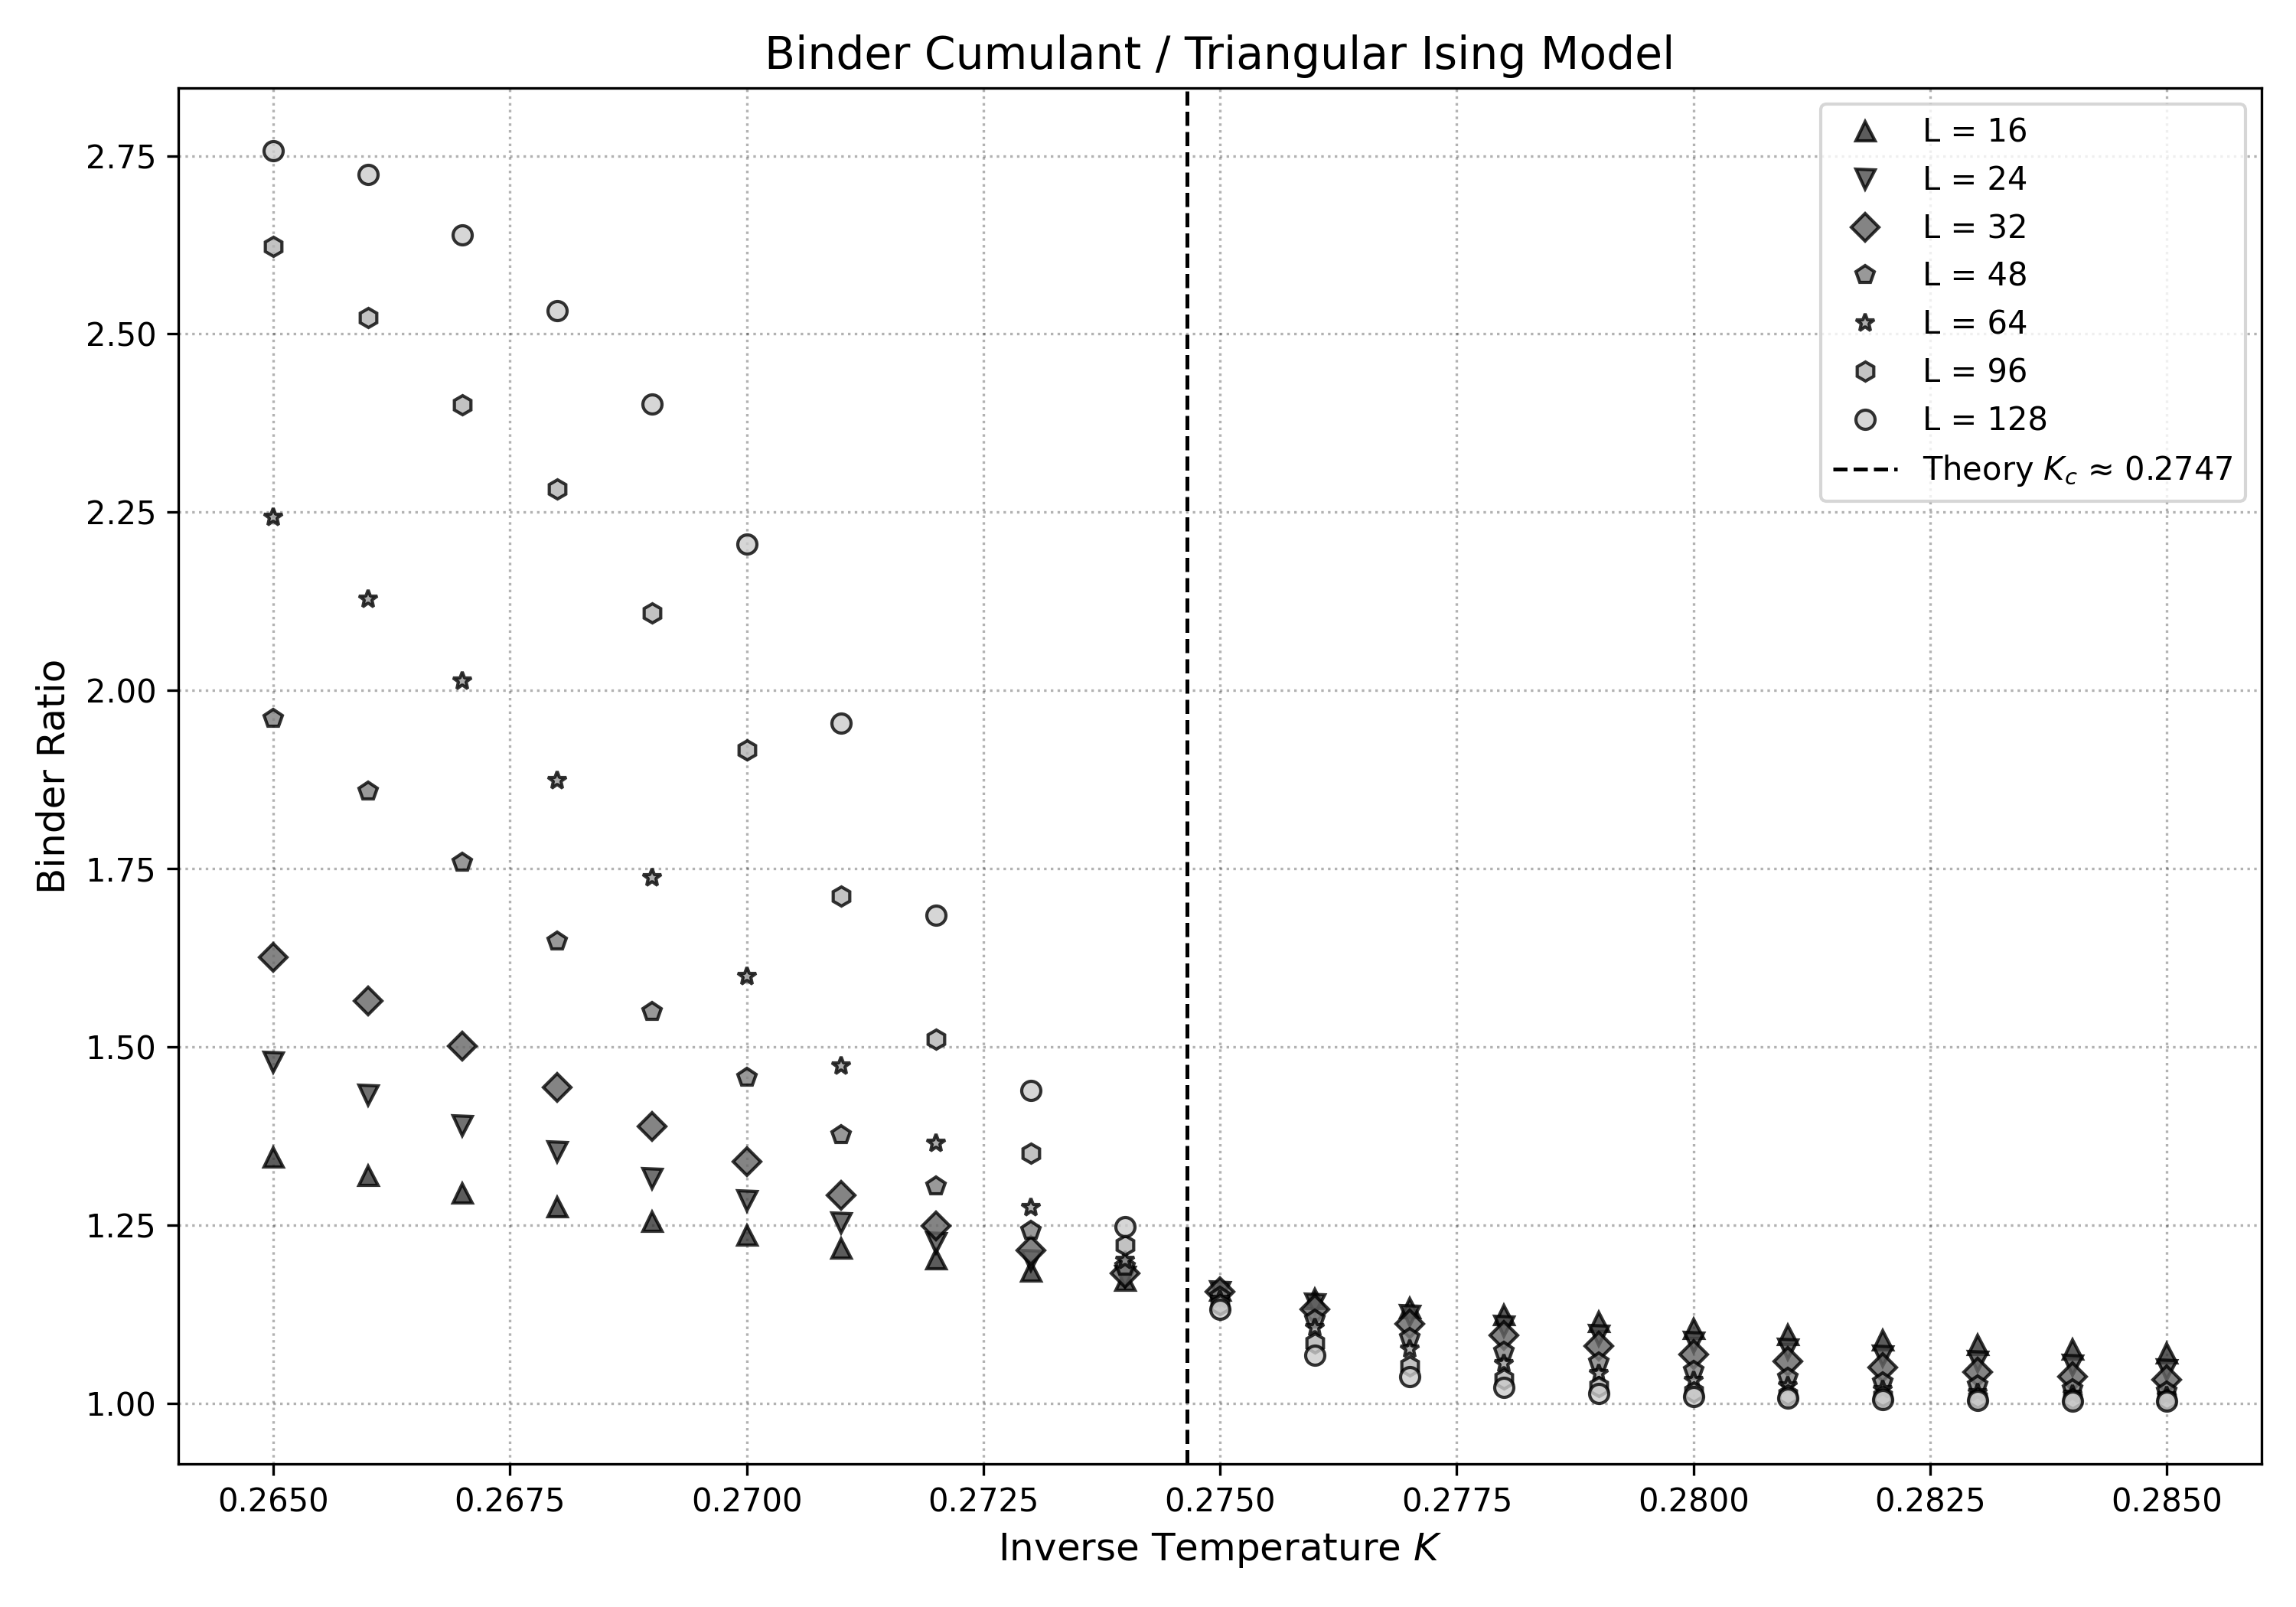
\includegraphics[width=\textwidth]{triangular_ising_monochrome.png}
  \caption{三角格子上のイジング模型のビンダー比}
  \label{fig:triangular_ising}
\end{figure}
\begin{figure}[H]
  \centering
  % width=\textwidth でページ幅に合わせる
  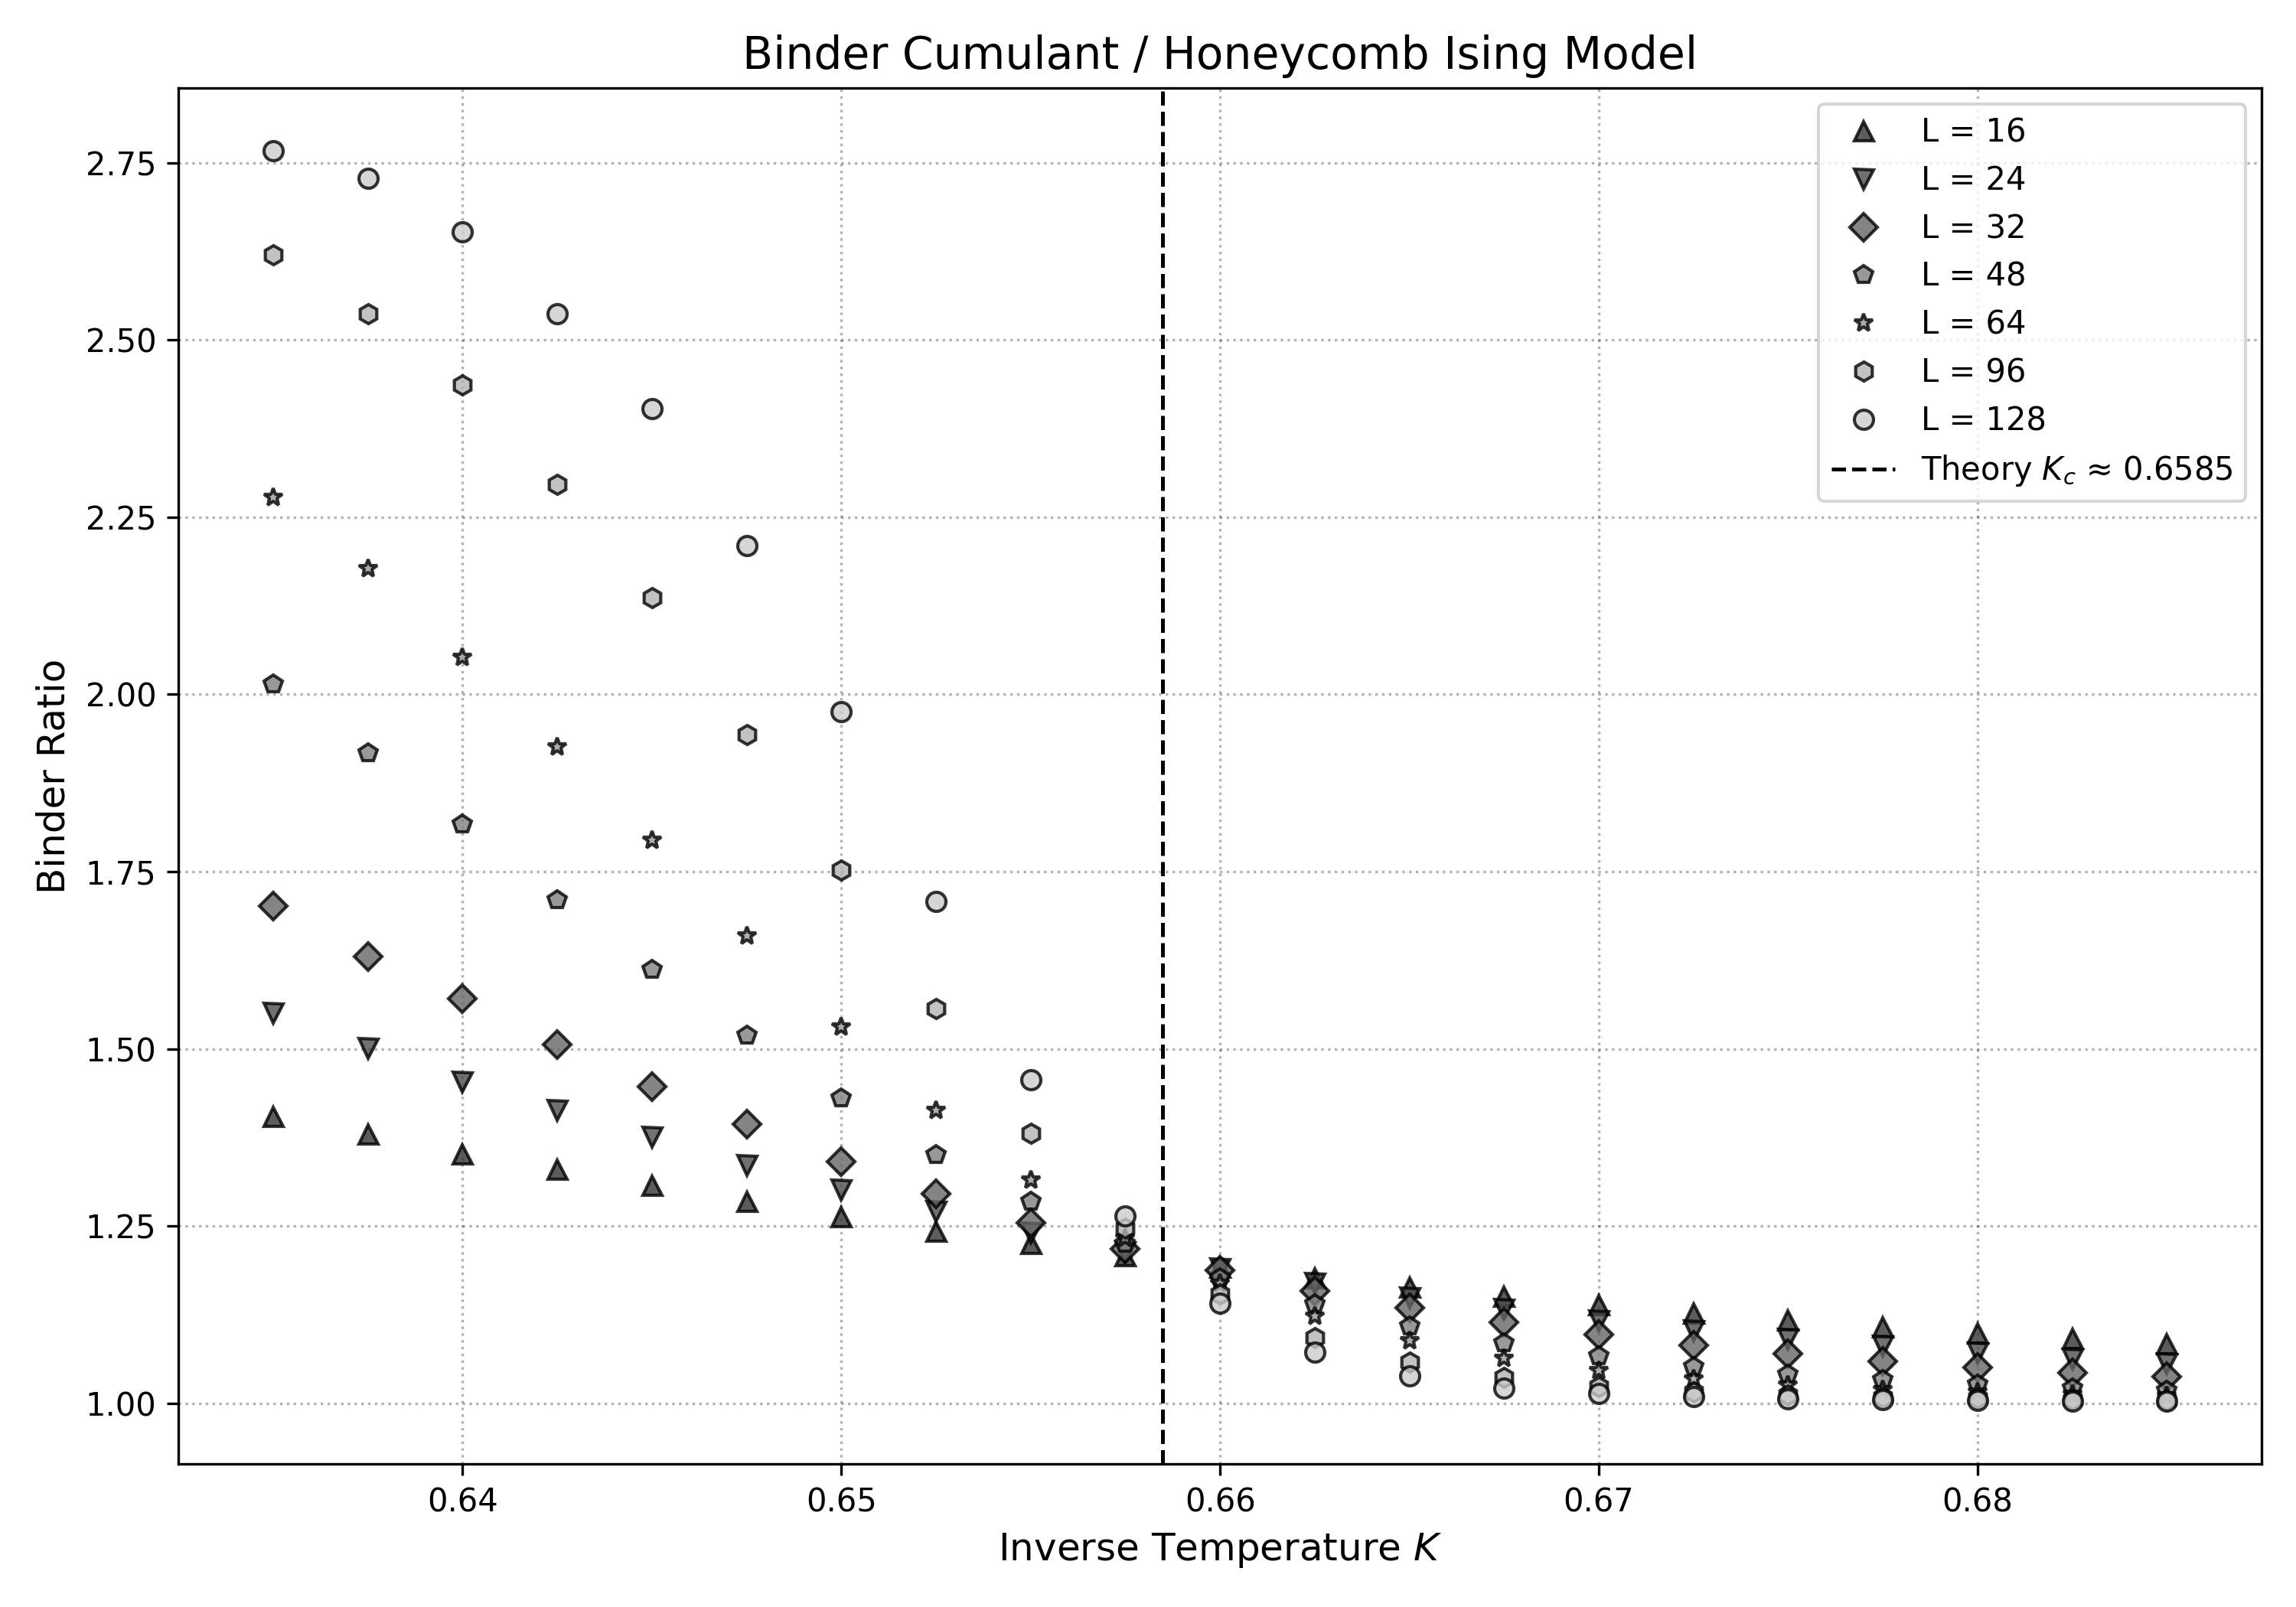
\includegraphics[width=\textwidth]{honeycomb_ising_monochrome.png}
  \caption{蜂の巣格子上のイジング模型のビンダー比}
  \label{fig:honeycomb_ising}
\end{figure}

格子の種類を変えてもビンダー比のグラフはちゃんと転移点で交わることがわかる。

ちなみに、(\ref{eq:spontaneous_magnetisation_2d_square_ising})では自発磁化は転移温度付近で
\begin{align}
  \langle |M|\rangle\sim(K-K_{\mathrm c})^{1/8},
\end{align}
という立ち上がり方をしていたけど、この肩に乗っている指数1/8のことを\textbf{臨界指数}という。臨界指数は自発磁化以外の物理量に対しても定義されるけど、今日の話では詳しく紹介しないから興味があったら調べてみて、ね。実は、2次元イジング模型の臨界指数は、格子が正方格子、三角格子、蜂の巣格子のどれであってもおなじ値になる。それどころか、この3つ以外のもっと複雑な格子を考えてもそれが2次元なら臨界指数はおなじ値になる。この性質を\textbf{ユニバーサリティ}、もしくは\textbf{普遍性}という。臨界指数がおなじになる模型のクラスを\textbf{ユニバーサリティクラス}と呼ぶ。つまり、2次元イジング模型は格子の種類によらずおなじユニバーサリティクラスに属する。これは、格子のサイズを大きくする極限においては格子のミクロな構造が無視されて、格子のマクロな対称性だけが臨界指数の値に効いてくることの現れになっている。もちろん、さっき求めた転移温度は格子のミクロな構造の影響を受けるから、格子によって変わってくる。

ところで、さっき「イジング模型は2次元以下では分配関数や磁化も込みで厳密に解けて、3次元以上では厳密には解けない」って話した。でも実は、4次元以上だと完全には解けないけどある値が厳密に求まる。なんだと思う？
\\\umen 転移温度は厳密に求まる、とか？
\\\hiron 残念だけど不正解。世の中、そんなに甘くない。
\\\chinan ままならない、ですわね$\heartsuit$
\\\umen またふたりでイチャイチャしてる……。
\\\hiron ふふふ……。正解は、「\textbf{4次元以上のイジング模型は臨界指数が厳密に求まる}」。これはどういうことかというと、平均場近似という手法を使う。平均場近似というのは、あるスピンの相互作用相手が、系全体の平均的な値をとる仮想的なスピンだと仮定して計算を進める手法のこと。これはしょせんは近似に過ぎないから、普通は厳密な値は得られない。でも4次元以上ではそもそも相互作用する相手になるスピンの数がじゅうぶん多いから、平均場近似が近似ではなくなって、少なくとも臨界指数に関しては厳密な値を計算することができる。各次元のイジング模型の臨界指数を表にしてまとめておこう。

\begin{center}
\begin{tabular}{c||c|c|c|c|c|c}
  \hline
   & $\alpha$ & $\beta$ & $\gamma$ & $\delta$ & $\eta$ & $\nu$ \\
  \hline\hline
  2D Ising & 0 ($\log$) & $1/8$ & $7/4$ & 15 & $1/4$ & 1 \\
  \hline
  3D Ising & 約0.11 & 約0.326 & 約1.24 & 約4.79 & 約0.036 & 約0.630 \\
  \hline
  $\ge$4D Ising (平均場) & 0 & $1/2$ & 1 & 3 & 0 & $1/2$ \\
  \hline
\end{tabular}
\end{center}

もちろん3次元の結果は数値計算によるもの。ここで各臨界指数のだいたいの意味は、
\begin{itemize}
  \item $\alpha$は比熱、
  \item $\beta$は自発磁化、
  \item $\gamma$は帯磁率、
  \item $\delta$は転移温度上での磁場に対する磁化の立ち上がり、
  \item $\eta$は相関関数の異常次元、
  \item $\nu$は相関長、
\end{itemize}
に関する指数だ、よ。

すこし寄り道もしちゃったけど、これで三角格子や蜂の巣格子でのイジング模型についての理解を深めることができた。つぎはイジング模型そのものの拡張について考えてみよう。

\subsection{ポッツ模型}
\hiron こんどはポッツ模型というのを考えてみよう。\textbf{$\bm q$-状態ポッツ模型}というのはエネルギーが
\begin{align}
  E\{\sigma\}=-J\sum_{(ij)}\delta(\sigma_i,\sigma_j),\quad \sigma_i\in\{0,\dots,q-1\},
\end{align}
で与えられる模型のこと。これは各サイトの状態の数が$q$個に増えていて、隣り合うスピンの状態がおなじときだけエネルギーが低いから、サイトの状態が2つだったイジング模型の自然な拡張になっている。もちろん$q=2$とすればイジング模型に帰着する。ただし、隣り合うスピンがおなじときとちがうときのエネルギーの差の定義が2倍だけずれていることに注意して、ね。この模型でもイジング模型とほぼおなじ方法で、厳密な転移温度を求めることができる。さっきの(\ref{eq:distribution_function_ising})とおなじように、分配関数
\begin{align}
  Z=\sum_{\{\sigma\}}\prod_{(ij)}\exp\left[K\delta(\sigma_i,\sigma_j)\right],\label{eq:distribution_function_potts}
\end{align}
からスタートしよう。ここで種明かしをすると、実は(\ref{eq:FT_interaction_ising})はフーリエ変換をしている。こんどは状態が$q$個あるから、
\begin{align}
  \exp\left[K\delta(\sigma_i,\sigma_j)\right]=\frac1q\sum_{s_{ij}=0}^{q-1}\left[q\delta(s_{ij},0)+e^K-1\right]\exp\left[\frac{2\pi\sqrt{-1}}{q}s_{ij}(\sigma_i-\sigma_j)\right],
\end{align}
というフーリエ変換をすればいい。(\ref{eq:distribution_function_potts})に代入すると、
\begin{align}
  Z=\sum_{\{\sigma\}}\prod_{(ij)}\left(\frac1q\sum_{s_{ij}=0}^{q-1}\left[q\delta(s_{ij},0)+e^K-1\right]\exp\left[\frac{2\pi\sqrt{-1}}{q}s_{ij}(\sigma_i-\sigma_j)\right]\right),
\end{align}
になる。(\ref{eq:FT_bond_expression})から(\ref{eq:distribution_function_ising_dual})を導いたときのように、和の順序を入れ替えて双対格子での分配関数に書き直すと、
\begin{align}
  Z=\sum_{\{\mu\}}\prod_{(ij)}\left[q\delta(\mu_i,\mu_j)+e^K-1\right],
\end{align}
が得られる。これはもとの格子と双対格子の温度のあいだに、
\begin{align}
  \exp(K^\ast)=\frac{e^K+q-1}{e^K-1},\label{eq:dual_temperature_potts}
\end{align}
の関係があることを表している。正方格子の場合はイジング模型の場合とおなじように、$K_{\mathrm{c,square}}=K=K^\ast$が必要だから、(\ref{eq:dual_temperature_potts})からただちに
\begin{tcolorbox}
\begin{align}
  K_{\mathrm{c,square}}=\log\left(1+\sqrt q\right),\label{eq:critical_temperature_potts_square}
\end{align}
\end{tcolorbox}
がわかる。いっぽう、三角格子と蜂の巣格子の場合はすこし難しい。(\ref{eq:star-triangle_eq})をポッツ模型の場合について考えると、
\begin{align}
  &\sum_{\sigma=0}^{q-1}\exp\Big(K^\ast\left[\delta(\sigma,\sigma_1)+\delta(\sigma,\sigma_2)+\delta(\sigma,\sigma_3)\right]\Big)\\
  =&A(K)\exp\left(\tilde K\left[\delta(\sigma_1,\sigma_2)+\delta(\sigma_2,\sigma_3)+\delta(\sigma_3,\sigma_1)\right]\right),
\end{align}
を解かないといけない。これは
\begin{align}
  \begin{cases}
    \exp(3K^\ast)+q-1=A(K)\exp(3\tilde K)\\
    \exp(2K^\ast)+\exp(K^\ast)+q-2=A(K)\exp(\tilde K)\\
    3\exp(K^\ast)+q-3=A(K)
  \end{cases},
\end{align}
と整理できる。でも、この方程式系は過剰決定だから一般には解がない。つまり、\textbf{ポッツ模型のstar-triangle 変換は一般には閉じていない}。だけど、(\ref{eq:dual_temperature_potts})\textbf{かつ$K=\tilde K$のときは、}
\begin{align}
  e^K-1=y,\quad y^3+3y^2-q=0,
\end{align}
\textbf{という解を持つ}ことがわかる。ここから転移温度が
\begin{tcolorbox}
\begin{align}
  K_{\mathrm{c,triangle}}&=\log(1+y),\quad y^3+3y^2-q=0,\\
  K_{\mathrm{c,honeycomb}}&=\log\left(1+\frac qy\right),
\end{align}
\end{tcolorbox}
と求まる。もちろんこれらや(\ref{eq:critical_temperature_potts_square})は$q=2$とおけばイジング模型の場合の(\ref{eq:critical_temperature_ising_square}), (\ref{eq:critical_temperature_ising_triangle}), (\ref{eq:critical_temperature_ising_honeycomb})を再現する。エネルギーの差の定義がイジング模型とポッツ模型で2倍ずれているからそのぶん転移温度もずれることに注意して、ね。
\\\umen なんでずれちゃったの？
\\\hiron それは歴史的事情だ、ね。たぶんイジング模型が考えられた当初は、$\sigma_i\sigma_j$という形の相互作用が自然なものとして採用されていた。あとからポッツ模型を考えるときに$\delta(\sigma_i,\sigma_j)$という形で書かざるをえなくなって、結果として2倍ずれちゃったんじゃないかな。ちなみに$d$次元ポッツ模型の相転移は、$d\ge3$かつ$q\ge3$のときと、$d=2$かつ$q\ge5$のときに一次相転移になることが知られている、よ。表に整理するとこんな感じ\footnote{1次元の場合はイジング模型のときとおなじように分配関数が簡単に計算できて、有限温度で相転移しないことが簡単に示せる、よ。演習問題としてやってみて、ね。}。

\begin{center}
\begin{tabular}{c||c|c}
  \hline
  次元 & 二次相転移 & 一次相転移 \\
  \hline\hline
  $d=1$ & （なし） & （なし） \\
  \hline
  $d=2$ & $q\le4$ & $q\ge5$ \\
  \hline
  $d=3$ & $q=2$ & $q\ge3$ \\
  \hline
  $d\geq 4$ （平均場） & $q=2$ & $q\ge3$ \\
  \hline
\end{tabular}
\end{center}

ポッツ模型についてもわたしがコンピュータで$q=3,4$について数値実験した結果があるから見てみよう。ちなみにポッツ模型における秩序変数の定義は、系のスピンの総数を$N$, 各状態をとるスピンの数のうちもっとも多いものを$N_{\mathrm{max}}$としたとき、
\begin{align}
  M=\frac{q\cdot(N_{\mathrm{max}}/N)-1}{q-1},
\end{align}
になる、よ。

\begin{figure}[H]
  \centering
  % width=\textwidth でページ幅に合わせる
  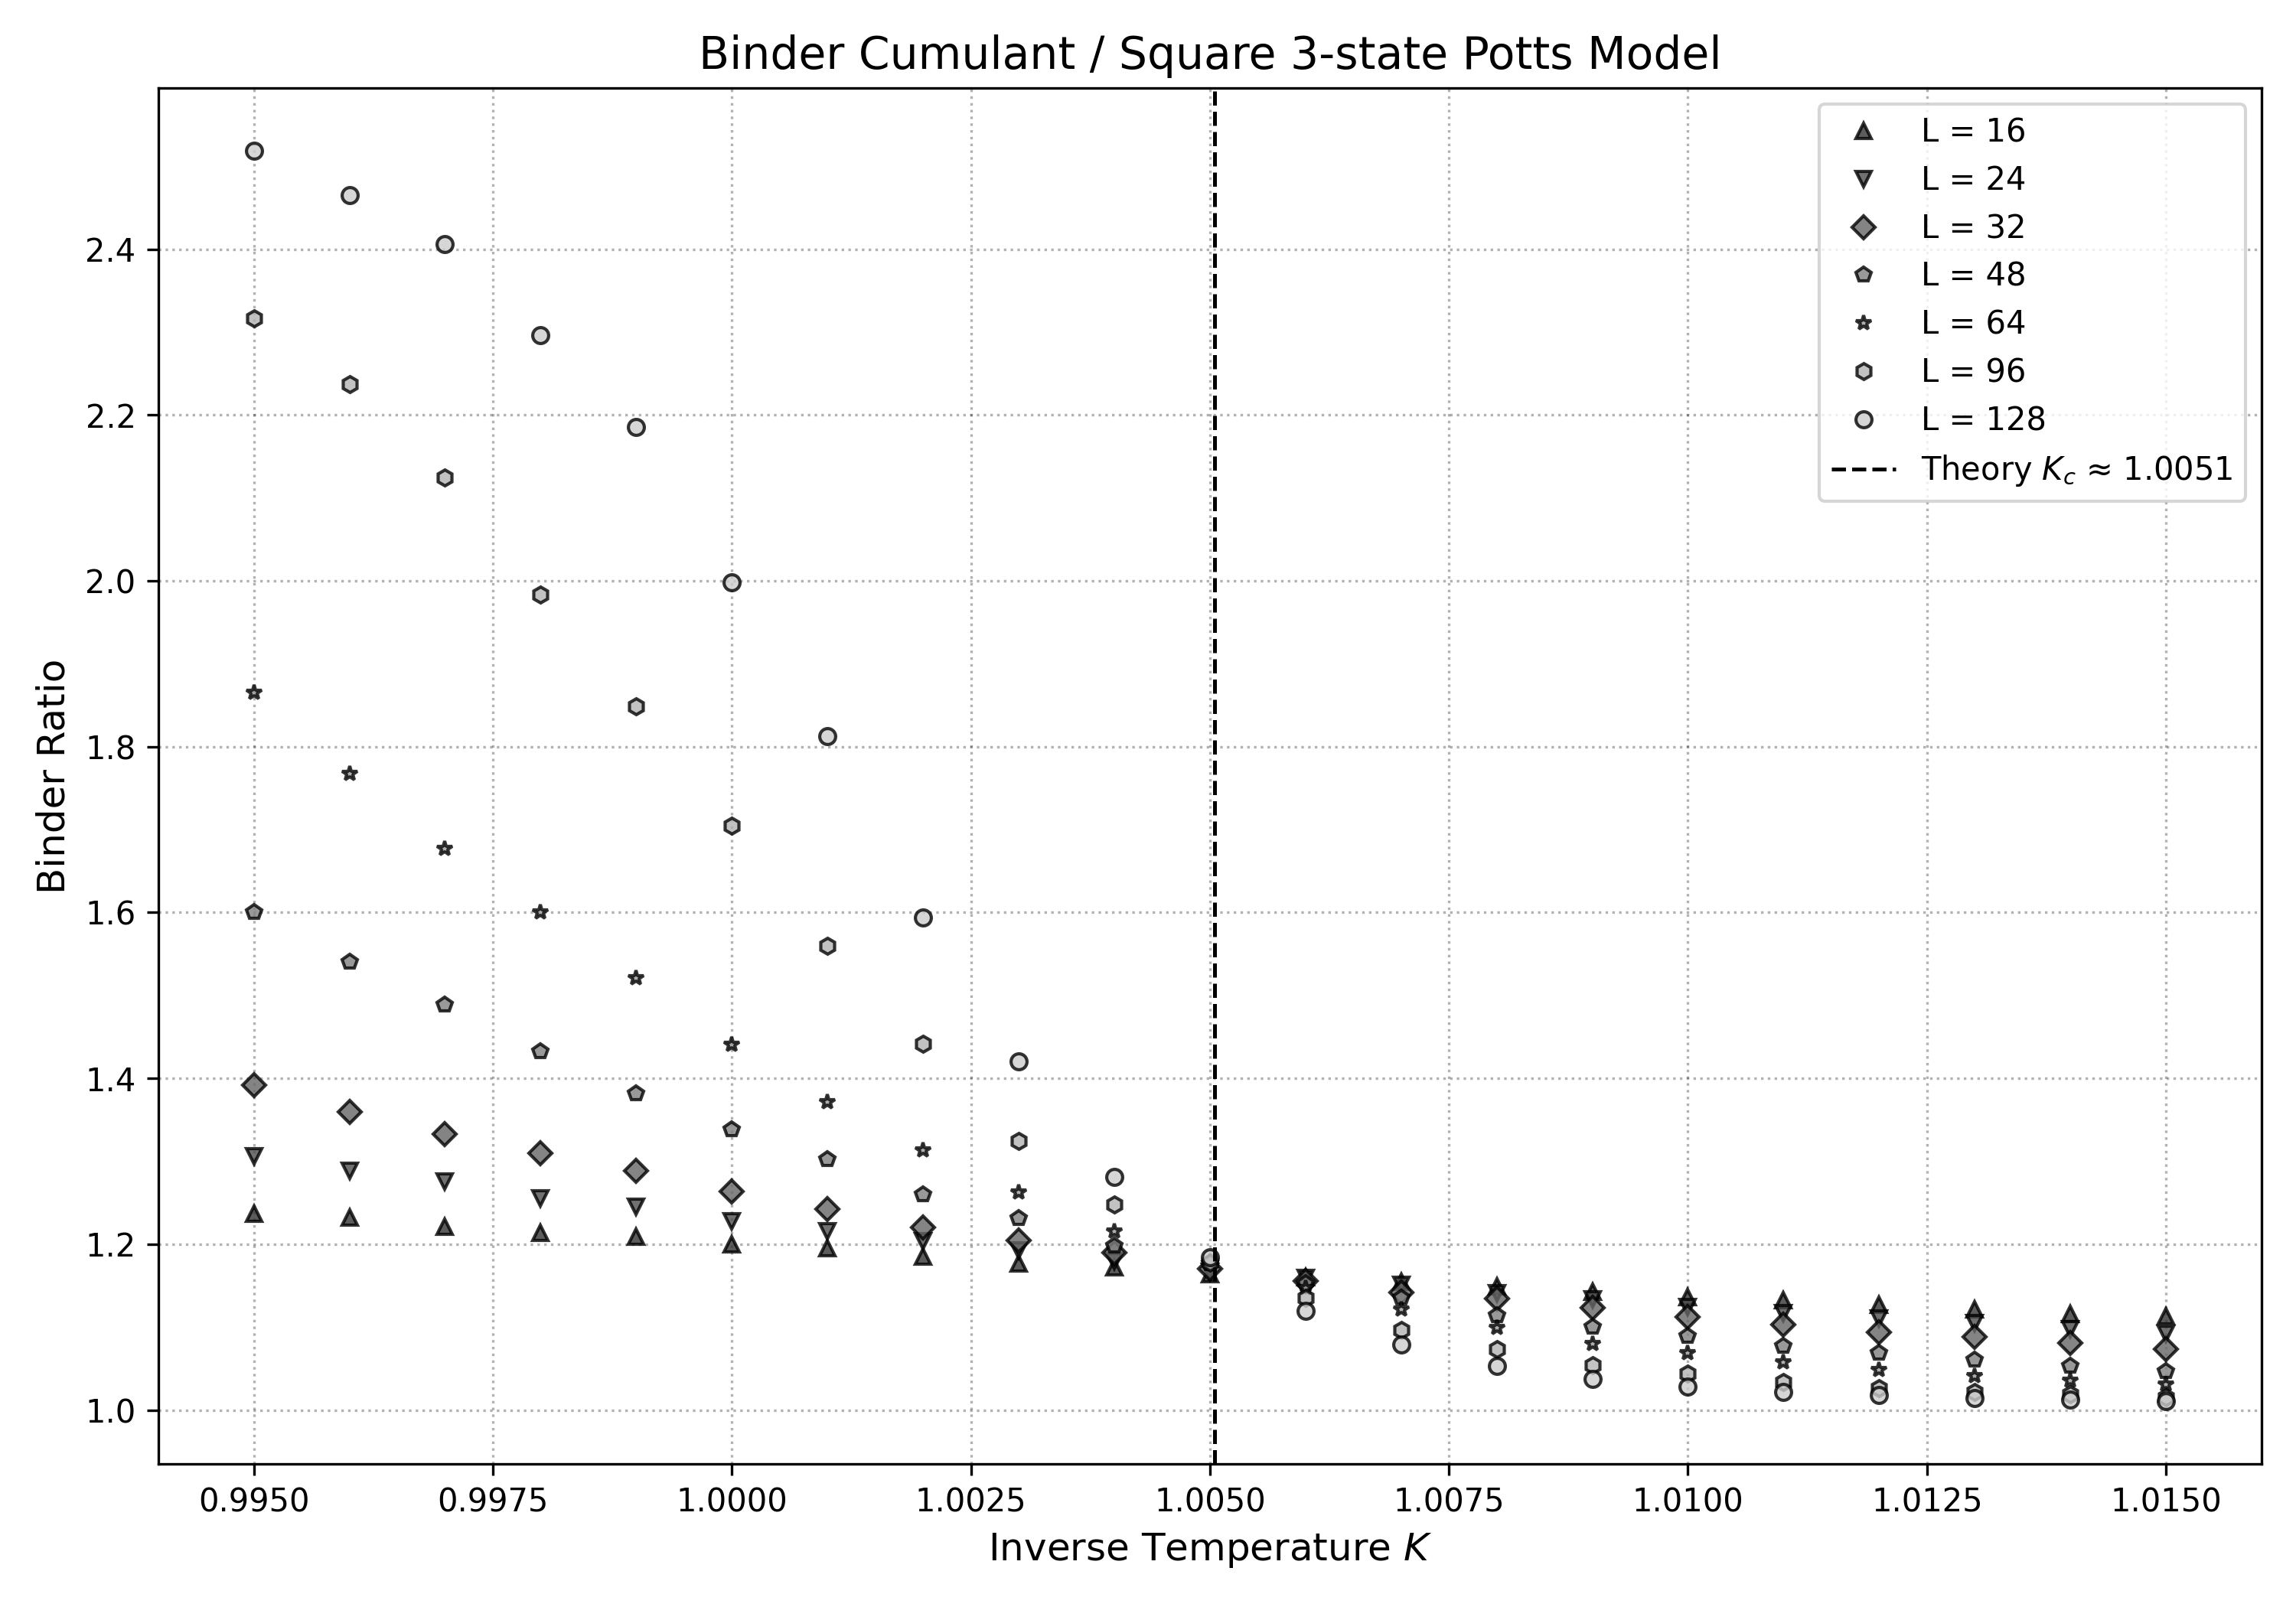
\includegraphics[width=\textwidth]{square_q3_potts_monochrome.png}
  \caption{正方格子上の3状態ポッツ模型のビンダー比}
  \label{fig:square_q3_potts}
\end{figure}
\begin{figure}[H]
  \centering
  % width=\textwidth でページ幅に合わせる
  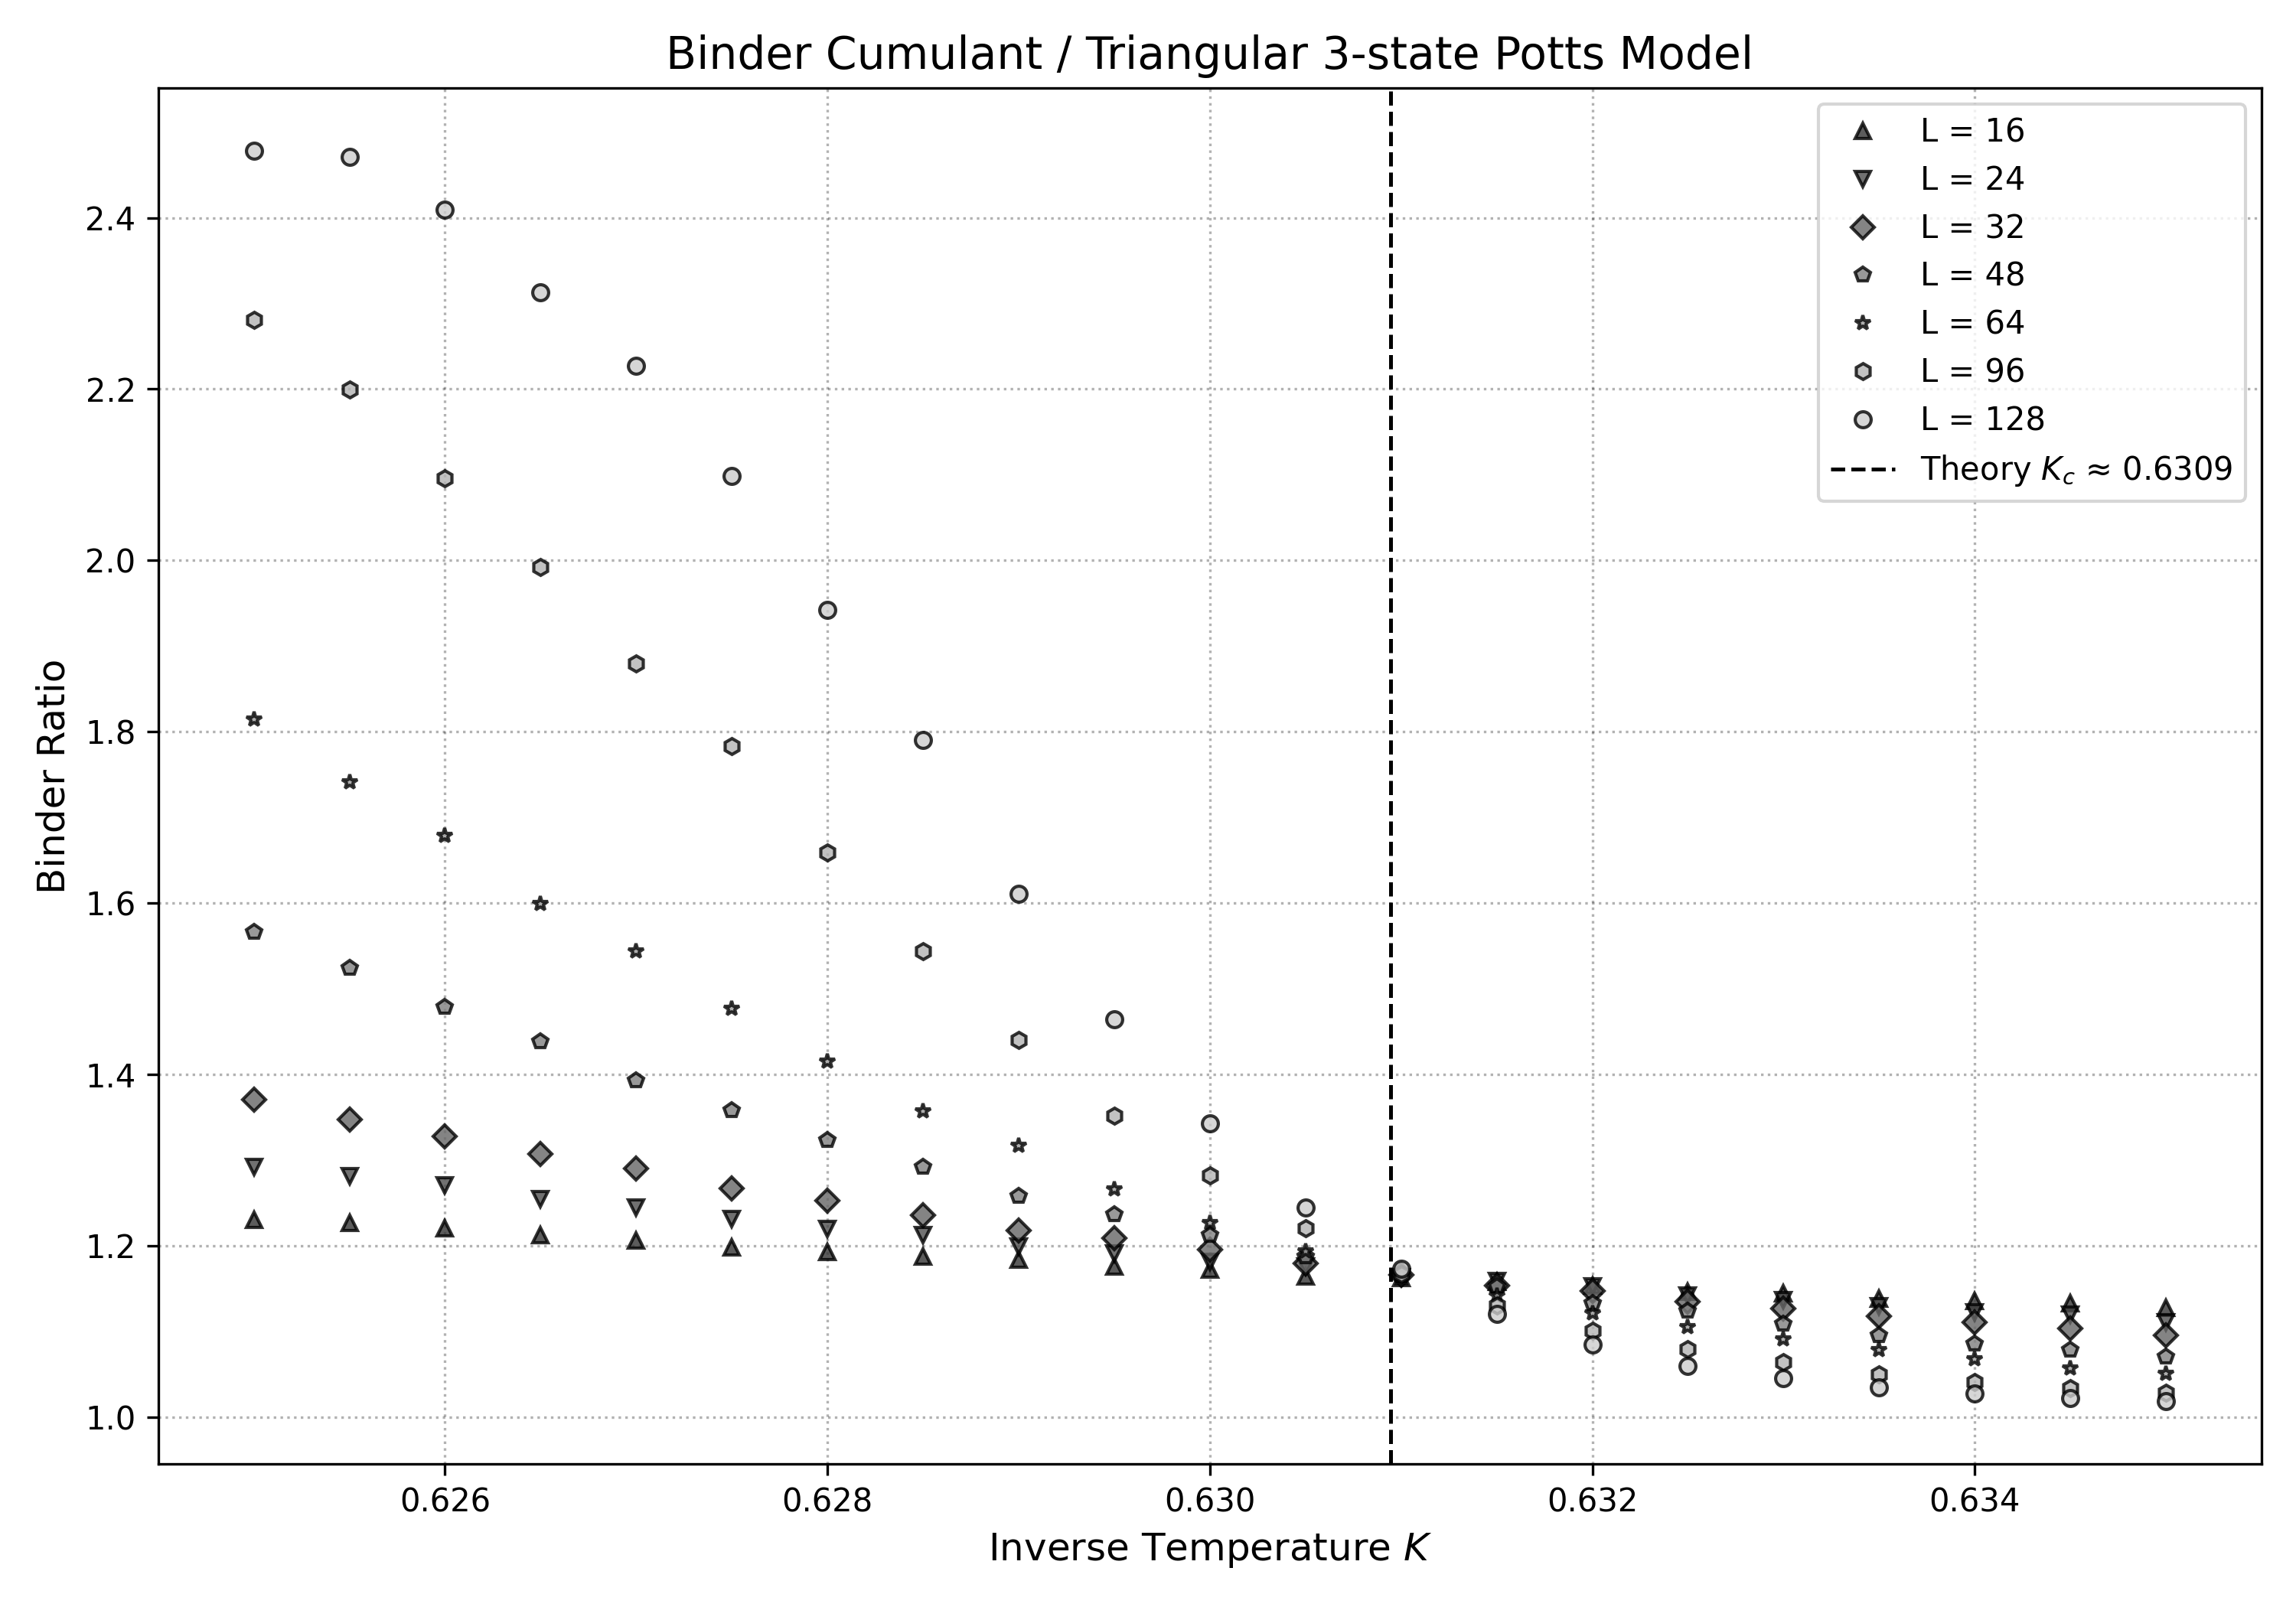
\includegraphics[width=\textwidth]{triangular_q3_potts_monochrome.png}
  \caption{三角格子上の3状態ポッツ模型のビンダー比}
  \label{fig:triangular_q3_potts}
\end{figure}
\begin{figure}[H]
  \centering
  % width=\textwidth でページ幅に合わせる
  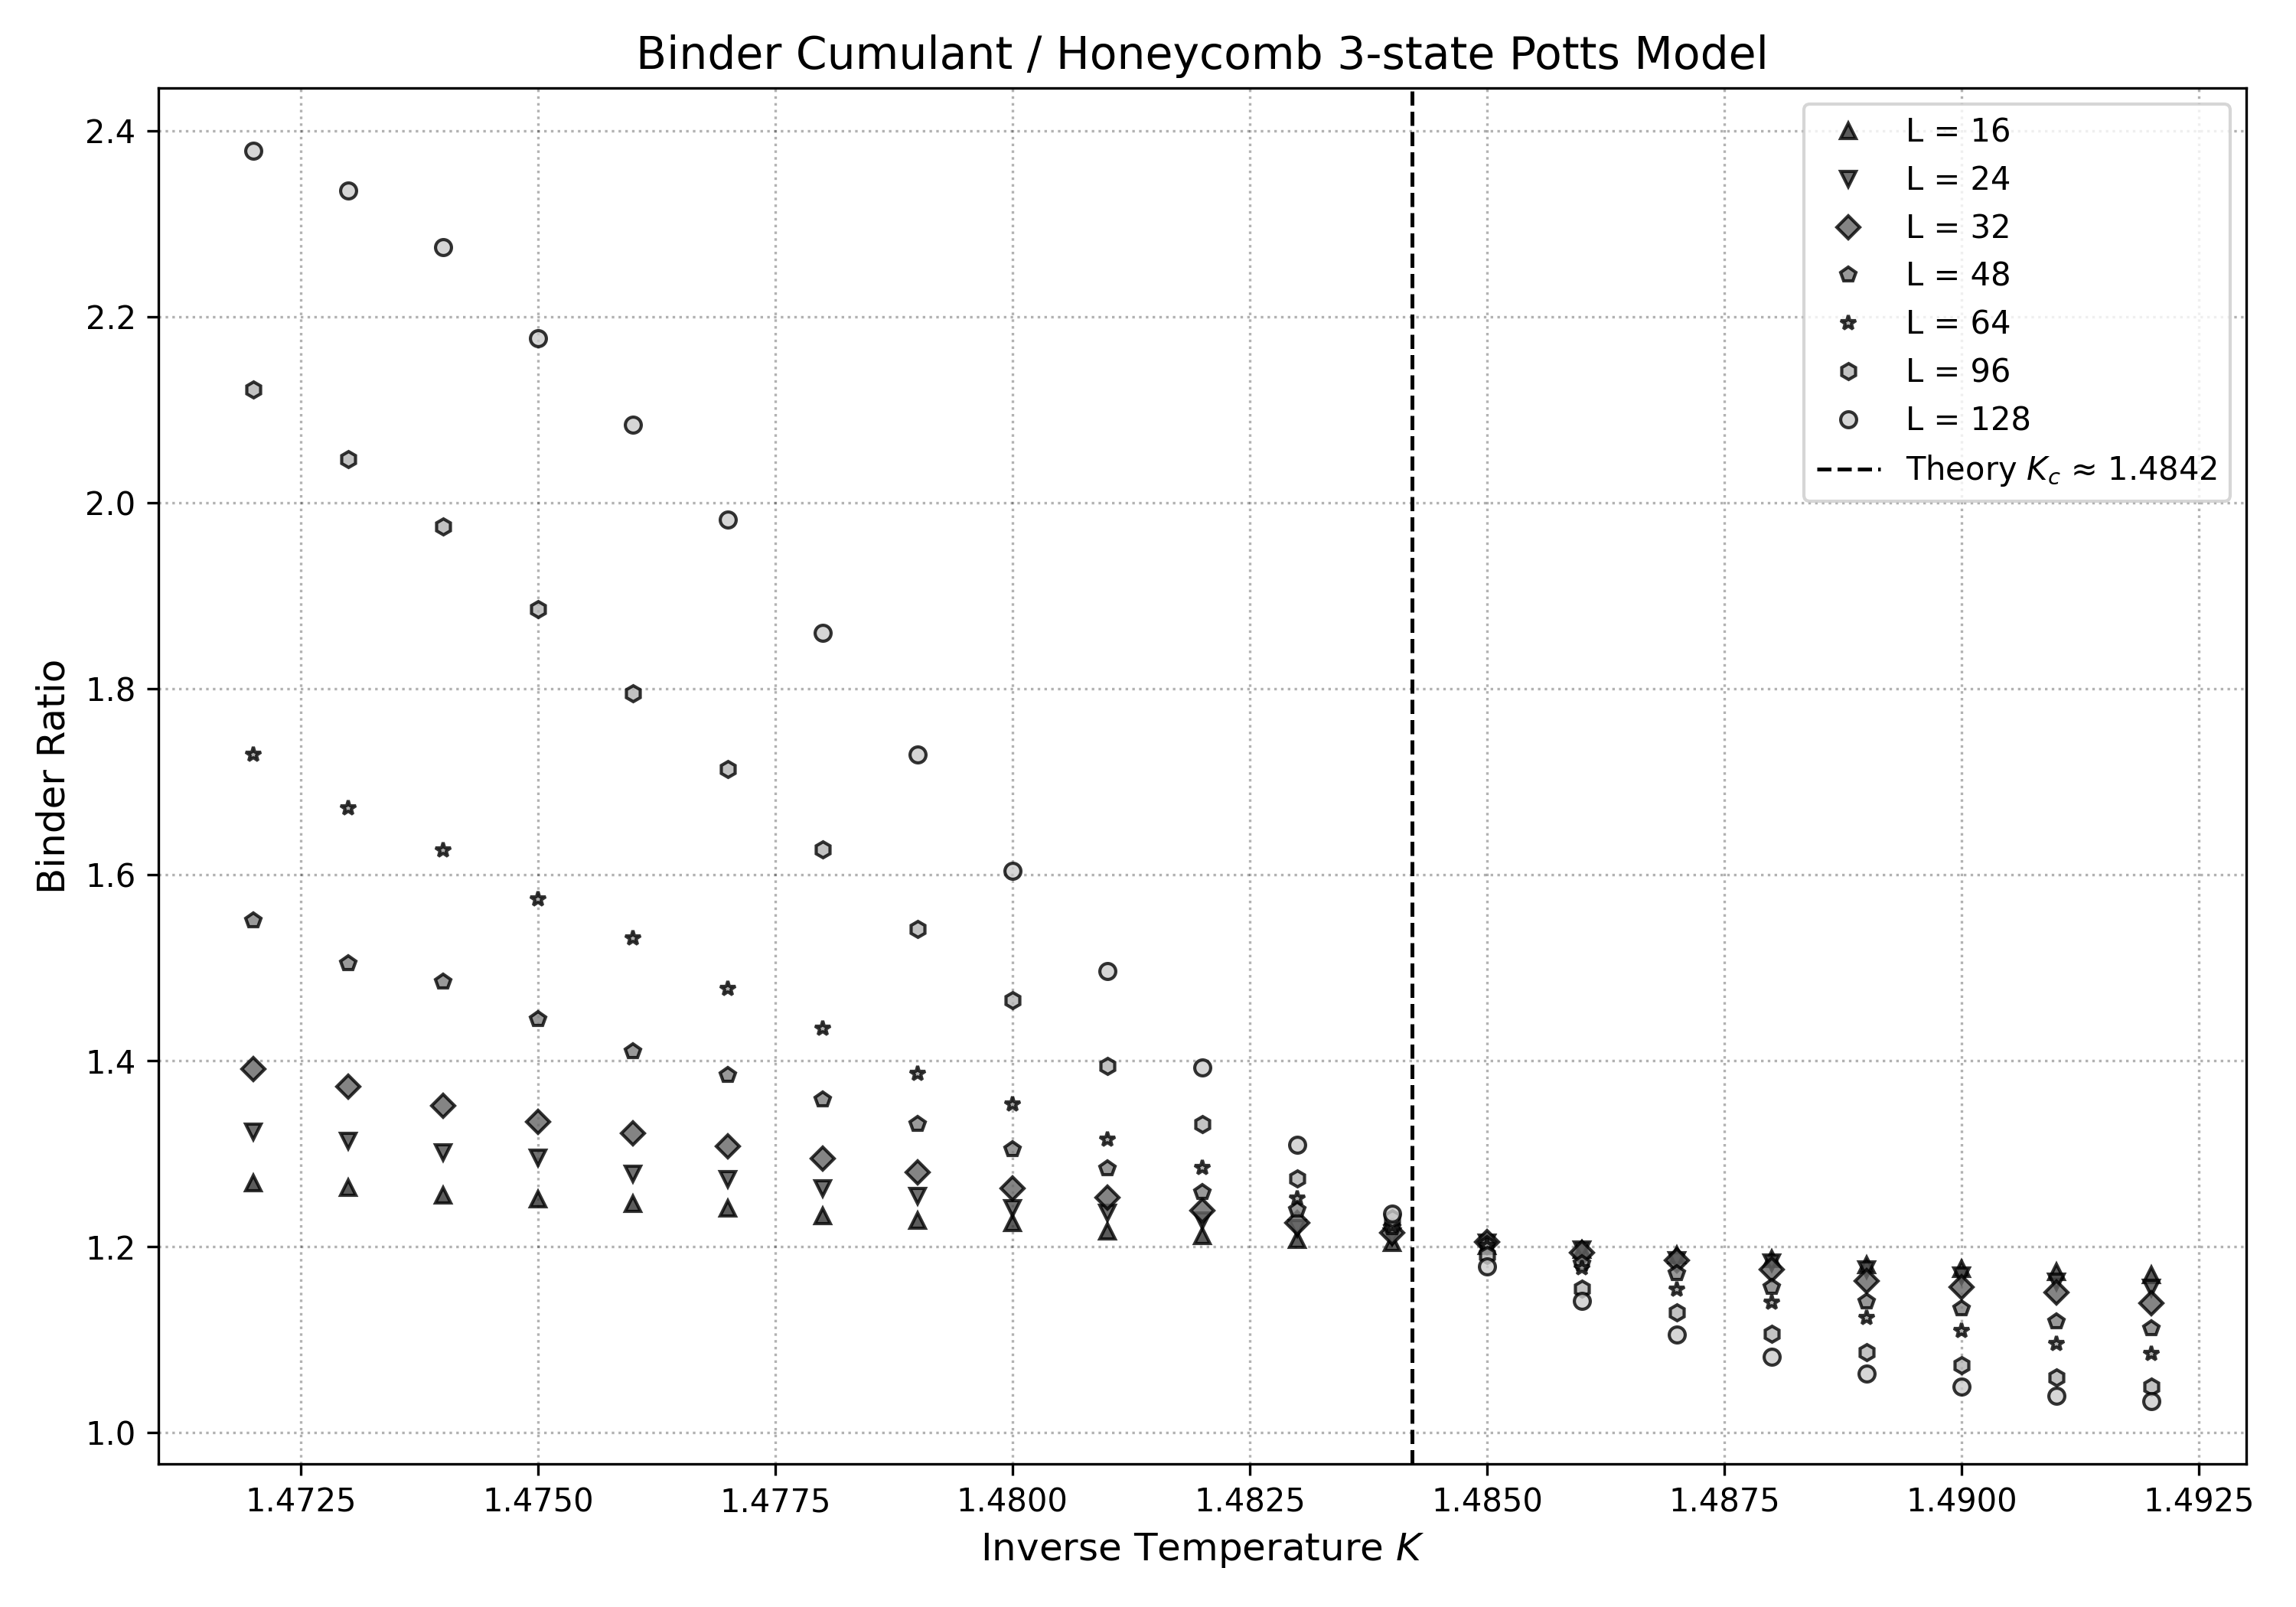
\includegraphics[width=\textwidth]{honeycomb_q3_potts_monochrome.png}
  \caption{蜂の巣格子上の3状態ポッツ模型のビンダー比}
  \label{fig:honeycomb_q3_potts}
\end{figure}

\begin{figure}[H]
  \centering
  % width=\textwidth でページ幅に合わせる
  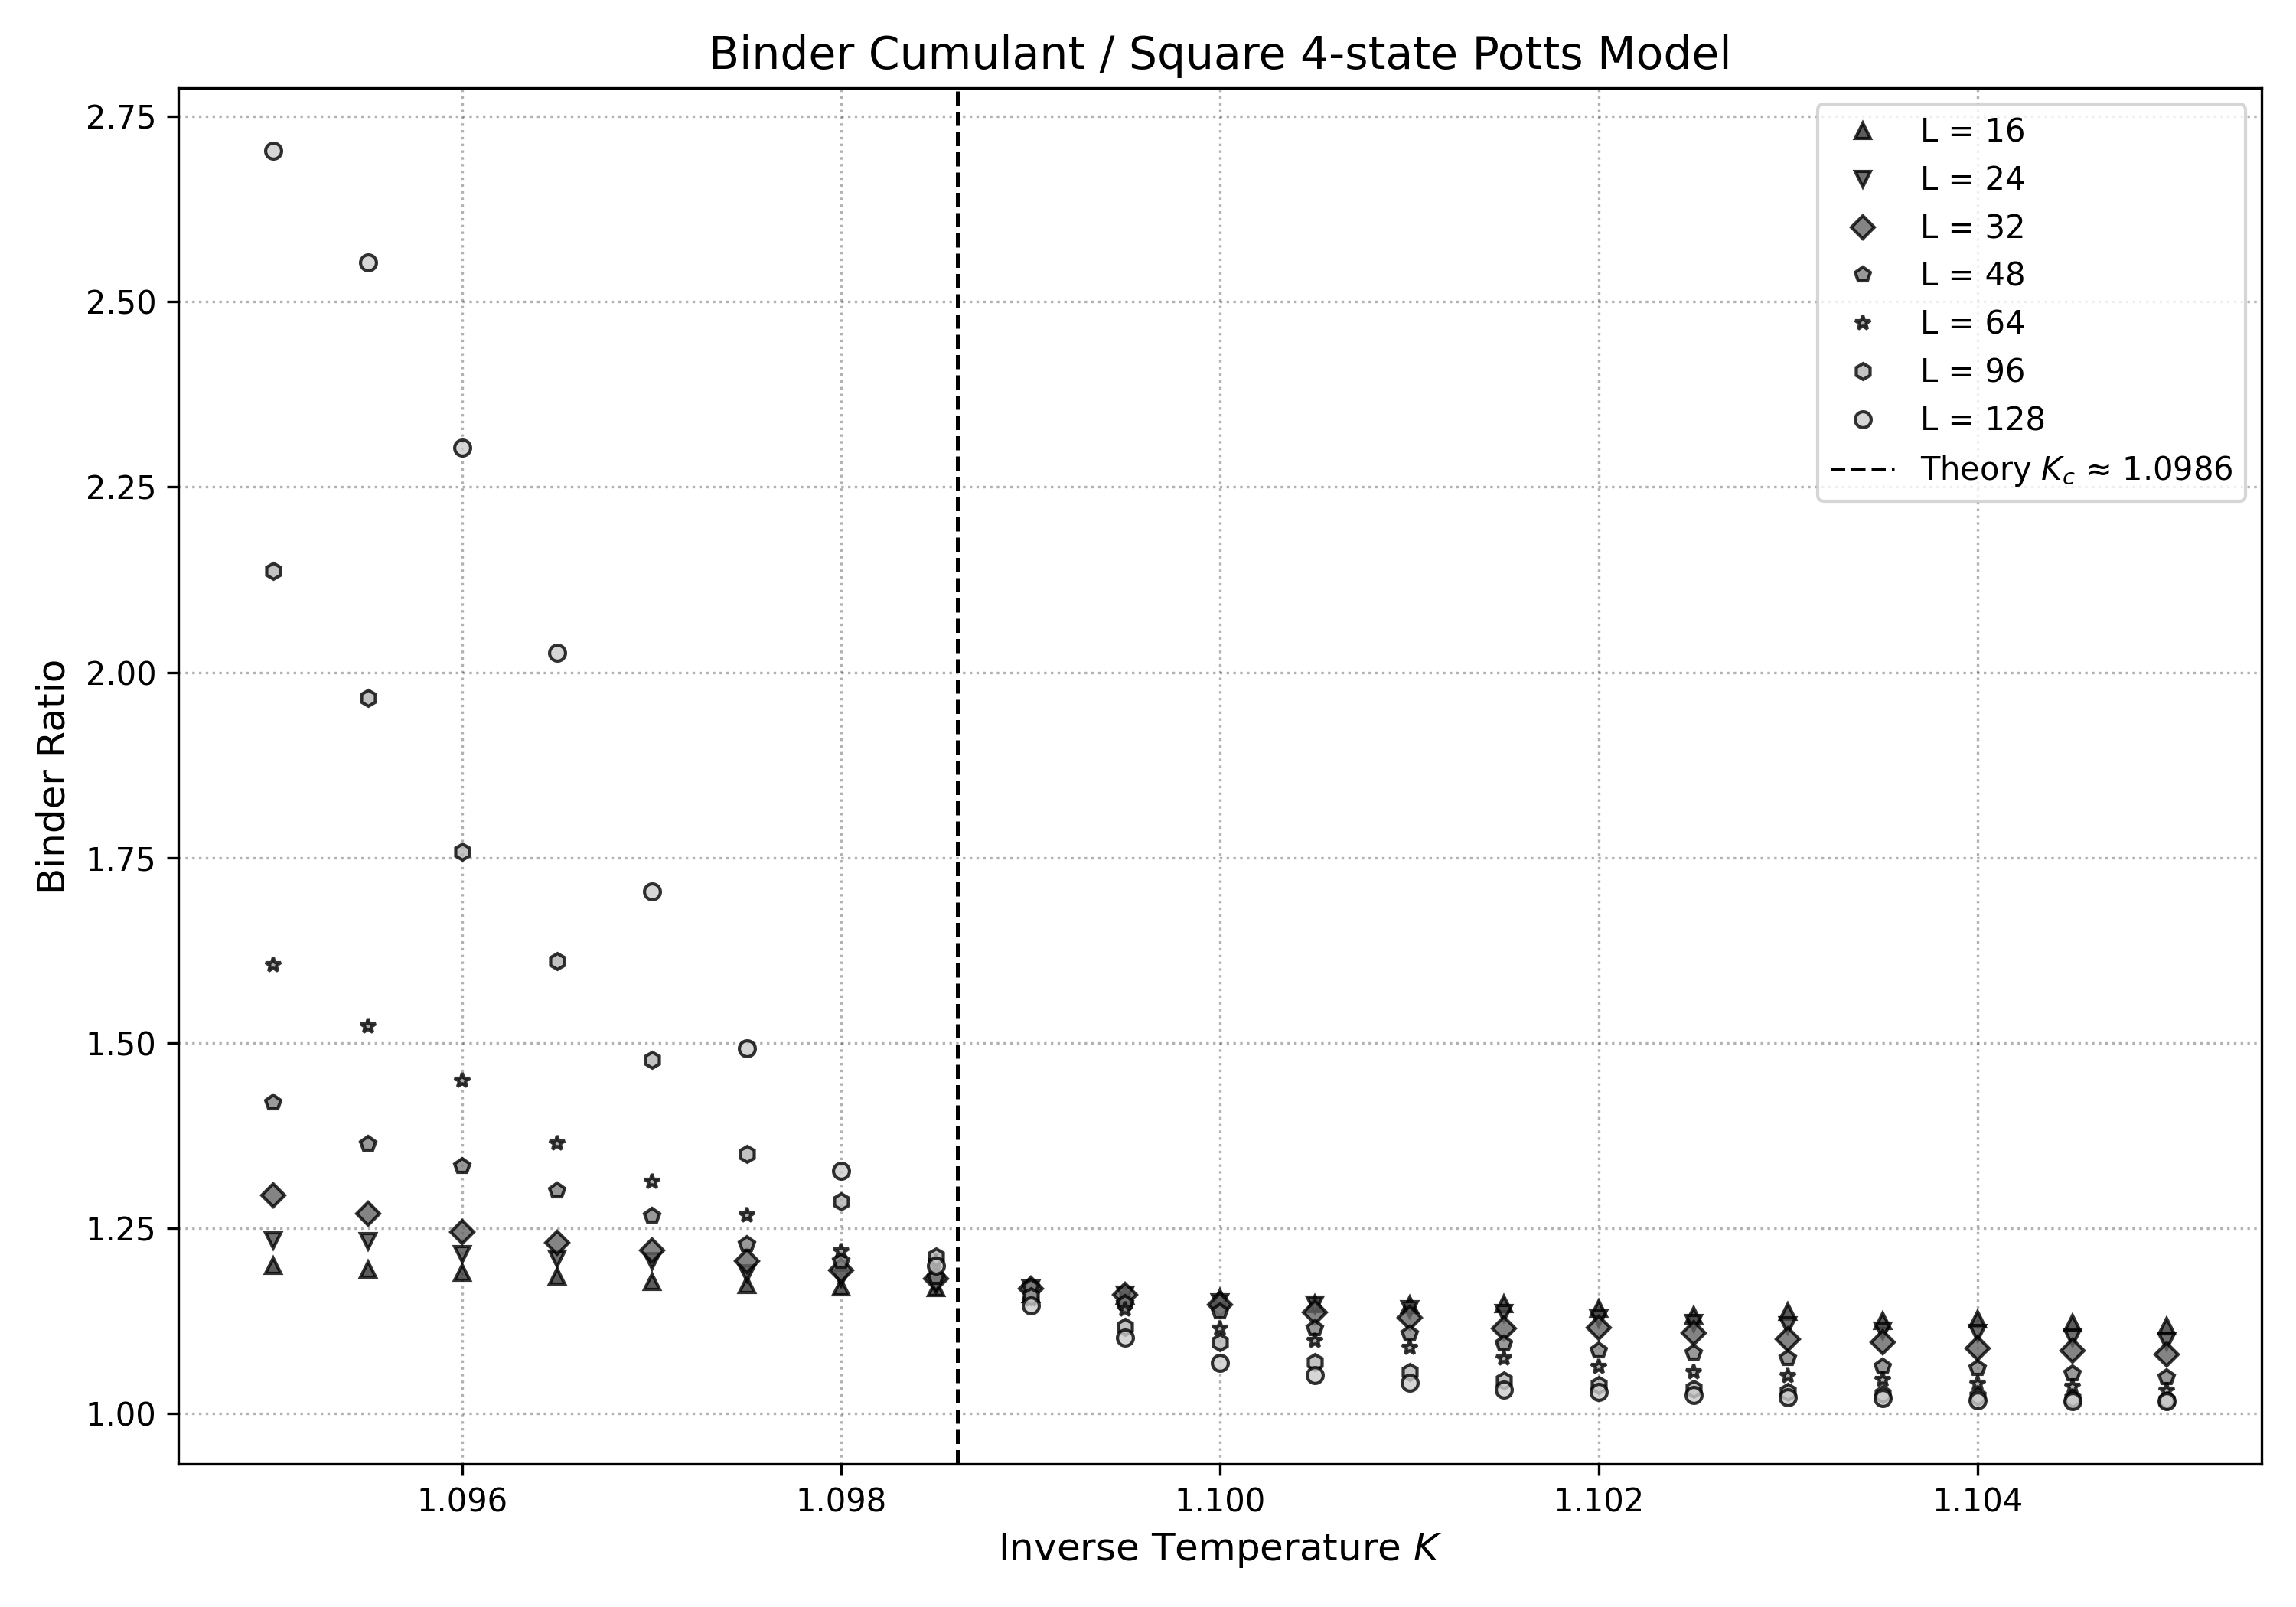
\includegraphics[width=\textwidth]{square_q4_potts_monochrome.png}
  \caption{正方格子上の4状態ポッツ模型のビンダー比}
  \label{fig:square_q4_potts}
\end{figure}
\begin{figure}[H]
  \centering
  % width=\textwidth でページ幅に合わせる
  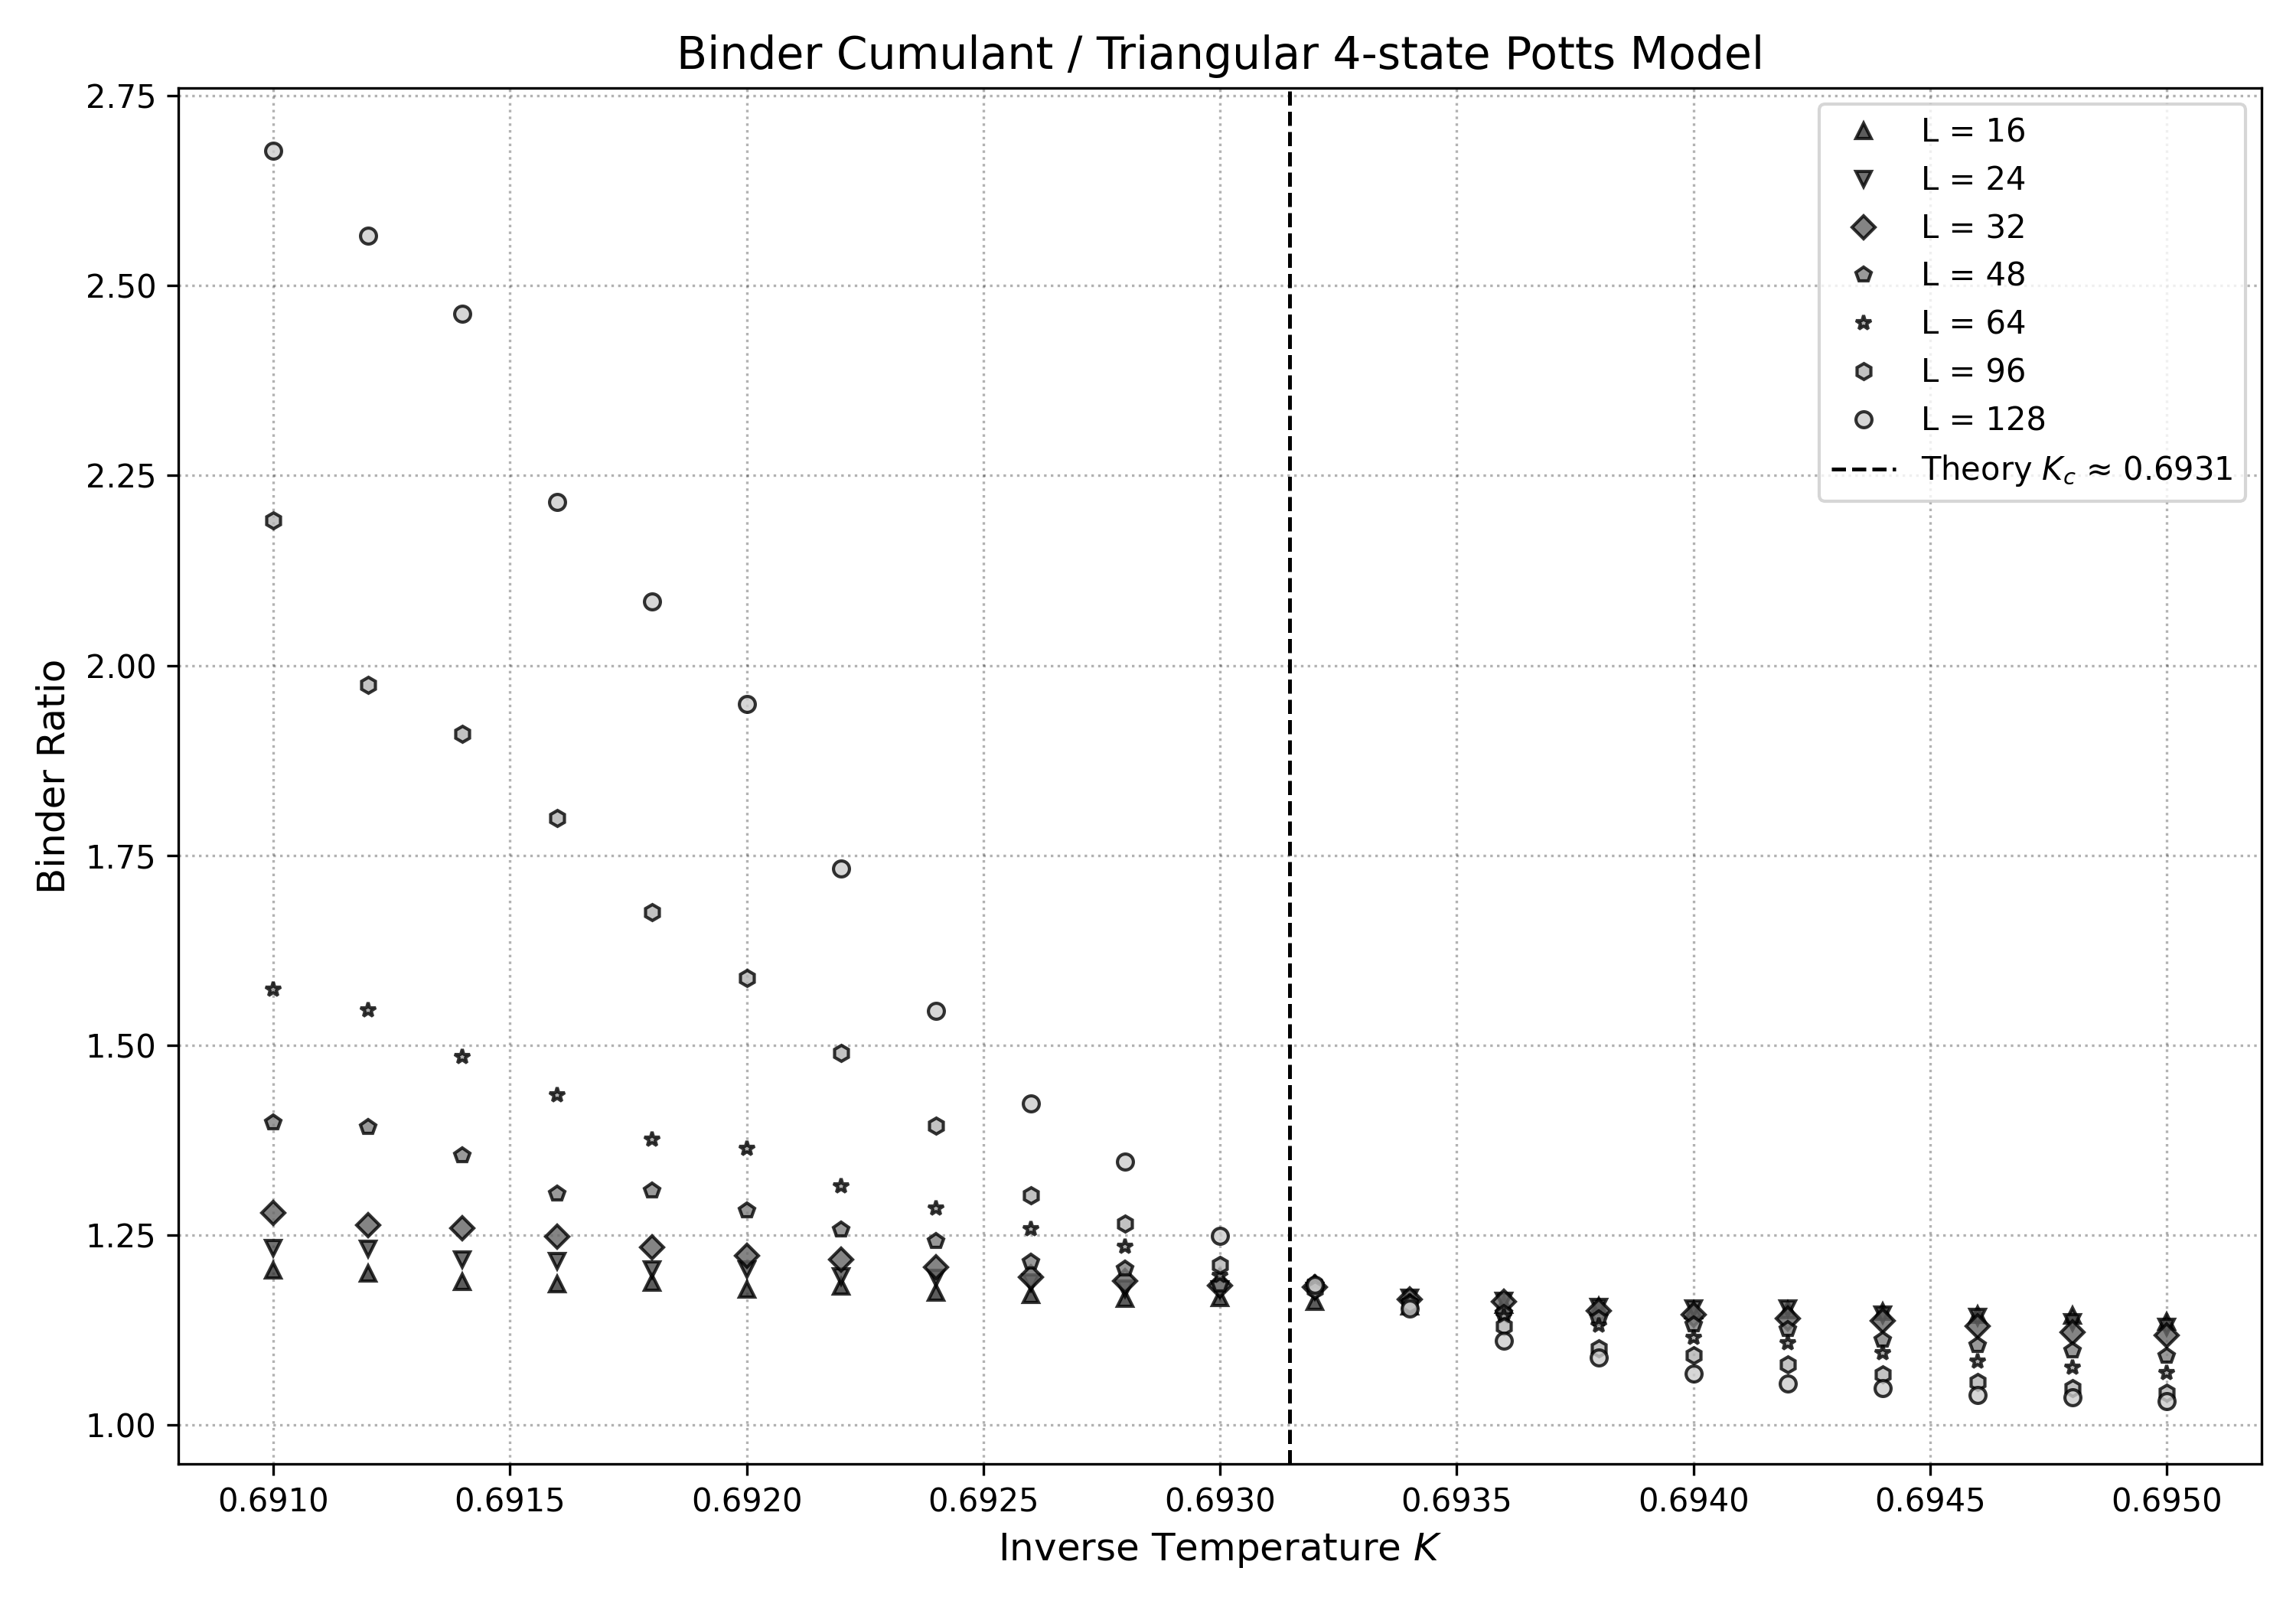
\includegraphics[width=\textwidth]{triangular_q4_potts_monochrome.png}
  \caption{三角格子上の4状態ポッツ模型のビンダー比}
  \label{fig:triangular_q4_potts}
\end{figure}
\begin{figure}[H]
  \centering
  % width=\textwidth でページ幅に合わせる
  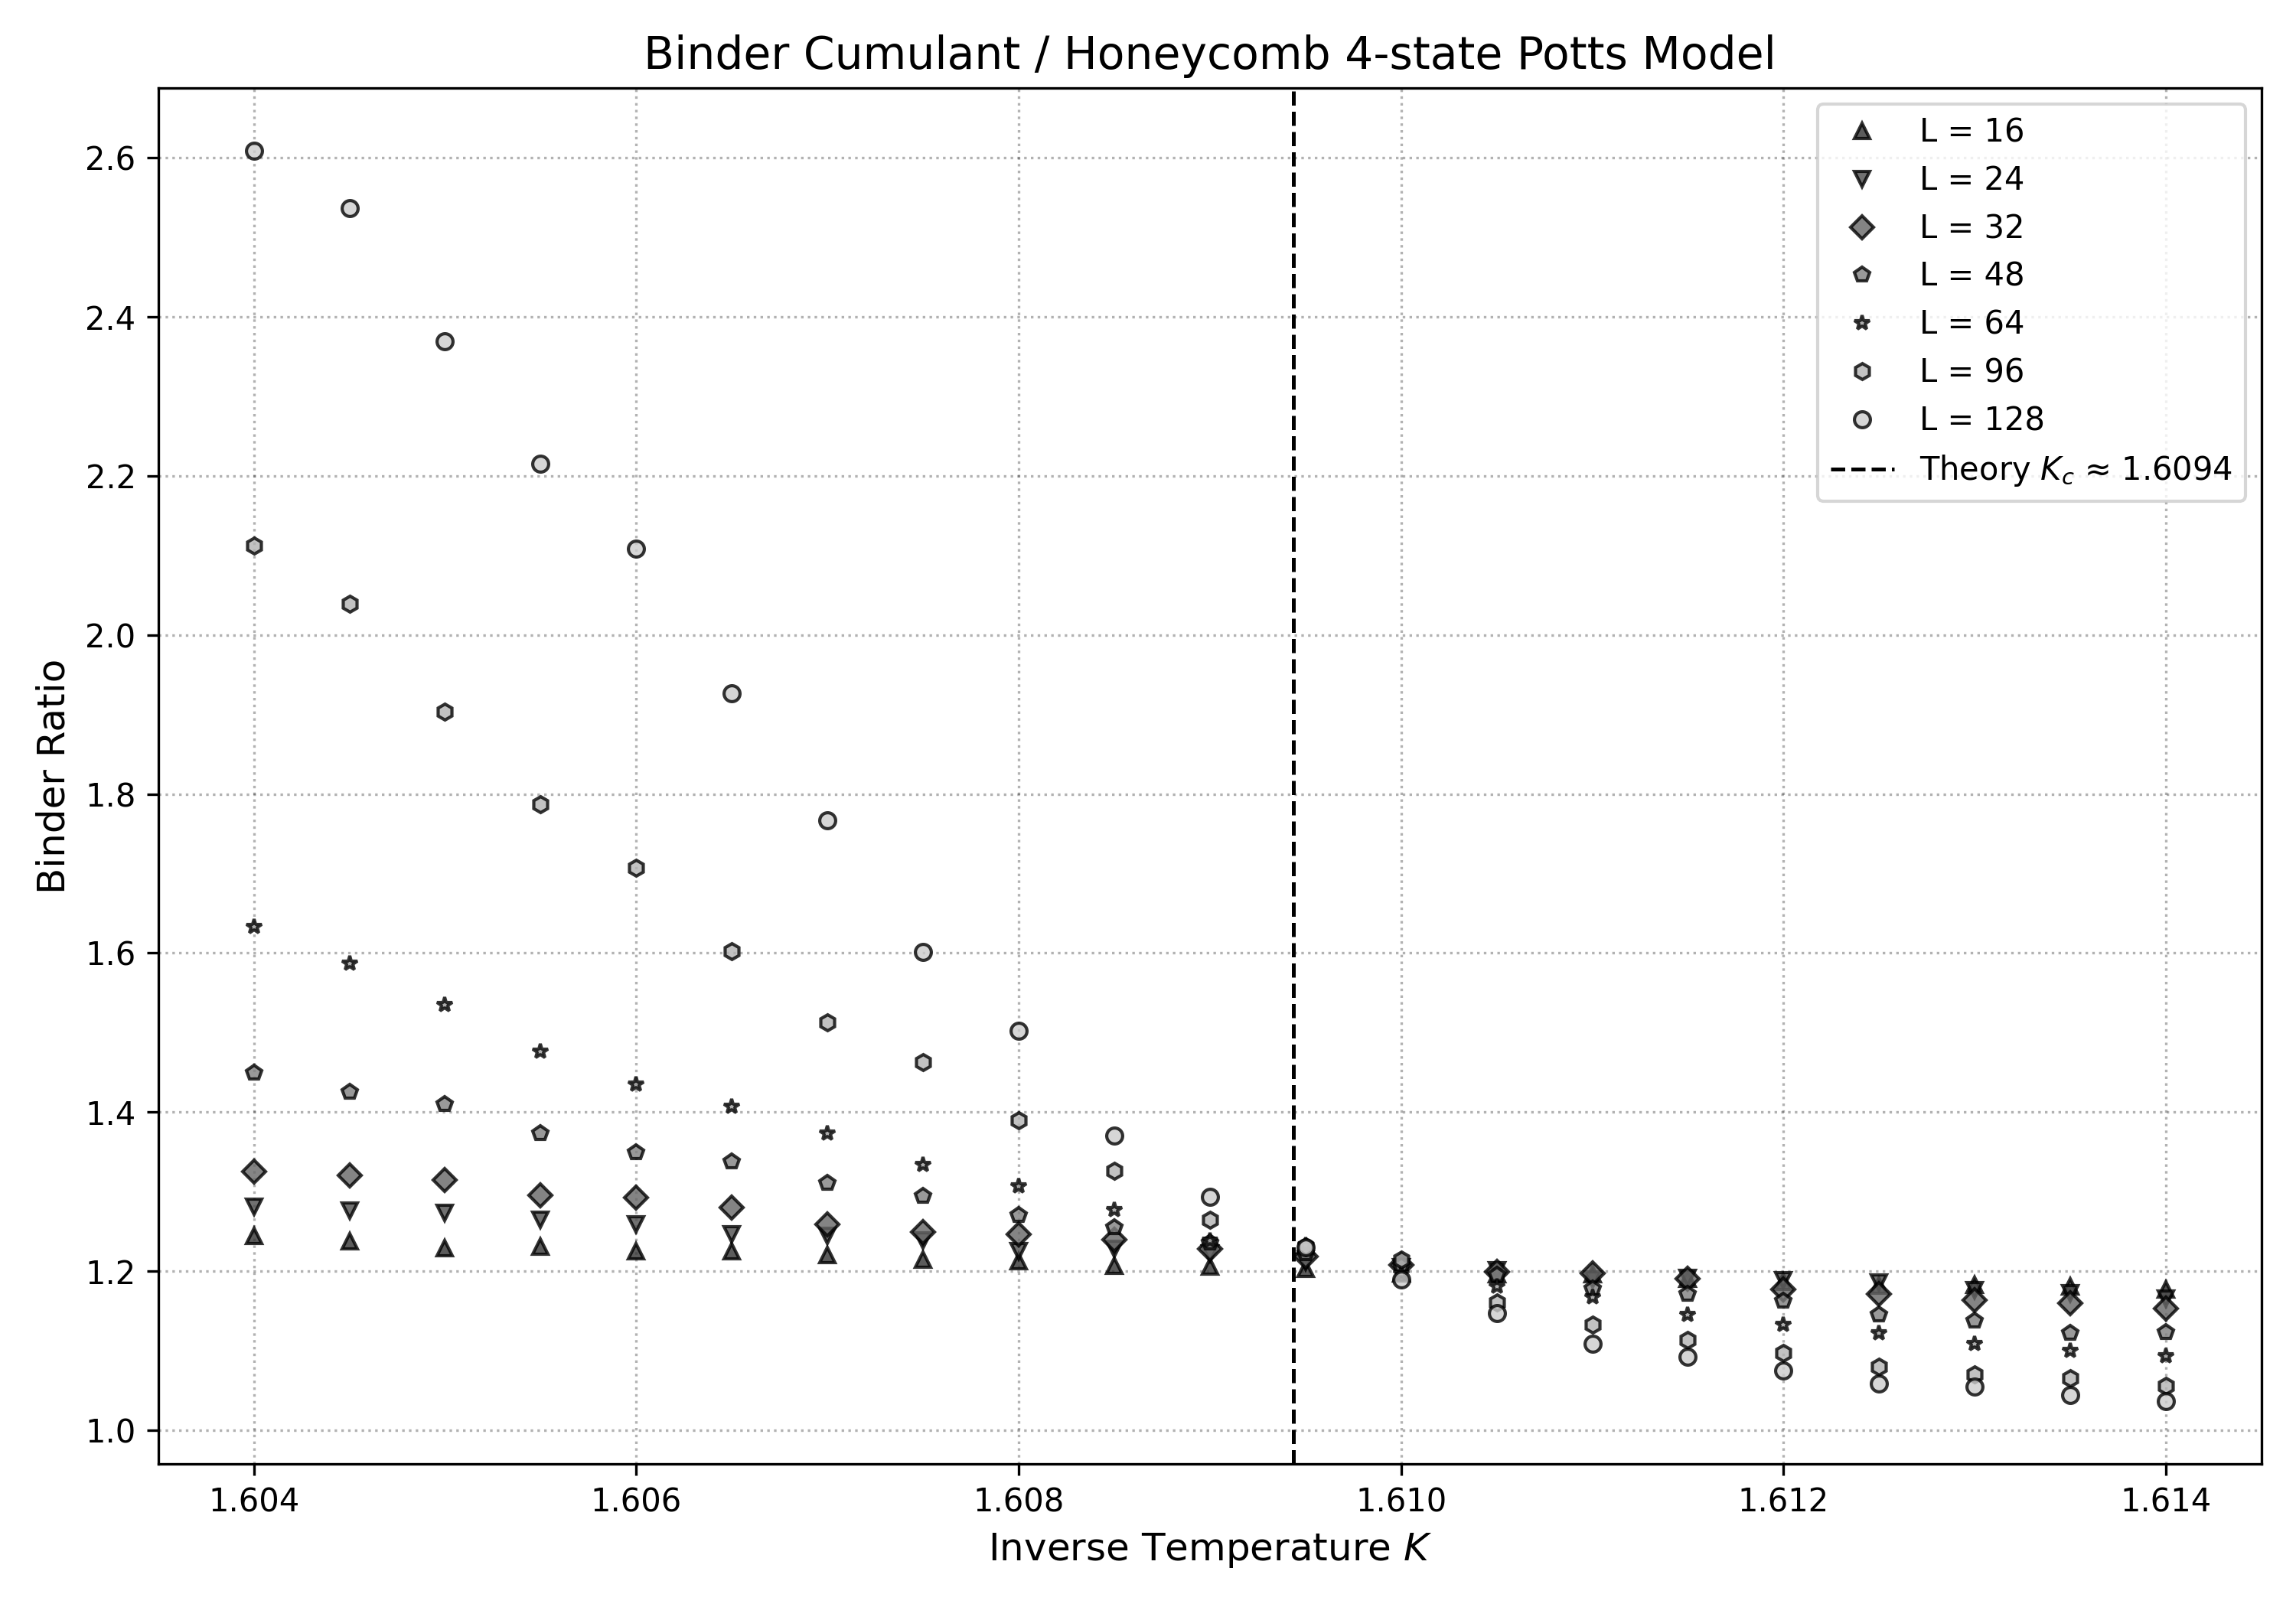
\includegraphics[width=\textwidth]{honeycomb_q4_potts_monochrome.png}
  \caption{蜂の巣格子上の4状態ポッツ模型のビンダー比}
  \label{fig:honeycomb_q4_potts}
\end{figure}

これでポッツ模型についても理解を深めることができた。つぎはちょっとだけ、反強磁性の場合の話を考えてみよう。

\subsubsection{反強磁性の場合}
\hiron ここまではずっと強磁性、つまり$J>0$の場合について考えてきたけど、ここでちょっとだけ、反強磁性、つまり$J<0$の場合になにが起こるか考えてみよう。まず、正方格子イジング模型の場合だけど、実は反強磁性$J<0$であっても、相互作用が$-J>0$であるような強磁性の模型と本質的に等価になる。どういうことかというと、こんなふうに1つおきにサイトを選んで副格子をつくる：

\begin{center}
\begin{tikzpicture}[scale=0.95]
  \foreach \x in {0,1,2,3,4} {
    \draw[gray!75, thick] (\x,0) -- (\x,4);
  }
  \foreach \y in {0,1,2,3,4} {
    \draw[gray!75, thick] (0,\y) -- (4,\y);
  }

  \foreach \x in {0,1,2,3,4} {
    \foreach \y in {0,1,2,3,4} {
      \pgfmathtruncatemacro{\parity}{mod(\x+\y,2)}
      \ifnum\parity=0
        \fill[black] (\x,\y) circle (2.6pt);
      \else
        \fill[white] (\x,\y) circle (2.6pt);
        \draw[black,thick] (\x,\y) circle (2.6pt);
      \fi
    }
  }
  \node[above, align=center, font=\small\bfseries] at (current bounding box.north) {
    2次元正方格子の副格子分解
  };
\end{tikzpicture}
\end{center}

そして、どちらかの副格子のすべてのスピンを一斉に反転すると、反強磁性の模型を強磁性の模型に、エネルギーの値やボルツマン重率を保ったままマッピングできる。いまの話では、正方格子を1つおきに2色で塗りわけられるという性質------つまり、格子が四角形という偶数角形だけでできている、二部グラフであるという性質------しか使っていないから、蜂の巣格子上のイジング模型についてもまったくおなじ議論が通用する：

\begin{center}
\begin{tikzpicture}[scale=0.95]
  % 単位ベクトルの成分（計算用）
  \pgfmathsetmacro{\dx}{1.73205} % sqrt(3)
  \pgfmathsetmacro{\dy}{1.5}

  \begin{scope}
    % 描画領域をクリップして端を綺麗に揃える
    \clip (-1.4, -0.9) rectangle (4.7, 3.7);

    % 蜂の巣格子の線
    \foreach \m in {-2,-1,0,1,2,3} {
      \foreach \n in {-2,-1,0,1,2,3} {
        \pgfmathsetmacro{\Ax}{\m*\dx + \n*\dx/2}
        \pgfmathsetmacro{\Ay}{\n*\dy}
        \pgfmathsetmacro{\Bx}{\Ax}
        \pgfmathsetmacro{\By}{\Ay + 1.0}
        \pgfmathsetmacro{\BdnLx}{\m*\dx + (\n-1)*\dx/2}
        \pgfmathsetmacro{\BdnLy}{(\n-1)*\dy + 1.0}
        \pgfmathsetmacro{\BdnRx}{(\m+1)*\dx + (\n-1)*\dx/2}
        \pgfmathsetmacro{\BdnRy}{(\n-1)*\dy + 1.0}

        \draw[gray!75, thick] (\Ax, \Ay) -- (\Bx, \By);
        \draw[gray!75, thick] (\Ax, \Ay) -- (\BdnLx, \BdnLy);
        \draw[gray!75, thick] (\Ax, \Ay) -- (\BdnRx, \BdnRy);
      }
    }

    % 頂点（A=黒, B=白）
    \foreach \m in {-2,-1,0,1,2,3} {
      \foreach \n in {-2,-1,0,1,2,3} {
        \pgfmathsetmacro{\Ax}{\m*\dx + \n*\dx/2}
        \pgfmathsetmacro{\Ay}{\n*\dy}
        \pgfmathsetmacro{\Bx}{\Ax}
        \pgfmathsetmacro{\By}{\Ay + 1.0}

        % 副格子A
        \fill[black] (\Ax, \Ay) circle (2.6pt);
        % 副格子B
        \fill[white] (\Bx, \By) circle (2.6pt);
        \draw[black, thick] (\Bx, \By) circle (2.6pt);
      }
    }
  \end{scope}
  \node[above, align=center, font=\small\bfseries] at (current bounding box.north) {
    蜂の巣格子の副格子分解
  };
\end{tikzpicture}
\end{center}

つまり、このふたつの模型ではそれぞれ強磁性の場合とおなじ温度で相転移が起こる。

つぎに三角格子上での反強磁性イジング模型がどうなるかを考える。千奈、三角格子の上の反強磁性イジング模型でエネルギー的にもっとも得をしている状態、つまり隣どうしのスピンがどこもちがう状態をつくるにはどうしたらいいかな？
\\\chinan ええと…………難しいですわ……。
\\\hiron ふふ……。
\\\chinan …………もしかして、どうやってもできないのではなくて？
\\\hiron ふふ、正解。
\\\chinan 篠澤さんがいじわるですわー！
\\\umen なんだか今日の広ちゃんはノリノリだね……。
\\\chinan そもそも三角形1つの時点で無理だと思いますわ！
\\\hiron ふふ……千奈の言うとおり、三角格子上の反強磁性イジング模型はすべてのボンドについてエネルギーを低い状態にすることができない。このことを、模型が\textbf{フラストレーションを持つ}という。もちろんこれは、三角格子が正方格子や蜂の巣格子のように二部グラフではないこと、それにともなってさっきみたいに副格子をとってスピンを反転させることで強磁性の場合に帰着できないことに対応している。じゃあこの模型の基底状態、つまりいちばんエネルギーが低い状態はどんなふうになっているかというと……たとえばこんなふうに構成できる。まず、三角格子を\textbf{3つの}副格子に分解する：

\begin{center}
\begin{tikzpicture}[scale=1.2]
  % 正三角形の高さ h = sqrt(3)/2
  \pgfmathsetmacro{\h}{sqrt(3)/2}

  % ==========================================
  % 格子と頂点の描画（はみ出さないようにクリップ）
  % ==========================================
  \begin{scope}
    \clip (-0.7, -0.5) rectangle (5.7, 3.8);

    % --- 線の描画 ---
    % 3方向の結合をループで一気に描画します
    \foreach \m in {-3,...,7} {
      \foreach \n in {-3,...,7} {
        \pgfmathsetmacro{\x}{\m + \n*0.5}
        \pgfmathsetmacro{\y}{\n*\h}
        
        \pgfmathsetmacro{\xOne}{\m+1 + \n*0.5}
        \pgfmathsetmacro{\yOne}{\n*\h}
        \pgfmathsetmacro{\xTwo}{\m + (\n+1)*0.5}
        \pgfmathsetmacro{\yTwo}{(\n+1)*\h}
        \pgfmathsetmacro{\xThree}{\m-1 + (\n+1)*0.5}
        \pgfmathsetmacro{\yThree}{(\n+1)*\h}

        \draw[gray!75, thick] (\x, \y) -- (\xOne, \yOne);
        \draw[gray!75, thick] (\x, \y) -- (\xTwo, \yTwo);
        \draw[gray!75, thick] (\x, \y) -- (\xThree, \yThree);
      }
    }

    % --- 頂点（3つの副格子）の描画 ---
    \foreach \m in {-3,...,7} {
      \foreach \n in {-3,...,7} {
        \pgfmathsetmacro{\x}{\m + \n*0.5}
        \pgfmathsetmacro{\y}{\n*\h}
        
        % 副格子の判定：(m - n) mod 3 と同等の計算
        % 負の数に対する剰余を避けるため十分大きな3の倍数を足しています
        \pgfmathsetmacro{\c}{int(mod(\m + 2*\n + 300, 3))}

        \ifnum\c=0
          % 副格子A: 赤い丸
          \fill[black] (\x, \y) circle (3pt);
        \fi
        \ifnum\c=1
          % 副格子B: 青い四角
          \fill[black] (\x-0.1, \y-0.1) rectangle (\x+0.1, \y+0.1);
        \fi
        \ifnum\c=2
          % 副格子C: 緑の三角
          \fill[black] (\x, \y+0.13) -- (\x-0.12, \y-0.08) -- (\x+0.12, \y-0.08) -- cycle;
        \fi
      }
    }
  \end{scope}

  % ==========================================
  % 凡例の描画
  % ==========================================
  \begin{scope}[xshift=6.2cm, yshift=1.6cm]
    % 凡例の枠
    \draw[gray!100, rounded corners] (-0.3, -1.2) rectangle (2.1, 0.9);
    
    % 副格子A（赤丸）
    \fill[black] (0, 0.3) circle (3pt);
    \node[font=\small, right] at (0.3, 0.3) {副格子 A};

    % 副格子B（青四角） 中心を(0, -0.2)に設定
    \fill[black] (-0.1, -0.3) rectangle (0.1, -0.1);
    \node[font=\small, right] at (0.3, -0.2) {副格子 B};

    % 副格子C（緑三角） 中心を(0, -0.7)に設定
    \fill[black] (0, -0.57) -- (-0.12, -0.78) -- (0.12, -0.78) -- cycle;
    \node[font=\small, right] at (0.3, -0.7) {副格子 C};
  \end{scope}

  \node[above, align=center, font=\small\bfseries] at (current bounding box.north) {
    三角格子の3副格子分解
  };
\end{tikzpicture}
\end{center}

\begin{comment}
\begin{center}
\begin{tikzpicture}[scale=1.2]
  % 正三角形の高さ h = sqrt(3)/2
  \pgfmathsetmacro{\h}{sqrt(3)/2}

  % ==========================================
  % 格子と頂点の描画（はみ出さないようにクリップ）
  % ==========================================
  \begin{scope}
    \clip (-0.7, -0.5) rectangle (5.7, 3.8);

    % --- 線の描画 ---
    % 3方向の結合をループで一気に描画します
    \foreach \m in {-3,...,7} {
      \foreach \n in {-3,...,7} {
        \pgfmathsetmacro{\x}{\m + \n*0.5}
        \pgfmathsetmacro{\y}{\n*\h}
        
        \pgfmathsetmacro{\xOne}{\m+1 + \n*0.5}
        \pgfmathsetmacro{\yOne}{\n*\h}
        \pgfmathsetmacro{\xTwo}{\m + (\n+1)*0.5}
        \pgfmathsetmacro{\yTwo}{(\n+1)*\h}
        \pgfmathsetmacro{\xThree}{\m-1 + (\n+1)*0.5}
        \pgfmathsetmacro{\yThree}{(\n+1)*\h}

        \draw[gray!45] (\x, \y) -- (\xOne, \yOne);
        \draw[gray!45] (\x, \y) -- (\xTwo, \yTwo);
        \draw[gray!45] (\x, \y) -- (\xThree, \yThree);
      }
    }

    % --- 頂点（3つの副格子）の描画 ---
    \foreach \m in {-3,...,7} {
      \foreach \n in {-3,...,7} {
        \pgfmathsetmacro{\x}{\m + \n*0.5}
        \pgfmathsetmacro{\y}{\n*\h}
        
        % 副格子の判定：(m - n) mod 3 と同等の計算
        % 負の数に対する剰余を避けるため十分大きな3の倍数を足しています
        \pgfmathsetmacro{\c}{int(mod(\m + 2*\n + 300, 3))}

        \ifnum\c=0
          % 副格子A: 赤い丸
          \fill[red!80] (\x, \y) circle (3pt);
        \fi
        \ifnum\c=1
          % 副格子B: 青い四角
          \fill[blue!80] (\x-0.1, \y-0.1) rectangle (\x+0.1, \y+0.1);
        \fi
        \ifnum\c=2
          % 副格子C: 緑の三角
          \fill[green!70!black] (\x, \y+0.13) -- (\x-0.12, \y-0.08) -- (\x+0.12, \y-0.08) -- cycle;
        \fi
      }
    }
  \end{scope}

  % ==========================================
  % 凡例の描画
  % ==========================================
  \begin{scope}[xshift=6.2cm, yshift=1.6cm]
    % 凡例の枠
    \draw[gray!50, rounded corners] (-0.3, -1.2) rectangle (2.1, 0.9);
    
    % 副格子A（赤丸）
    \fill[red!80] (0, 0.3) circle (3pt);
    \node[font=\small, right] at (0.3, 0.3) {副格子 A};

    % 副格子B（青四角） 中心を(0, -0.2)に設定
    \fill[blue!80] (-0.1, -0.3) rectangle (0.1, -0.1);
    \node[font=\small, right] at (0.3, -0.2) {副格子 B};

    % 副格子C（緑三角） 中心を(0, -0.7)に設定
    \fill[green!70!black] (0, -0.57) -- (-0.12, -0.78) -- (0.12, -0.78) -- cycle;
    \node[font=\small, right] at (0.3, -0.7) {副格子 C};
  \end{scope}

  \node[above, align=center, font=\small\bfseries] at (current bounding box.north) {
    三角格子の3副格子分解
  };
\end{tikzpicture}
\end{center}
\end{comment}

3つの副格子をA, B, C とする。副格子Aのスピンは$+1$, Bのスピンは$-1$にする。Cのスピンはそれぞれ好きなように決めていい。さっき確認したように、どの三角形についてもフラストレーションがあるから、これが基底状態の1つになる。このような状態がどのくらいあるかというと、系のスピンの数を$N$としたとき、だいたい$2^{N/3}$個くらいあることになる。実はこのパターン以外にも基底状態はあるから\footnote{興味があったらどんなパターンがあるか考えてみて、ね。}、基底状態の数はもうすこし多くなるけど、とにかく、この模型の基底状態には指数関数的に大きな数の縮退があることになる。強磁性のときの基底状態は全部$+$か全部$-$の2通りしかなかったから、これは決定的なちがい。そういう理由で、三角格子上の反強磁性イジング模型は有限温度で相転移しないことが知られている。ちなみに、この模型は基底状態の縮退数を厳密に求めることができて、サイト数$N$の系の基底状態の縮退数を$\Lambda_N$とすると、
\begin{align}
  W&\coloneqq\lim_{N\to\infty}(\Lambda_N)^{1/N},\\
  \log W &= \frac{2}{\pi} \int_0^{\pi/3} \log(2 \cos \omega) d\omega,\\
  W &\approx 1.38135,
\end{align}
になる。

つぎに反強磁性ポッツ模型について考える。$q=2$ではもちろんイジング模型とおなじだから、$q\ge3$とする。このとき、どの格子でもすべてのボンドのエネルギーを低い状態にとることができる。つまり、模型にフラストレーションはない。それどころか、正方格子や蜂の巣格子のときと、三角格子で$q\ge4$のときは、すべてのボンドのエネルギーが低い状態がやはり指数関数的にたくさん存在していて、基底状態に大きな数の縮退がある。だからこれらの場合は、フラストレーションは起こしていないけど、三角格子上のイジング模型とおなじように有限温度では相転移しないことになる。残りは三角格子で$q=3$の場合だけだけど、この場合だけ決定的にちがうことが起こる。佑芽、三角格子の上で隣り合うサイトどうしがどこもちがう色になるように、3色で塗りわけるにはどうしたらいいかな？
\\\umen またいじわるな問題じゃないよね……？
\\\hiron ふふ、大丈夫。こんどはちゃんと、おもしろい答えになる。千奈もやってみて。
\\\chinan わかりましたわ！
\\
------再び数分後。
\\\chinan …………できたと思いますわ！
\\\umen あたしもできた気がする！
\\\hiron ……たしかにふたりともできてる、ね。やってみて、なにか気づいたことはなかった？
\\\chinan …………もしかして、一部を決めると全体が決まってしまうのではなくて……？
\\\umen それはあたしも思ったかも！　それにしても、この塗りかた、どこかで見たような……？
\\\hiron ふふ……。
\\\umen …………あ！　わかった！　さっきの副格子分解の図とおなじだ！
\\\hiron ふふ、正解。三角格子で$q=3$のとき、すべてのボンドのエネルギーが低い状態になるようにする方法は、本質的にひとつの方法しかない。3つある副格子のそれぞれで、すべてのスピンがおなじ状態になって、ちがう副格子はちがう状態になるようにする……それしか方法はない。じゃあそうする方法は、ちゃんと数えたら全部で何通りくらいあると思う？
\\\chinan ええと…………。
\\\umen うーん…………。
\\\hiron ……ちなみにふたりとも、実はこの問題は解けないとまずい。
\\\umen ええ！？
\\\hiron 統計力学の話じたいは結構むずかしいことをやってるし、学校の試験には出ないから、最悪理解できなくても大丈夫。でも、この問題は簡単な組み合わせの問題だから、ふたりとも解けないと補習になっちゃうかも\footnote{まあ、わたしは座学を免除されているから、授業の詳しい進度はよくわからないけど。}。
\\\umen むむむ…………。
\\\chinan …………わかりましたわ！　もともと3つある副格子にどの色を順番に当てはめるかという問題ですから、答えは$3!=6$通りでしょうか？
\\\hiron 千奈、正解。佑芽は復習しておくように。
\\\umen ぐぬぬ……。
\\\hiron 話をもとに戻そう。三角格子上の反強磁性$q=3$ポッツ模型は、系の大きさにかかわらず基底状態が6通りしかない。これは正方格子イジング模型のときと同様に、じゅうぶん少ない縮退数。この性質により、この模型は有限温度で相転移が起こる。ちなみに相転移の次数は、2次元系ではめずらしい``弱い1次相転移''というクラスに属する。この模型の転移温度はいままでの計算とおなじような方法を使うことができず、残念ながら厳密な値は知られていない。話がすこし複雑になったから、反強磁性の場合について、各格子と$q$の値ごとに相転移の様子を表にまとめておこう：

\begin{center}
\begin{tabular}{c||c|c|c|c}
  \hline
  格子 & $q=2$ & $q=3$ & $q=4$ & $q\ge5$ \\
  \hline\hline
  蜂の巣格子 & 2次相転移 & なし（※2） & なし（※2） & なし（※2）\\
  \hline
  正方格子 & 2次相転移 & なし（※1） & なし（※2） & なし（※2）\\
  \hline
  三角格子 & なし（※1） & 弱い1次相転移 & なし（※1） & なし（※2）\\
  \hline
\end{tabular}

\begin{tabular}{@{}ll@{}}
※1 & 絶対零度で相関関数が冪乗減衰する（臨界相）\\
※2 & 絶対零度で相関関数が指数関数的に減衰する（無秩序相）
\end{tabular}
\end{center}

表に書いたように、有限温度で相転移しない模型のうち、状態数$q$が少ないものや格子の配位数が多いものは基底状態の数が少ないから、絶対零度での相関関数の減衰のしかたに違いが見られる、よ。反対に$q$を増やしていくとそのような秩序はなくなっていく傾向がある。でもこの話題はむずかしい話になるから深入りは避けておこう。

ちなみに反強磁性ポッツ模型は正方格子で $q=3$のときと三角格子で $q=4$ のときに基底状態の縮退数を厳密に求めることができて、1サイトあたりの縮退数は正方格子で $q=3$のとき
\begin{align}
  W = \left( \frac{4}{3} \right)^{3/2} \approx 1.5396,\label{eq:n_degeneracy_afm_q=3_square}
\end{align}
三角格子で $q=4$ のとき
\begin{align}
  W_{\mathrm{tri}} = \frac{\Gamma(1/3)}{\Gamma(2/3)^2} \approx 1.4609,
\end{align}
になる。ちなみにこの縮退数$W_{\mathrm{tri}}$は、蜂の巣格子のエッジを3彩色するときの1サイトあたりの場合の数$w$と$W_{\mathrm{tri}}=w^2$という対応がある。これはおもしろい方法で示せるからやってみよう。

まず、三角格子を彩色する4つの色を$(a,b)\in(\mathbb F_2)^2$で表す。つぎに、三角格子と蜂の巣格子は互いに双対な格子だから、これらを辺が直交するように重ねて描く。このとき蜂の巣格子の辺と三角格子の辺が1対1に対応するけど、三角格子のサイト$i$, $j$の色を$\sigma_i$, $\sigma_j$としたとき、それらをつなぐ辺に対応する蜂の巣格子の辺の色$E_{ij}$を、
\begin{align}
  E_{ij} = \sigma_i + \sigma_j,
\end{align}
と定める。いま、三角格子は4彩色されていて、$\sigma_i\ne\sigma_j$だから、$E_{ij}$は決して$(0,0)$にならない。つまり、この方法で蜂の巣格子の辺を3色で塗る方法が得られることになる。この塗り方が3彩色のルール、つまり共有点を持つ辺がおなじ色にならないこともチェックしよう。蜂の巣格子のある頂点に集まる3本の辺$E_1$, $E_2$, $E_3$は、三角格子の1つの三角形の3つの辺$ij$, $jk$, $ki$に対応しているから、
\begin{align}
  E_1 &= \sigma_i + \sigma_j,\\
  E_2 &= \sigma_j + \sigma_k,\\
  E_3 &= \sigma_k + \sigma_i,
\end{align}
になる。これらを足し合わせると、
\begin{align}
  E_1+E_2+E_3=0.
\end{align}
これは$E_1$, $E_2$, $E_3$がすべて異なるときにしか起こらない。これで三角格子の4彩色から蜂の巣格子の3彩色を得る方法がわかった。この対応は$(\mathbb F_2)^2$への色の対応のさせ方が4彩色と3彩色でそれぞれ$4!$通り、$3!$通りある。だから状態の総数、つまり分配関数$Z$について、
\begin{align}
  \frac1{4!}Z_{\mathrm{tri},q=4}=\frac1{3!}Z_{\mathrm{hex, edge, 3-colour}},\label{eq:relation_n_states_triangular_honeycomb}
\end{align}
がなりたつ。サイト数$N$の三角格子を双対蜂の巣格子に変換するとサイト数が$2N$になることと、(\ref{eq:relation_n_states_triangular_honeycomb})において$N$が大きいときの漸近形に定数倍は寄与しないことを考慮すると、
\begin{align}
  W_{\mathrm{tri}}^N \sim w^{2N},
\end{align}
つまり$W_{\mathrm{tri}}=w^2$がわかる。もちろん
\begin{align}
  w=\sqrt{W_{\mathrm{tri}}} = \frac{\sqrt{3}}{2\pi} \Gamma\left(\frac13\right)^{3/2} \approx 1.2087,
\end{align}
になる。

思ったよりポッツ模型と反強磁性の場合の話が長くなっちゃったけど、つぎはイジング模型を別の方向に拡張することを考えてみよう。

\subsection{クロック模型}\label{subsection:clock_model}
\hiron つぎはイジング模型の別の拡張である\textbf{クロック模型}について考える。$q$-状態クロック模型のエネルギーは、
\begin{align}
  E\{\theta\}=-J\sum_{(ij)}\cos(\theta_i-\theta_j),\quad\theta_i\in\left\{\frac{2\pi n}{q}\ \middle|\ n=0,1,\dots,q-1\right\},\label{eq:energy_clock}
\end{align}
で与えられる。$q$個の状態をとるというところはポッツ模型とおなじだけど、ポッツ模型では「隣り合うスピンがおなじ状態か、ちがうか」だけでエネルギーが決まっていたのに対し、クロック模型ではおなじ状態、ちがうけど近い状態、ぜんぜんちがう状態……などに段階的にエネルギーの差がある。これを円周上を離散的にうごくパラメータ、つまりは時計の針に見立ててクロック模型と呼んでいる。

\begin{center}
\begin{tikzpicture}[scale=1.1,>=stealth]
  \draw[gray!75, thick] (0,0) circle (1.5);
  \fill[black] (0,0) circle (1.4pt);

  \foreach \ang/\lab in {0/0,45/1,90/2,135/3,180/4,225/5,270/6,315/7} {
    \draw[gray!75, thick] (0,0) -- (\ang:1.5);
    \fill[black] (\ang:1.5) circle (1.6pt);
    \node[font=\scriptsize] at (\ang:1.82) {$\frac{\lab\pi}{4}$};
  }

  \draw[very thick,black,->] (0,0) -- (45:1.18);
  \node[black,above] at (45:0.72) {$\theta_i\ $};

  \begin{scope}[xshift=4.7cm,yshift=-0.7cm]
    \foreach \x in {0,1,2} {
      \foreach \y in {0,1,2} {
        \fill[black] (\x,\y) circle (1.2pt);
      }
    }
    \foreach \x in {0,1} {
      \foreach \y in {0,1,2} {
        \draw[gray!75, thick] (\x,\y) -- (\x+1,\y);
      }
    }
    \foreach \x in {0,1,2} {
      \foreach \y in {0,1} {
        \draw[gray!75, thick] (\x,\y) -- (\x,\y+1);
      }
    }

    \draw[very thick,black,->] (0,0) -- ++(45:0.42);
    \draw[very thick,black,->] (1,0) -- ++(90:0.42);
    \draw[very thick,black,->] (2,0) -- ++(135:0.42);
    \draw[very thick,black,->] (0,1) -- ++(0:0.42);
    \draw[very thick,black,->] (1,1) -- ++(45:0.42);
    \draw[very thick,black,->] (2,1) -- ++(180:0.42);
    \draw[very thick,black,->] (0,2) -- ++(315:0.42);
    \draw[very thick,black,->] (1,2) -- ++(270:0.42);
    \draw[very thick,black,->] (2,2) -- ++(225:0.42);

    \node[font=\small] at (1, -0.55) {各格子点に離散的な角度変数が載る};
  \end{scope}
  \node[above, align=center, font=\small\bfseries] at (current bounding box.north) {
    $q$-状態クロック模型のイメージ（例：$q=8$）
  };
\end{tikzpicture}
\end{center}

\begin{comment}
\begin{center}
\begin{tikzpicture}[scale=1.2]
  % 正三角形の高さ h = sqrt(3)/2
  \pgfmathsetmacro{\h}{sqrt(3)/2}

  % ==========================================
  % 格子と頂点の描画（はみ出さないようにクリップ）
  % ==========================================
  \begin{scope}
    \clip (-0.7, -0.5) rectangle (5.7, 3.8);

    % --- 線の描画 ---
    % 3方向の結合をループで一気に描画します
    \foreach \m in {-3,...,7} {
      \foreach \n in {-3,...,7} {
        \pgfmathsetmacro{\x}{\m + \n*0.5}
        \pgfmathsetmacro{\y}{\n*\h}
        
        \pgfmathsetmacro{\xOne}{\m+1 + \n*0.5}
        \pgfmathsetmacro{\yOne}{\n*\h}
        \pgfmathsetmacro{\xTwo}{\m + (\n+1)*0.5}
        \pgfmathsetmacro{\yTwo}{(\n+1)*\h}
        \pgfmathsetmacro{\xThree}{\m-1 + (\n+1)*0.5}
        \pgfmathsetmacro{\yThree}{(\n+1)*\h}

        \draw[gray!45] (\x, \y) -- (\xOne, \yOne);
        \draw[gray!45] (\x, \y) -- (\xTwo, \yTwo);
        \draw[gray!45] (\x, \y) -- (\xThree, \yThree);
      }
    }

    % --- 頂点（3つの副格子）の描画 ---
    \foreach \m in {-3,...,7} {
      \foreach \n in {-3,...,7} {
        \pgfmathsetmacro{\x}{\m + \n*0.5}
        \pgfmathsetmacro{\y}{\n*\h}
        
        % 副格子の判定：(m - n) mod 3 と同等の計算
        % 負の数に対する剰余を避けるため十分大きな3の倍数を足しています
        \pgfmathsetmacro{\c}{int(mod(\m + 2*\n + 300, 3))}

        \ifnum\c=0
          % 副格子A: 赤い丸
          \fill[red!80] (\x, \y) circle (3pt);
        \fi
        \ifnum\c=1
          % 副格子B: 青い四角
          \fill[blue!80] (\x-0.1, \y-0.1) rectangle (\x+0.1, \y+0.1);
        \fi
        \ifnum\c=2
          % 副格子C: 緑の三角
          \fill[green!70!black] (\x, \y+0.13) -- (\x-0.12, \y-0.08) -- (\x+0.12, \y-0.08) -- cycle;
        \fi
      }
    }
  \end{scope}

  % ==========================================
  % 凡例の描画
  % ==========================================
  \begin{scope}[xshift=6.2cm, yshift=1.6cm]
    % 凡例の枠
    \draw[gray!50, rounded corners] (-0.3, -1.2) rectangle (2.1, 0.9);
    
    % 副格子A（赤丸）
    \fill[red!80] (0, 0.3) circle (3pt);
    \node[font=\small, right] at (0.3, 0.3) {副格子 A};

    % 副格子B（青四角） 中心を(0, -0.2)に設定
    \fill[blue!80] (-0.1, -0.3) rectangle (0.1, -0.1);
    \node[font=\small, right] at (0.3, -0.2) {副格子 B};

    % 副格子C（緑三角） 中心を(0, -0.7)に設定
    \fill[green!70!black] (0, -0.57) -- (-0.12, -0.78) -- (0.12, -0.78) -- cycle;
    \node[font=\small, right] at (0.3, -0.7) {副格子 C};
  \end{scope}

  \node[above, align=center, font=\small\bfseries] at (current bounding box.north) {
    三角格子の3副格子分解
  };
\end{tikzpicture}
\end{center}
\end{comment}

いくつか小さい$q$の値について、この模型がどんな振る舞いをするか調べてみよう。まず$q=2$の場合だけど、これは容易にわかるとおりイジング模型とまったく等価になる。つぎに$q=3$の場合だけど、これも結局、「隣どうしのスピンがおなじか、ちがうか」だけでエネルギーが決まるから$q=3$ポッツ模型と等価であることがわかる。そしてつぎに$q=4$の場合だけど------。
\\\textbf{千奈・佑芽 } ？
\\\hiron なんと、2つの独立なイジング模型と等価になる。
\\\umen ？？？　どういうこと？
\\\hiron これは結構非自明だから、いまからちゃんと説明する。まず、$q=4$だから、$\theta_i$は$0,\pi/2,\pi,3\pi/2$の4つの値をとる。エネルギーは隣り合う角度の差$\theta_i-\theta_j$だけによっているから、$\theta_i$のとる値を$\pi/4$だけずらして、$\pi/4,3\pi/4,5\pi/4,7\pi/4$に値をとるとしていい。そうすると(\ref{eq:energy_clock})は、
\begin{align}
  E=-J\sum_{(ij)}s_i\cdot s_j,\quad s_i=\frac1{\sqrt2}
  \begin{pmatrix}
    \pm1 \\ \pm1
  \end{pmatrix},
\end{align}
と書ける。$s_i=(1/\sqrt 2)(\sigma_i,\tau_i)^{\mathrm T}$と書くと、$\sigma_i$と$\tau_i$はイジング模型的な変数になって、
\begin{align}
  E=-\frac J2\sum_{(ij)}(\sigma_i\sigma_j+\tau_i\tau_j),
\end{align}
と書ける。これは、この模型が相互作用しない独立な2つのイジング模型と等価であることを示している。

つぎに、$q\ge5$の場合について結果だけを話しておこう。実は、$\bm{q\ge5}$\textbf{の場合にクロック模型は有限温度で2回相転移を起こす}ことが知られている。2回の相転移で現れる3つの相は、
\begin{itemize}
  \item 低温相（長距離秩序相）：ほとんどのスピンがおなじ方向に揃っている強磁性相
  \item 中間相（BKT相\footnote{ベレジンスキー＝コステリッツ＝サウレス相。} / 準長距離秩序相）：系全体ではスピンの向きは揃っていないが、近いスピンどうしは近い向きに``なんとなく''揃っていて、``渦''がたくさん存在している相
  \item 高温相（無秩序相）：熱揺らぎでスピンが完全にバラバラな常磁性相
\end{itemize}
という描像になっている。相転移を観察するための秩序変数もいままでのように1つでは足りなくて、
\begin{itemize}
  \item 自発磁化：これはイジング模型やポッツ模型のときと同様
  \item ヘリシティ・モジュラス（スピン剛性）：境界条件に``ねじれ''を加えたときの系の応答を測る量
\end{itemize}
の2つで記述されることになる。別の視点として、
\begin{itemize}
  \item スピン相関関数：距離 $r$ だけ離れたスピンどうしがどれくらいおなじ方向を向きやすいかを示す相関関数$G(r) = \langle \cos(\theta_0 - \theta_r) \rangle$ 
\end{itemize}
の減衰度合いで各々の相を観察することもできる。各物理量の相ごとの様子を表にまとめるとこんな感じ：

\begin{center}
\begin{tabular}{c||c|c|c}
  \hline
   & 自発磁化 & スピン剛性 & スピン相関関数 $G(r)$ \\
  \hline\hline
  低温相 & >0 & >0 & 一定値に収束（長距離秩序） \\
  \hline
  中間相 & 0 & >0 & 距離の冪乗でゆっくり減衰 $r^{-\eta}$（準長距離秩序） \\
  \hline
  高温相 & 0 & 0 & 指数関数的に急激に減衰 $e^{-r/\xi}$（無秩序） \\
  \hline
\end{tabular}
\end{center}

ちなみにこの系の厳密な解析はむずかしくて、2回ある転移温度はもちろんクラマース・ワニエ双対の関係になっているけど、それらの解析的な値は知られていない。……これで、最初の方で佑芽が言ってた、「相転移が2回ある模型はあるのか」という質問にようやく答えることができた。
\\\umen 完全に忘れてたけど、ありがとう。
\\\hiron ふふ、どういたしまして。最後に、クロック模型でも反強磁性の模型を考えられるから、それらがどんな相転移を示すか、これも結果だけになるけど話しておこう。こっちは強磁性の場合以上に多種多様で複雑な相転移を示す。ポッツ模型のときとおなじように、格子が二部グラフであるかどうかと、$q$の値によって大きく振る舞いが変わる。具体的には、
\begin{itemize}
  \item 格子が二部グラフ、つまり正方格子または蜂の巣格子の場合
  \begin{itemize}
    \item $q$が偶数のとき、イジング模型のときと同様に、片方の副格子を選んですべてのスピンを$\pi$だけ回転させることで、強磁性の模型に帰着する。
    \item $q$が奇数のとき、隣どうしのスピンの相互作用のエネルギーを最小化するためには位相差が$\pi\pm\pi/q$でないといけない。ここにフラストレーションがあって2通りの選択肢が存在するせいで、巨視的な基底状態の縮退が起こり、相転移は非常に複雑になる。
  \end{itemize}
  \item 格子が三角格子の場合、イジング模型のときにも存在していた格子の幾何学的フラストレーションに加え、二部グラフのときのような隣り合うスピンのフラストレーションも競合するため、さらに複雑な様相を呈する。
  \begin{itemize}
    \item $q=3$のとき、反強磁性$q=3$ポッツ模型と等価。
    \item $q=4$のとき、3つの副格子のうち2つが互いに反強磁性的に揃っていて、残る1つが熱揺らぎで揺らいでいる\textbf{部分秩序相}が出現する。高温での無秩序相・中間相としての部分秩序相・低温での準長距離秩序相という3相・2回の相転移を示す。
    \item $q$が3の倍数のとき、$q=3$のときと同様の$2\pi/3$構造が基底状態になる。相転移としては無秩序相・BKT臨界相・長距離秩序相の3相・2段階転移。
    \item それ以外のとき、二部グラフで$q$が奇数のときと同様に巨視的な基底状態の縮退が起こり、極めて複雑な相転移を示す。
  \end{itemize}
\end{itemize}
こんな感じに分類される。クロック模型というシンプルな模型からここまで多様な相転移が起こるのは、信じられないくらい興味深い。

ここまでで、イジング模型と、その2種類の一般化であるポッツ模型やクロック模型の相転移について学ぶことができた。つぎはこの話の締めくくりとして、いままで見てきた模型とかかわりの深い、もうすこし複雑な模型についてちょっとだけ話そう。

\subsection{その他のいろいろな模型}

\subsubsection{Ashkin-Teller模型}
\hiron ひとつめはアシュキン・テラー模型。この模型は各サイト$i$に$\sigma_i,\tau_i\in\{\pm1\}$という2つのスピン変数が載っていて、エネルギーは
\begin{align}
  \beta E=-\sum_{(ij)}\left[K(\sigma_i\sigma_j+\tau_i\tau_j)+U\sigma_i\sigma_j\tau_i\tau_j\right],
\end{align}
で与えられる。結合定数$K$がかかっている項は普通のイジング模型とおなじだけど、$U$がかかっている4体相互作用項があるのが特徴。この系には、
\begin{align}
  \sigma&\leftrightarrow-\sigma,\\
  \tau&\leftrightarrow-\tau,\\
  \sigma&\leftrightarrow\tau,
\end{align}
という$(\mathbb Z_2\times\mathbb Z_2)\rtimes\mathbb Z_2$対称性がある。系を記述する秩序変数は、$\langle\sigma\rangle,\langle\tau\rangle$に加えて、$\langle\sigma\tau\rangle$も必要になる。正方格子の場合、この模型の相図はこんなふうになる：

\begin{center}
\begin{tikzpicture}[scale=4.5, >=stealth]
  \begin{scope}
  % クリップして描画領域を制限
  \clip (-1.4, -0.3) rectangle (1.4, 1.4);

  % ==========================================
  % 領域の塗りつぶし (厳密な相境界の数式を使用)
  % f1(x) = 0.5*ln(exp(-2x) + sqrt(exp(-4x)+1))
  % f2(x) = 0.5*ln(exp(2x) + sqrt(exp(4x)+1))
  % ==========================================

  % ==========================================
  % 相境界線の描画
  % ==========================================
  % PM-FM境界 および 反Baxter-FM境界
  \draw[thick, black] plot[domain=-1.2:0.27465, samples=100] (\x, {0.5*ln(exp(-2*\x) + sqrt(exp(-4*\x)+1))});
  
  % 反Baxter-PM境界
  \draw[thick, black] plot[domain=-1.2:0, samples=50] (\x, {0.5*ln(exp(2*\x) + sqrt(exp(4*\x)+1))});
  
  % PM-Baxter境界
  \draw[thick, black] plot[domain=0:0.27465, samples=50] ({0.5*ln(exp(-2*\x) + sqrt(exp(-4*\x)+1))}, \x);

  \draw[thick, black] plot[domain=0.2215:0.27465, samples=50] ({-0.5*ln(sinh(2*\x) - sqrt(sinh(2*\x)*sinh(2*\x) - sinh(4*\x) + 1))}, \x);

  % FM-Baxter境界 (1次相転移線: K_2 = K_4)
  \draw[thick, dashed, black] (0.27465, 0.27465) -- (1.4, 1.4) node[pos=0.6, sloped, above, font=\footnotesize] {4状態ポッツ ($K = U$)};

  % ==========================================
  % 軸の描画
  % ==========================================
  \draw[->, thick] (-1.2, 0) -- (1.25, 0) node[right, font=\normalsize] {$U$};
  \draw[->, thick] (0, -0.05) -- (0, 1.25) node[above, font=\normalsize] {$K$};

  % ==========================================
  % 特異点とテキストラベル
  % ==========================================
  % 4状態 Potts点
  \fill[black] (0.27465, 0.27465) circle (0.6pt);
  \node[font=\footnotesize, below] at (0.35, 0.26) {臨界4状態ポッツ};

  % Ising点 (K_4 = 0)
  \fill[black] (0, 0.440686) circle (0.6pt);
  \node[font=\footnotesize, above right] at (0.02, 0.44) {臨界イジング};

  % Ising点 (K_2 = 0)
  \fill[black] (0.440686, 0) circle (0.6pt);
  \node[font=\footnotesize, above left] at (0.5, 0.02) {臨界イジング};

  % 相のラベル
  \node[align=center, font=\small] at (0.4, 1.0) {
    \textbf{強磁性相 (FM)}\\
    $\langle \sigma \rangle \neq 0, \langle \tau \rangle \neq 0$
  };

  \node[align=center, font=\small] at (-0.32, 0.15) {
    \textbf{常磁性相 (PM)}\\
    $\langle \sigma\tau \rangle = 0$\\
    $\langle \sigma \rangle = \langle \tau \rangle = 0$
  };

  \node[align=center, font=\small] at (1.0, 0.24) {
    \textbf{Baxter相}\\
    \textbf{（部分秩序相）}\\
    $\langle \sigma\tau \rangle \neq 0$\\
    $\langle \sigma \rangle = \langle \tau \rangle = 0$
  };

  \node[align=center, font=\small] at (-0.85, 0.5) {
    \textbf{反Baxter相}\\
    $\langle \sigma\tau \rangle \neq 0$\\
    $\langle \sigma \rangle = \langle \tau \rangle = 0$
  };
  \end{scope}
  \node[above, align=center, font=\small\bfseries] at (current bounding box.north) {
    アシュキン・テラー模型の相図
  };
\end{tikzpicture}
\end{center}

\begin{comment}
\begin{center}
{\bfseries アシュキン・テラー模型の相図}\par\vspace{5pt}
\begin{tikzpicture}[scale=4.5, >=stealth]
  \begin{scope}
  % クリップして描画領域を制限
  \clip (-1.4, -0.3) rectangle (1.4, 1.4);

  % ==========================================
  % 領域の塗りつぶし (厳密な相境界の数式を使用)
  % f1(x) = 0.5*ln(exp(-2x) + sqrt(exp(-4x)+1))
  % f2(x) = 0.5*ln(exp(2x) + sqrt(exp(4x)+1))
  % ==========================================

  % 1. 常磁性相 (PM Phase) - Light Blue
  \fill[blue!10] 
    (-1.2, 0) 
    -- plot[domain=-1.2:0, samples=50] (\x, {0.5*ln(exp(2*\x) + sqrt(exp(4*\x)+1))}) 
    -- plot[domain=0:0.27465, samples=50] (\x, {0.5*ln(exp(-2*\x) + sqrt(exp(-4*\x)+1))}) 
    -- plot[domain=0.27465:0, samples=50] ({0.5*ln(exp(-2*\x) + sqrt(exp(-4*\x)+1))}, \x) 
    -- cycle;

  % 2. 強磁性相 (FM Phase) - Light Red
  \fill[red!10] 
    (-1.2, 1.4) 
    -- (-1.2, {0.5*ln(exp(2.4) + sqrt(exp(4.8)+1))}) 
    -- plot[domain=-1.2:0.27465, samples=100] (\x, {0.5*ln(exp(-2*\x) + sqrt(exp(-4*\x)+1))}) 
    -- plot[domain=0.27465:0.2215, samples=50] ({-0.5*ln(sinh(2*\x) - sqrt(sinh(2*\x)*sinh(2*\x) - sinh(4*\x) + 1))}, \x)
    -- (1.4, 1.4) 
    -- cycle;

  % 3. Baxter相 - Light Green
  \fill[green!15] 
    (1.4, 0) 
    -- (0.440686, 0) 
    -- plot[domain=0:0.27465, samples=50] ({0.5*ln(exp(-2*\x) + sqrt(exp(-4*\x)+1))}, \x) 
    -- plot[domain=0.27465:0.2215, samples=50] ({-0.5*ln(sinh(2*\x) - sqrt(sinh(2*\x)*sinh(2*\x) - sinh(4*\x) + 1))}, \x) 
    -- (1.4, 0.2215)
    -- cycle;

  % 4. 反Baxter相 (Anti-Baxter Phase) - Light Yellow
  \fill[yellow!20] 
    (-1.2, {0.5*ln(exp(-2.4) + sqrt(exp(-4.8)+1))}) 
    -- plot[domain=-1.2:0, samples=50] (\x, {0.5*ln(exp(2*\x) + sqrt(exp(4*\x)+1))}) 
    -- plot[domain=0:-1.2, samples=50] (\x, {0.5*ln(exp(-2*\x) + sqrt(exp(-4*\x)+1))}) 
    -- cycle;

  % ==========================================
  % 相境界線の描画
  % ==========================================
  % PM-FM境界 および 反Baxter-FM境界
  \draw[thick, black] plot[domain=-1.2:0.27465, samples=100] (\x, {0.5*ln(exp(-2*\x) + sqrt(exp(-4*\x)+1))});
  
  % 反Baxter-PM境界
  \draw[thick, black] plot[domain=-1.2:0, samples=50] (\x, {0.5*ln(exp(2*\x) + sqrt(exp(4*\x)+1))});
  
  % PM-Baxter境界
  \draw[thick, black] plot[domain=0:0.27465, samples=50] ({0.5*ln(exp(-2*\x) + sqrt(exp(-4*\x)+1))}, \x);

  \draw[thick, black] plot[domain=0.2215:0.27465, samples=50] ({-0.5*ln(sinh(2*\x) - sqrt(sinh(2*\x)*sinh(2*\x) - sinh(4*\x) + 1))}, \x);

  % FM-Baxter境界 (1次相転移線: K_2 = K_4)
  \draw[thick, dashed, black] (0.27465, 0.27465) -- (1.4, 1.4) node[pos=0.6, sloped, above, font=\footnotesize] {4状態ポッツ ($K = U$)};

  % ==========================================
  % 軸の描画
  % ==========================================
  \draw[->, thick] (-1.2, 0) -- (1.25, 0) node[right, font=\normalsize] {$U$};
  \draw[->, thick] (0, -0.05) -- (0, 1.25) node[above, font=\normalsize] {$K$};

  % ==========================================
  % 特異点とテキストラベル
  % ==========================================
  % 4状態 Potts点
  \fill[black] (0.27465, 0.27465) circle (0.6pt);
  \node[font=\footnotesize, below] at (0.35, 0.26) {臨界4状態ポッツ};

  % Ising点 (K_4 = 0)
  \fill[black] (0, 0.440686) circle (0.6pt);
  \node[font=\footnotesize, above right] at (0.02, 0.44) {臨界イジング};

  % Ising点 (K_2 = 0)
  \fill[black] (0.440686, 0) circle (0.6pt);
  \node[font=\footnotesize, above left] at (0.5, 0.02) {臨界イジング};

  % 相のラベル
  \node[align=center, font=\small] at (0.4, 1.0) {
    \textbf{強磁性相 (FM)}\\
    $\langle \sigma \rangle \neq 0, \langle \tau \rangle \neq 0$
  };

  \node[align=center, font=\small] at (-0.32, 0.15) {
    \textbf{常磁性相 (PM)}\\
    $\langle \sigma\tau \rangle = 0$\\
    $\langle \sigma \rangle = \langle \tau \rangle = 0$
  };

  \node[align=center, font=\small] at (1.0, 0.24) {
    \textbf{Baxter相}\\
    \textbf{（部分秩序相）}\\
    $\langle \sigma\tau \rangle \neq 0$\\
    $\langle \sigma \rangle = \langle \tau \rangle = 0$
  };

  \node[align=center, font=\small] at (-0.85, 0.5) {
    \textbf{反Baxter相}\\
    $\langle \sigma\tau \rangle \neq 0$\\
    $\langle \sigma \rangle = \langle \tau \rangle = 0$
  };
  \end{scope}
  \node[above, align=center, font=\small\bfseries] at (current bounding box.north) {
    アシュキン・テラー模型の相図
  };
\end{tikzpicture}
\end{center}
\end{comment}

この相図にはいくつか興味深い点がある。まず、Baxter 相と呼ばれる部分秩序相が存在すること。この相では、$\sigma$と$\tau$それぞれは秩序化していないけど、$\sigma$と$\tau$の向きが揃い、$\langle\sigma\tau\rangle$が0でない値をとる。反Baxter 相も同様。つぎに、特殊なパラメータの場合に、簡単な模型に帰着するラインがある。$U=0$の線上ではこの模型は独立な2つのイジング模型に帰着する。これはエネルギーの式を見れば明らかだ、ね。$K=0$の場合も同様に、$\sigma\tau\eqqcolon\mu$を変数とするイジング模型に帰着する。そしてもうひとつ、$K=U$のときは実は4状態ポッツ模型と等価になる。これはすこしだけ非自明だけど、4つの状態$(\sigma_i,\tau_i)=(\pm1,\pm1)$が隣どうしのサイトでおなじときはエネルギーが$-3K$, ちがうときは$K$という2つの値しかとらないことからわかる。この事実はもともと模型が持っていた$(\mathbb Z_2\times\mathbb Z_2)\rtimes\mathbb Z_2$対称性が対称群$S_4$に``格上げ''されることに相当する。

つぎに、相どうしの境界線の性質を見ていこう。この模型にはイジング模型と同様のクラマース・ワニエ双対性があって、FM-PM境界の方程式------Baxter line という、よ------は
\begin{align}
  \sinh(2K)=e^{-2U},\label{eq:baxter_line}
\end{align}
と厳密に書き下すことができる。FM-Baxter境界とPM-Baxter境界の式は厳密には求まっていないけど、これら2つのラインは互いに双対になっている。そして、Baxter line の話に戻るけど、このライン上の相転移では非常におもしろいことが起こる。それはなにかというと、このライン上では\textbf{臨界指数が連続的に変化する}。多くの模型では臨界指数は系を記述する普遍的な量だから、これはとても興味深い現象。臨界指数の値を解析的に書き下すこともできて、補助パラメータ
\begin{align}
  u = \frac{2}{\pi} \arcsin(\tanh(2U)),
\end{align}
を用いて、相関長指数 $\nu$ や比熱指数 $\alpha$ が
\begin{align}
  \nu = \frac{1}{1 + u},\quad \alpha = \frac{2u}{1 + u},
\end{align}
と書ける。ちなみに相関関数の異常次元$\eta$は変化せず、イジング模型とおなじ$\eta=1/4$になる、よ。

最後に、この模型についても反強磁性や他の格子の場合が考えられるから結果だけ触れておこう。まず、さっきの相図には描いていなかったけど、正方格子で反強磁性$K<0$の場合はイジング模型のときと同様に副格子のスピンを反転させることで$K>0$の場合に帰着できる、よ。つぎに三角格子や蜂の巣格子で強磁性の場合だけど、これらはやはりクラマース・ワニエ双対性で結びついていて、star-triangle変換を駆使して解くことができて、たとえば三角格子の場合のBaxter line は
\begin{align}
  y = \frac{x^2 (3 - x^2)}{1 + x^2},\quad\mathrm{w/}\quad x\coloneqq e^{-2K},\ y\coloneqq e^{-2U},
\end{align}
と書ける。もちろん格子の次元がおなじだから、相図のトポロジーや連続的に変化する臨界指数は正方格子のときと変わらないし、$K=U$のとき4状態ポッツ模型と等価になることも変わらない。最後に格子を変えて反強磁性にするとどうなるかだけど、まず蜂の巣格子は二部グラフだから、正方格子のときとおなじように反強磁性の模型を強磁性に帰着できる。そして三角格子で反強磁性の場合は、イジング模型と同様に幾何学的フラストレーションが存在するので基底状態に巨視的な縮退が生じ、相転移は複雑になる。

これでアシュキン・テラー模型についてひととおり学ぶことができた。実はこの模型は、つぎに話す頂点模型とも結びついている。

\subsubsection{頂点模型}
\hiron もうひとつ、イジング模型と深い関係を持つのが\textbf{頂点模型}だ、よ。これは格子の各辺に矢印を置いて、各頂点のまわりの矢印の向きで局所的なボルツマン重率を決める模型。ここではまず、正方格子について考えることにする。正方格子の1つの頂点に対する配位数は4だから、サイトのまわりの矢印の向きの組み合わせは$2^4=16$通りある。これらすべてを許す模型を\textbf{16頂点模型}という。16通りの組み合わせのうち、頂点に入ってくる矢印の数が偶数になる状態だけを許す模型を\textbf{8頂点模型（Baxter模型）}という。8頂点模型では、各頂点で許される局所状態は次の8通りになる。

\begin{center}
\begin{tikzpicture}[x=1.8cm,y=1.8cm,>=stealth,line width=0.9pt]
  \tikzset{
    vtx/.style={circle,fill=black,inner sep=1.4pt},
    lbl/.style={font=\small}
  }

  \newcommand{\vertexstate}[6]{%
    \begin{scope}[shift={(#1,#2)}]
      \node[vtx] at (0,0) {};
      \ifnum#3=1
        \draw[->] (-0.55,0) -- (-0.08,0);
      \else
        \draw[->] (-0.08,0) -- (-0.55,0);
      \fi
      \ifnum#4=1
        \draw[->] (0.55,0) -- (0.08,0);
      \else
        \draw[->] (0.08,0) -- (0.55,0);
      \fi
      \ifnum#5=1
        \draw[->] (0,0.55) -- (0,0.08);
      \else
        \draw[->] (0,0.08) -- (0,0.55);
      \fi
      \ifnum#6=1
        \draw[->] (0,-0.55) -- (0,-0.08);
      \else
        \draw[->] (0,-0.08) -- (0,-0.55);
      \fi
    \end{scope}%
  }

  % 1st row
  \vertexstate{0}{1.4}{1}{1}{1}{1}
  \node[lbl] at (0,0.45) {$a_1$};

  \vertexstate{1.7}{1.4}{0}{0}{0}{0}
  \node[lbl] at (1.7,0.45) {$a_2$};

  \vertexstate{3.4}{1.4}{1}{0}{1}{0}
  \node[lbl] at (3.4,0.45) {$b_1$};

  \vertexstate{5.1}{1.4}{0}{1}{0}{1}
  \node[lbl] at (5.1,0.45) {$b_2$};

  % 2nd row
  \vertexstate{0}{-0.7}{1}{0}{0}{1}
  \node[lbl] at (0,-1.65) {$c_1$};

  \vertexstate{1.7}{-0.7}{0}{1}{1}{0}
  \node[lbl] at (1.7,-1.65) {$c_2$};

  \vertexstate{3.4}{-0.7}{1}{1}{0}{0}
  \node[lbl] at (3.4,-1.65) {$d_1$};

  \vertexstate{5.1}{-0.7}{0}{0}{1}{1}
  \node[lbl] at (5.1,-1.65) {$d_2$};

  \node[above, align=center, font=\small\bfseries] at (current bounding box.north) {
    8頂点模型がとりうる局所状態\\
  };
\end{tikzpicture}
\end{center}

8頂点模型では入射する矢印が偶数になる頂点すべてを許すけど、その特殊なクラスとして、\textbf{2-in-2-outの6種類だけを許す}模型を考えることもある。このルールを\textbf{アイスルール}といい、この模型を\textbf{6頂点模型}という。イジング模型などのスピングラス模型ではボルツマン重率を指数関数$e^{-\beta E}$の形で扱うことが多かったけど、頂点模型では重みそのものを上の図の$a_1$などのような、正の実数に値をとるひとつの文字で書くことが多い。この記法で、たとえば6頂点模型は$a_1=a_2=0$という条件で書ける。また、ここからは8頂点模型を主に扱っていくけど、一般の8頂点模型はパラメータが多いのですべての矢印を一斉に反転する対称性$a_1=a_2=a,\, b_1=b_2=b,\, c_1=c_2=c,\, d_1=d_2=d$を課すことが多い。よってここからはこの4つのパラメータを持つ8頂点模型について考えていく。
\\\chinan こんどは矢印がたくさんでてきて楽しいですわ〜！
\\\hiron ふふ、時間があったら大きな正方格子を用意して、アイスルールをみたすように矢印を書いてみるとおもしろい。パズルみたいで楽しい、よ。

\subsubsection{頂点模型の双対性}
\hiron 実は、頂点模型にもクラマース・ワニエ双対性のような双対性がある。それを見てみよう。まず、こんなふうに、右向きと上向きの矢印を跨ぐようにおなじイジング的なスピンを、左向きと下向きの矢印を跨ぐように異なるスピンを置いてみる。ただし、全部のスピンを一斉に反転する自由度があるからここでは図の左下を$+$としている。このスピンの置きかたは、各頂点に入射する矢印が偶数個だからできることに注意して、ね。

\begin{center}
\begin{tikzpicture}[x=1.8cm,y=1.8cm,>=stealth,line width=0.9pt]
  \tikzset{
    vtx/.style={circle,fill=black,inner sep=1.4pt},
    lbl/.style={font=\small}
  }

  % スピンの記号を定義（視認性のために色分け）
  \def\p{\textcolor{black}{$+$}}
  \def\m{\textcolor{black}{$-$}}

  \newcommand{\vertexstate}[6]{%
    \begin{scope}[shift={(#1,#2)}]
      \node[vtx] at (0,0) {};
      \ifnum#3=1
        \draw[->] (-0.55,0) -- (-0.08,0);
      \else
        \draw[->] (-0.08,0) -- (-0.55,0);
      \fi
      \ifnum#4=1
        \draw[->] (0.55,0) -- (0.08,0);
      \else
        \draw[->] (0.08,0) -- (0.55,0);
      \fi
      \ifnum#5=1
        \draw[->] (0,0.55) -- (0,0.08);
      \else
        \draw[->] (0,0.08) -- (0,0.55);
      \fi
      \ifnum#6=1
        \draw[->] (0,-0.55) -- (0,-0.08);
      \else
        \draw[->] (0,-0.08) -- (0,-0.55);
      \fi
    \end{scope}%
  }

  % スピンを描画するマクロ (引数: x, y, 左上, 右上, 右下, 左下)
  \newcommand{\drawspins}[6]{%
    \begin{scope}[shift={(#1,#2)}]
      \node[font=\large] at (-0.35, 0.35) {#3};
      \node[font=\large] at (0.35, 0.35) {#4};
      \node[font=\large] at (0.35, -0.35) {#5};
      \node[font=\large] at (-0.35, -0.35) {#6};
    \end{scope}%
  }

  % 1st row
  \vertexstate{0}{1.4}{1}{1}{1}{1}
  \drawspins{0}{1.4}{\p}{\m}{\p}{\p}
  \node[lbl] at (0,0.45) {$a_1$};

  \vertexstate{1.7}{1.4}{0}{0}{0}{0}
  \drawspins{1.7}{1.4}{\m}{\m}{\m}{\p}
  \node[lbl] at (1.7,0.45) {$a_2$};

  \vertexstate{3.4}{1.4}{1}{0}{1}{0}
  \drawspins{3.4}{1.4}{\p}{\m}{\m}{\p}
  \node[lbl] at (3.4,0.45) {$b_1$};

  \vertexstate{5.1}{1.4}{0}{1}{0}{1}
  \drawspins{5.1}{1.4}{\m}{\m}{\p}{\p}
  \node[lbl] at (5.1,0.45) {$b_2$};

  % 2nd row
  \vertexstate{0}{-0.7}{1}{0}{0}{1}
  \drawspins{0}{-0.7}{\p}{\p}{\p}{\p}
  \node[lbl] at (0,-1.65) {$c_1$};

  \vertexstate{1.7}{-0.7}{0}{1}{1}{0}
  \drawspins{1.7}{-0.7}{\m}{\p}{\m}{\p}
  \node[lbl] at (1.7,-1.65) {$c_2$};

  \vertexstate{3.4}{-0.7}{1}{1}{0}{0}
  \drawspins{3.4}{-0.7}{\p}{\p}{\m}{\p}
  \node[lbl] at (3.4,-1.65) {$d_1$};

  \vertexstate{5.1}{-0.7}{0}{0}{1}{1}
  \drawspins{5.1}{-0.7}{\m}{\p}{\p}{\p}
  \node[lbl] at (5.1,-1.65) {$d_2$};

  \node[above, align=center, font=\small\bfseries] at (current bounding box.north) {
    8頂点模型とイジング模型の対応\\
  };
\end{tikzpicture}
\end{center}

\begin{comment}
\begin{center}
\begin{tikzpicture}[x=1.8cm,y=1.8cm,>=stealth,line width=0.9pt]
  \tikzset{
    vtx/.style={circle,fill=black,inner sep=1.4pt},
    lbl/.style={font=\small}
  }

  % スピンの記号を定義（視認性のために色分け）
  \def\p{\textcolor{blue!80!black}{$+$}}
  \def\m{\textcolor{red!80!black}{$-$}}

  \newcommand{\vertexstate}[6]{%
    \begin{scope}[shift={(#1,#2)}]
      \node[vtx] at (0,0) {};
      \ifnum#3=1
        \draw[->] (-0.55,0) -- (-0.08,0);
      \else
        \draw[->] (-0.08,0) -- (-0.55,0);
      \fi
      \ifnum#4=1
        \draw[->] (0.55,0) -- (0.08,0);
      \else
        \draw[->] (0.08,0) -- (0.55,0);
      \fi
      \ifnum#5=1
        \draw[->] (0,0.55) -- (0,0.08);
      \else
        \draw[->] (0,0.08) -- (0,0.55);
      \fi
      \ifnum#6=1
        \draw[->] (0,-0.55) -- (0,-0.08);
      \else
        \draw[->] (0,-0.08) -- (0,-0.55);
      \fi
    \end{scope}%
  }

  % スピンを描画するマクロ (引数: x, y, 左上, 右上, 右下, 左下)
  \newcommand{\drawspins}[6]{%
    \begin{scope}[shift={(#1,#2)}]
      \node[font=\large] at (-0.35, 0.35) {#3};
      \node[font=\large] at (0.35, 0.35) {#4};
      \node[font=\large] at (0.35, -0.35) {#5};
      \node[font=\large] at (-0.35, -0.35) {#6};
    \end{scope}%
  }

  % 1st row
  \vertexstate{0}{1.4}{1}{1}{1}{1}
  \drawspins{0}{1.4}{\p}{\m}{\p}{\p}
  \node[lbl] at (0,0.45) {$a_1$};

  \vertexstate{1.7}{1.4}{0}{0}{0}{0}
  \drawspins{1.7}{1.4}{\m}{\m}{\m}{\p}
  \node[lbl] at (1.7,0.45) {$a_2$};

  \vertexstate{3.4}{1.4}{1}{0}{1}{0}
  \drawspins{3.4}{1.4}{\p}{\m}{\m}{\p}
  \node[lbl] at (3.4,0.45) {$b_1$};

  \vertexstate{5.1}{1.4}{0}{1}{0}{1}
  \drawspins{5.1}{1.4}{\m}{\m}{\p}{\p}
  \node[lbl] at (5.1,0.45) {$b_2$};

  % 2nd row
  \vertexstate{0}{-0.9}{1}{0}{0}{1}
  \drawspins{0}{-0.9}{\p}{\p}{\p}{\p}
  \node[lbl] at (0,-1.85) {$c_1$};

  \vertexstate{1.7}{-0.9}{0}{1}{1}{0}
  \drawspins{1.7}{-0.9}{\m}{\p}{\m}{\p}
  \node[lbl] at (1.7,-1.85) {$c_2$};

  \vertexstate{3.4}{-0.9}{1}{1}{0}{0}
  \drawspins{3.4}{-0.9}{\p}{\p}{\m}{\p}
  \node[lbl] at (3.4,-1.85) {$d_1$};

  \vertexstate{5.1}{-0.9}{0}{0}{1}{1}
  \drawspins{5.1}{-0.9}{\m}{\p}{\p}{\p}
  \node[lbl] at (5.1,-1.85) {$d_2$};
\end{tikzpicture}
\end{center}
\end{comment}

そして、ある頂点の周りの4つのスピンを右上から反時計回りに$\sigma_{v1},\sigma_{v2},\sigma_{v3},\sigma_{v4}$として、パリティ変数$\mu$と$\nu$を
\begin{align}
  \mu_v=\sigma_{v1}\sigma_{v3},\quad\nu_v=\sigma_{v2}\sigma_{v4},\label{eq:definition_parity_vertex}
\end{align}
とする。ここで、$\sigma$や$\mu,\nu$は$\pm1$に値をとるけど、このあとの計算のしやすさを考えて、
\begin{align}
  \mu_v=(-1)^{p_v},\quad \nu_v=(-1)^{q_v},\quad \sigma_f=(-1)^{\zeta_f},
\end{align}
として、$p_v,q_v,\zeta_f\in\{0,1\}$を使って計算することにする。(\ref{eq:definition_parity_vertex})は、
\begin{align}
  p_v=\zeta_{v1}+\zeta_{v3},\quad q_v=\zeta_{v2}+\zeta_{v4},
\end{align}
となる。ただし、これ以降これらの変数のあいだの等式はmod 2で考えると約束する。重率$W=W(a,b,c,d)$に対する分配関数
\begin{align}
  Z(W)=\frac12\sum_{\{\sigma\}}\prod_vW(p_v,q_v),\label{eq:distribution_function_vertex}
\end{align}
を考える。最初についている係数$1/2$は例によって本質には影響しないけど、全部のスピンを反転させる自由度を相殺するために形式的につけてある。これに、イジング模型のときのようにフーリエ変換
\begin{align}
  W(p_v,q_v)=\frac12\sum_{p'_v,q'_v=0,1}W'(p'_v,q'_v)(-1)^{p_vp'_v+q_vq'_v},\label{eq:FT_vertex}
\end{align}
を代入して和の順序を入れ替えると、
\begin{align}
  Z(W)&=\frac12\sum_{\{\sigma\}}\prod_v\left[\frac12\sum_{p'_v,q'_v=0,1}W'(p'_v,q'_v)(-1)^{p_vp'_v+q_vq'_v}\right]\\
  &=\frac12\frac1{2^N}\sum_{\{p',q'\}}\left[\prod_vW'(p'_v,q'_v)\right]\sum_{\{\sigma\}}(-1)^{\sum_f\zeta_f(q'_{v\mathrm{UL}}+q'_{v\mathrm{DR}}+p'_{v\mathrm{UR}}+p'_{v\mathrm{DL}})}\\
  &=\frac12\sum_{\{p',q'\}}\left[\prod_vW'(p'_v,q'_v)\right]\prod_f\delta(q'_{v\mathrm{UL}}+q'_{v\mathrm{DR}}+p'_{v\mathrm{UR}}+p'_{v\mathrm{DL}},0),\label{eq:distribution_function_FT_vertex}
\end{align}
となる。ただし、たとえば$q'_{v\mathrm{UL}}$はスピン変数がある面$f$の左上の頂点の$q'_v$の値をあらわしている。(\ref{eq:distribution_function_FT_vertex})のクロネッカーのデルタの部分は、新たなスピン変数$\tau$を$\sigma$とおなじところにあらためて置いて、各$\tau$の周りの変換後のパリティ変数$p',q'$を矛盾なく定義してそのような場合についてのみ和をとる、という式になっている。つまり、
\begin{align}
  Z=\frac12\sum_{\{\tau\}}\prod_vW'(p'_v,q'_v),
\end{align}
という、(\ref{eq:distribution_function_vertex})と全くおなじ形の分配関数が得られる。
\\\umen むずかしいけど、また曲芸みたいな式変形をしてることだけはわかったよ……。
\\\hiron それだけわかればじゅうぶんだ、よ。フーリエ変換(\ref{eq:FT_vertex})をあらわに書くと\footnote{この変換は実は順変換と逆変換が全くおなじ形になる、よ。}、たとえば
\begin{align}
  \begin{pmatrix}
    a' \\ b' \\ c' \\ d'
  \end{pmatrix}
  =\frac12
  \begin{pmatrix}
    1 & 1 & 1 & 1 \\
    1 & 1 & -1 & -1 \\
    1 & -1 & 1 & -1 \\
    1 & -1 & -1 & 1
  \end{pmatrix}
  \begin{pmatrix}
    a \\ b \\ c \\ d
  \end{pmatrix},
\end{align}
のようになる。ただし、$a,b,c,d$を入れ替える自由度は残っていることに注意して、ね。相転移を起こすパラメータは、双対変換で固定されている点、つまり
\begin{align}
  \begin{pmatrix}
    a \\ b \\ c \\ d
  \end{pmatrix}
  =\frac12
  \begin{pmatrix}
    1 & 1 & 1 & 1 \\
    1 & 1 & -1 & -1 \\
    1 & -1 & 1 & -1 \\
    1 & -1 & -1 & 1
  \end{pmatrix}
  \begin{pmatrix}
    a \\ b \\ c \\ d
  \end{pmatrix},
\end{align}
を解くことで得られる。これはつまり、
\begin{align}
  a=b+c+d,
\end{align}
のように1つの重率がほかの3つの和になっているときに起こる、よ。模型に回転対称性$b=c$を課すと、相転移するパラメータは、
\begin{align}
  a=2b+d,
\end{align}
のとき。ちなみにこの模型も``変化する臨界指数''を持つ模型の一例になっている。重率は定数倍の自由度があるから$a=1$とすると、$2b+d=1$だから臨界線上で1つぶんのパラメータの自由度があって、臨界指数は、
\begin{align}
  \alpha=2-\frac\pi\mu,\quad\cos\mu=\frac{b^2-d}{b^2+d},
\end{align}
のように変化する。ちなみにアシュキン・テラー模型のときとおなじく、異常次元はパラメータによらずイジング模型とおなじ、
\begin{align}
  \eta=\frac14,
\end{align}
という値になることが知られている、よ。

\subsubsection{アシュキン・テラー模型と頂点模型の関係}
\hiron つぎに、アシュキン・テラー模型と頂点模型の関係について話そう。実は、アシュキン・テラー模型はうまく変換することで8頂点模型の特別な場合になっていることがいえる。このことを説明するために、アシュキン・テラー模型の分配関数
\begin{align}
  Z=\sum_{\{\sigma,\tau\}}\prod_{(ij)}\exp(K\sigma_i\sigma_j)\exp\left[\tau_i\tau_j(K+U\sigma_i\sigma_j)\right],
\end{align}
において、$\tau$のほうだけをフーリエ変換すると、いままでとおなじような計算で、比例係数をのぞいて、
\begin{align}
  Z\propto\sum_{\{\sigma\}}\sum_{\{\mu\}}\prod_{(ij)}\prod_{(pq)}\exp(K\sigma_i\sigma_j)\left[\delta(\mu_p,\mu_q)\exp(-K-U\sigma_i\sigma_j)+\sinh(K+U\sigma_i\sigma_j)\right],
\end{align}
という形になる。ただし、$\sigma$はもとの格子、$\mu$は双対格子上に載っている。そうするとこの模型は、さっきのように矢印とイジングスピンの対応を考えることで、斜め45度に傾いた、一辺の長さが$1/\sqrt2$の正方格子上の頂点模型と考えることができる。

\begin{center}
\begin{tikzpicture}[scale=0.95, >=stealth]
  \begin{scope}
  % ==========================================
  % 全体の凡例
  % ==========================================
  \begin{scope}[shift={(5.2, 2.8)}]
    \fill[black] (-6.2, 0) circle (3pt);
    \node[right, font=\small] at (-6.1, 0) {もとの格子の $\sigma$ スピン};
    
    \node[regular polygon, regular polygon sides=3, fill=black, inner sep=1.8pt] at (-1.5, -0.05) {};
    \node[right, font=\small] at (-1.4, 0) {もとの格子の $\tau$ スピン};
    
    \fill[black] (2.9, -0.1) rectangle (3.1, 0.1);
    \node[right, font=\small] at (3.2, 0) {双対格子の $\mu$ スピン};
  \end{scope}

  % ==========================================
  % パネル1: Ashkin-Teller 模型
  % ==========================================
  \begin{scope}[shift={(0,0)}]
    % 背景の格子 (正方格子)
    \draw[thick, gray!75, step=1cm] (0,0) grid (2,2);
    
    % 各頂点に2つのスピン (s と sigma) をすこしずらして描画
    \foreach \x in {0,1,2} {
      \foreach \y in {0,1,2} {
        \fill[black] (\x-0.12, \y+0.12) circle (3pt);
        \node[regular polygon, regular polygon sides=3, fill=black, inner sep=1.8pt] at (\x+0.12, \y-0.15) {};
      }
    }
    
    % キャプション
    \node[align=center, font=\small, font=\bfseries] at (1,-1.0) {Ashkin-Teller 模型};
    \node[align=center, font=\footnotesize] at (1,-1.6) {2種類のスピン($\sigma,\tau$)が\\同一の格子点上にある};
  \end{scope}

  % 矢印1
  \draw[->, thick, line width=1pt] (2.6, 0.7) -- (4.0, 0.7);
  \node[align=center, font=\scriptsize] at (3.3, 1.3) {$\tau$ スピンのみ\\双対変換};

  % ==========================================
  % パネル2: クラマース・ワニエ変換後 (混合格子)
  % ==========================================
  \begin{scope}[shift={(4.6,0)}]
    % はみ出し防止のクリップ
    \clip (-0.37, -0.37) rectangle (2.37, 2.37);

    % 元格子と双対格子
    \draw[thick, gray!75, step=1cm] (0,0) grid (2,2);
    \draw[thick, gray!75, dashed, step=1cm] (-0.5,-0.5) grid (2.5,2.5);
    
    % sスピン (元格子)
    \foreach \x in {0,1,2} {
      \foreach \y in {0,1,2} {
        \fill[black] (\x, \y) circle (3pt);
      }
    }
    
    % tauスピン (双対格子面の中心)
    \foreach \x in {-0.5, 0.5, 1.5, 2.5} {
      \foreach \y in {-0.5, 0.5, 1.5, 2.5} {
        \fill[black] (\x-0.1, \y-0.1) rectangle (\x+0.1, \y+0.1);
      }
    }
  \end{scope}
  
  % パネル2のキャプション (クリップ外に配置するため別スコープ)
  \begin{scope}[shift={(4.6,0)}]
    \node[align=center, font=\small, font=\bfseries] at (1,-1.0) {クラマース・ワニエ変換};
    \node[align=center, font=\footnotesize] at (1,-1.6) {$\sigma$ はもとの格子の頂点に残り、\\$\tau$ は双対格子の頂点へ};
  \end{scope}

  % 矢印2
  \draw[->, thick, line width=1pt] (7.2, 0.7) -- (8.6, 0.7);
  \node[align=center, font=\scriptsize] at (7.9, 1.3) {隣接相互作用を\\矢印に対応};

  % ==========================================
  % パネル3: 頂点模型 (メディアル格子)
  % ==========================================
  \begin{scope}[shift={(9.2,0)}]
    \clip (-0.37, -0.37) rectangle (2.37, 2.37);

    % 薄くした元格子と双対格子 (背景)
    \draw[thick, gray!75, step=1cm] (0,0) grid (2,2);
    \draw[thick, gray!75, dashed, step=1cm] (-0.5,-0.5) grid (2.5,2.5);

    % 薄くしたスピン配置
    \foreach \x in {0,1,2} {
      \foreach \y in {0,1,2} {
        \fill[black] (\x, \y) circle (3pt);
      }
    }
    \foreach \x in {-0.5, 0.5, 1.5, 2.5} {
      \foreach \y in {-0.5, 0.5, 1.5, 2.5} {
        \fill[black] (\x-0.1, \y-0.1) rectangle (\x+0.1, \y+0.1);
      }
    }

    % メディアル格子 (斜めの格子) の線描画
    \begin{scope}[thick, gray!60]
      % 右上がりの線
      \draw (-0.5, 1) -- (1, 2.5);
      \draw (-0.5, 0) -- (2, 2.5);
      \draw (-0.5, -1) -- (2.5, 2);
      \draw (0.5, -1) -- (2.5, 1);
      % 右下がりの線
      \draw (1, 2.5) -- (2.5, 1);
      \draw (0, 2.5) -- (2.5, 0);
      \draw (-0.5, 2) -- (2.5, -1);
      \draw (-0.5, 1) -- (1.5, -1);
    \end{scope}

    % 頂点模型の矢印（中心付近の特徴的な頂点状態を例示）
    % 頂点 (1, 0.5) への矢印 (In-In-Out-Out のアイスルールの一例)
    \draw[thick, gray!75, ->] (0.5, 0) -- (0.75, 0.25);
    \draw[thick, gray!75, ->] (1.5, 1) -- (1.25, 0.75);
    \draw[thick, gray!75, ->] (1, 0.5) -- (0.75, 0.75);
    \draw[thick, gray!75, ->] (1, 0.5) -- (1.25, 0.25);

    % 頂点 (1, 1.5) への矢印
    \draw[thick, gray!75, ->] (0.5, 2) -- (0.75, 1.75);
    \draw[thick, gray!75, ->] (1.5, 1) -- (1.25, 1.25);
    \draw[thick, gray!75, ->] (1, 1.5) -- (0.75, 1.25);
    \draw[thick, gray!75, ->] (1, 1.5) -- (1.25, 1.75);

    % 頂点 (0.5, 1) への矢印
    \draw[thick, gray!75, ->] (0.5, 1) -- (0.25, 1.25);
    \draw[thick, gray!75, ->] (0.5, 1) -- (0.25, 0.75);
    
    \draw[thick, gray!75, ->] (1.5, 1) -- (1.75, 1.25);
    \draw[thick, gray!75, ->] (1.5, 1) -- (1.75, 0.75);

    % メディアル格子の頂点 (元格子と双対格子の境界線と交わる点) を黒丸で強調
    \foreach \x in {0.5, 1.5} {
      \foreach \y in {0, 1, 2} { \fill[black] (\x,\y) circle (2pt); }
    }
    \foreach \x in {0, 1, 2} {
      \foreach \y in {0.5, 1.5} { \fill[black] (\x,\y) circle (2pt); }
    }
  \end{scope}

  % パネル3のキャプション
  \begin{scope}[shift={(9.2,0)}]
    \node[align=center, font=\small, font=\bfseries] at (1,-1.0) {8頂点模型};
    \node[align=center, font=\footnotesize] at (1,-1.6) {斜めの格子上に\\状態（矢印）が定まる};
  \end{scope}

  \end{scope}
  \node[above, align=center, font=\small\bfseries] at (current bounding box.north) {
    アシュキン・テラー模型から頂点模型への変換のイメージ\\
  };
\end{tikzpicture}
\end{center}

\begin{comment}
\begin{center}
\begin{tikzpicture}[scale=0.95, >=stealth]

  % ==========================================
  % 全体の凡例
  % ==========================================
  \begin{scope}[shift={(5.2, 3.3)}]
    \fill[blue!70] (-6.2, 0) circle (3pt);
    \node[right, font=\small] at (-6.1, 0) {もとの格子の $\sigma$ スピン};
    
    \node[regular polygon, regular polygon sides=3, fill=red!70, inner sep=1.8pt] at (-1.5, -0.05) {};
    \node[right, font=\small] at (-1.4, 0) {もとの格子の $\tau$ スピン};
    
    \fill[red!70] (2.9, -0.1) rectangle (3.1, 0.1);
    \node[right, font=\small] at (3.2, 0) {双対格子の $\mu$ スピン};
  \end{scope}

  % ==========================================
  % パネル1: Ashkin-Teller 模型
  % ==========================================
  \begin{scope}[shift={(0,0)}]
    % 背景の格子 (正方格子)
    \draw[thick, gray!40, step=1cm] (0,0) grid (2,2);
    
    % 各頂点に2つのスピン (s と sigma) をすこしずらして描画
    \foreach \x in {0,1,2} {
      \foreach \y in {0,1,2} {
        \fill[blue!70] (\x-0.12, \y+0.12) circle (3pt);
        \node[regular polygon, regular polygon sides=3, fill=red!70, inner sep=1.8pt] at (\x+0.12, \y-0.15) {};
      }
    }
    
    % キャプション
    \node[align=center, font=\small, font=\bfseries] at (1,-1.0) {Ashkin-Teller 模型};
    \node[align=center, font=\footnotesize, gray] at (1,-1.6) {2種類のスピン($\sigma,\tau$)が\\同一の格子点上にある};
  \end{scope}

  % 矢印1
  \draw[->, thick, line width=1pt] (2.6, 0.7) -- (4.0, 0.7);
  \node[align=center, font=\scriptsize] at (3.3, 1.3) {$\tau$ スピンのみ\\双対変換};

  % ==========================================
  % パネル2: クラマース・ワニエ変換後 (混合格子)
  % ==========================================
  \begin{scope}[shift={(4.6,0)}]
    % はみ出し防止のクリップ
    \clip (-0.4, -0.4) rectangle (2.4, 2.4);

    % 元格子と双対格子
    \draw[thick, gray!40, step=1cm] (0,0) grid (2,2);
    \draw[thick, gray!40, dashed, step=1cm] (-0.5,-0.5) grid (2.5,2.5);
    
    % sスピン (元格子)
    \foreach \x in {0,1,2} {
      \foreach \y in {0,1,2} {
        \fill[blue!70] (\x, \y) circle (3pt);
      }
    }
    
    % tauスピン (双対格子面の中心)
    \foreach \x in {-0.5, 0.5, 1.5, 2.5} {
      \foreach \y in {-0.5, 0.5, 1.5, 2.5} {
        \fill[red!70] (\x-0.1, \y-0.1) rectangle (\x+0.1, \y+0.1);
      }
    }
  \end{scope}
  
  % パネル2のキャプション (クリップ外に配置するため別スコープ)
  \begin{scope}[shift={(4.6,0)}]
    \node[align=center, font=\small, font=\bfseries] at (1,-1.0) {クラマース・ワニエ変換};
    \node[align=center, font=\footnotesize, gray] at (1,-1.6) {$\sigma$ はもとの格子の頂点に残り、\\$\tau$ は双対格子の頂点へ};
  \end{scope}

  % 矢印2
  \draw[->, thick, line width=1pt] (7.2, 0.7) -- (8.6, 0.7);
  \node[align=center, font=\scriptsize] at (7.9, 1.3) {隣接相互作用を\\矢印に対応};

  % ==========================================
  % パネル3: 頂点模型 (メディアル格子)
  % ==========================================
  \begin{scope}[shift={(9.2,0)}]
    \clip (-0.4, -0.4) rectangle (2.4, 2.4);

    % 薄くした元格子と双対格子 (背景)
    \draw[thick, gray!20, step=1cm] (0,0) grid (2,2);
    \draw[thick, gray!20, dashed, step=1cm] (-0.5,-0.5) grid (2.5,2.5);

    % 薄くしたスピン配置
    \foreach \x in {0,1,2} {
      \foreach \y in {0,1,2} {
        \fill[blue!25] (\x, \y) circle (3pt);
      }
    }
    \foreach \x in {-0.5, 0.5, 1.5, 2.5} {
      \foreach \y in {-0.5, 0.5, 1.5, 2.5} {
        \fill[red!25] (\x-0.1, \y-0.1) rectangle (\x+0.1, \y+0.1);
      }
    }

    % メディアル格子 (斜めの格子) の線描画
    \begin{scope}[thick, green!60!black]
      % 右上がりの線
      \draw (-0.5, 1) -- (1, 2.5);
      \draw (-0.5, 0) -- (2, 2.5);
      \draw (-0.5, -1) -- (2.5, 2);
      \draw (0.5, -1) -- (2.5, 1);
      % 右下がりの線
      \draw (1, 2.5) -- (2.5, 1);
      \draw (0, 2.5) -- (2.5, 0);
      \draw (-0.5, 2) -- (2.5, -1);
      \draw (-0.5, 1) -- (1.5, -1);
    \end{scope}

    % 頂点模型の矢印（中心付近の特徴的な頂点状態を例示）
    % 頂点 (1, 0.5) への矢印 (In-In-Out-Out のアイスルールの一例)
    \draw[thick, green!60!black, ->] (0.5, 0) -- (0.75, 0.25);
    \draw[thick, green!60!black, ->] (1.5, 1) -- (1.25, 0.75);
    \draw[thick, green!60!black, ->] (1, 0.5) -- (0.75, 0.75);
    \draw[thick, green!60!black, ->] (1, 0.5) -- (1.25, 0.25);

    % 頂点 (1, 1.5) への矢印
    \draw[thick, green!60!black, ->] (0.5, 2) -- (0.75, 1.75);
    \draw[thick, green!60!black, ->] (1.5, 1) -- (1.25, 1.25);
    \draw[thick, green!60!black, ->] (1, 1.5) -- (0.75, 1.25);
    \draw[thick, green!60!black, ->] (1, 1.5) -- (1.25, 1.75);

    % 頂点 (0.5, 1) への矢印
    \draw[thick, green!60!black, ->] (0.5, 1) -- (0.25, 1.25);
    \draw[thick, green!60!black, ->] (0.5, 1) -- (0.25, 0.75);
    
    \draw[thick, green!60!black, ->] (1.5, 1) -- (1.75, 1.25);
    \draw[thick, green!60!black, ->] (1.5, 1) -- (1.75, 0.75);

    % メディアル格子の頂点 (元格子と双対格子の境界線と交わる点) を黒丸で強調
    \foreach \x in {0.5, 1.5} {
      \foreach \y in {0, 1, 2} { \fill[black] (\x,\y) circle (2pt); }
    }
    \foreach \x in {0, 1, 2} {
      \foreach \y in {0.5, 1.5} { \fill[black] (\x,\y) circle (2pt); }
    }
  \end{scope}

  % パネル3のキャプション
  \begin{scope}[shift={(9.2,0)}]
    \node[align=center, font=\small, font=\bfseries] at (1,-1.0) {8頂点模型};
    \node[align=center, font=\footnotesize, gray] at (1,-1.6) {斜めの格子上に\\状態（矢印）が定まる};
  \end{scope}

\end{tikzpicture}
\end{center}
\end{comment}

\chinan こんどは斜めの格子が出てきましたわ！
\\\hiron ふふ、この変換はわたしもほんとうにすごいと思う。8頂点模型での対応するパラメータは、
\begin{align}
  \sigma_i=\sigma_j,\ \mu_p=\mu_q \quad &\Longrightarrow\quad c=e^K\cosh(K+U),\\
  \sigma_i=\sigma_j,\ \mu_p\ne\mu_q \quad &\Longrightarrow\quad a=e^K\sinh(K+U),\\
  \sigma_i\ne\sigma_j,\ \mu_p=\mu_q \quad &\Longrightarrow\quad d=e^{-K}\cosh(K-U),\\
  \sigma_i\ne\sigma_j,\ \mu_p\ne\mu_q \quad &\Longrightarrow\quad b=e^{-K}\sinh(K-U),
\end{align}
になる。ちなみに、このままだともとの格子が高温のとき双対格子が低温というよくわからない模型になっているけど、ふたつの格子が対等であるという条件$a=d$を課して整理すると、さっき(\ref{eq:baxter_line})でも見たBaxter line の式
\begin{align}
  \sinh(2K)=e^{-2U},
\end{align}
が出てくる。これでアシュキン・テラー模型と頂点模型の関係がわかった。

\subsubsection{6頂点模型についてのいろいろな補足}
ここで6頂点模型についていくつか補足をしておく。まず、6頂点模型は相互作用の強さを表すパラメータ
\begin{align}
  \Delta\coloneqq\frac{b^2+c^2-d^2}{2bc},
\end{align}
で相が決定され、
\begin{itemize}
  \item $\Delta>1$：強誘電相。矢印の向きが揃う状態が基底状態
  \item $-1<\Delta<1$：無秩序相/臨界相。相関距離が無限大になり、共形場理論で記述される
  \item $\Delta<-1$：反強誘電相。矢印が交互に向きを変える状態が基底状態
\end{itemize}
という3つの相からなっている。とくに、$\Delta=-1$における無秩序相から反強誘電相への相転移は、無限次相転移やBKT転移\footnote{この相転移に関する研究がすこし前にとても有名な物理学賞を受賞していた、ね。}と呼ばれる、自由エネルギーの任意の階数の微分が連続となるなめらかな相転移のクラスに属することが知られている、よ。それと、すべての頂点形状がおなじ重率の6頂点模型である\textbf{アイス模型}も状態数を厳密に求めることができて、サイト数$N$の系の基底状態の縮退数を$\Lambda_N$とすると、
\begin{align}
  W\coloneqq\lim_{N\to\infty}(\Lambda_N)^{1/N}=\left(\frac43\right)^{3/2},\label{eq:n_degeneracy_ice_model}
\end{align}
になることが知られている。この値、どこかで見たことない？
\\\umen 見たのは確かにおぼえてるけど、いろんな話が出てきたから忘れちゃったよ〜。
\\\chinan わたくしもですわ……。
\\\hiron ふふ、実はこの値は(\ref{eq:n_degeneracy_afm_q=3_square})と全くおなじ値になっている。もちろんこれは偶然じゃない。さっき三角格子の4彩色と蜂の巣格子の3彩色にきれいな対応がついたように、アイス模型の状態と正方格子の3彩色にもうまい対応をつくることができる。まず、正方格子は自己双対格子だから、縦と横に$1/2$ずつずらして、格子点ではなく四角形の部分が彩色されていると考えてもおなじこと。そして、3彩色の3つの色を$0,1,2\in\mathbb F_3$として、（矢印の左の面の色）$-$（矢印の右の面の色）が1になるように、辺に矢印の向きを設定する。これは正方格子が3彩色、つまり隣どうしがすべてちがう色で塗られているからつねに可能。このとき、頂点に入射する矢印の数を$a$, 出ていく矢印の数を$b$とすると、頂点のまわりを一周すると色がもとに戻るから、
\begin{align}
  a+b &= 4,\\
  a-b &\equiv 0 \mod 3,
\end{align}
がなりたつ。これをみたすのは$a=b=2$しかないから、この矢印への対応づけは自動的にアイスルールをみたすことがわかる。さっきの話では色の対応づけのしかたで1対4の対応になっていたけど、この話では矢印の置きかたと彩色方法が1対3の対応をすることになる。もちろんいまの話でもこの1対多の対応は縮退数には本質的に影響しなくて、(\ref{eq:n_degeneracy_afm_q=3_square})の$W$と(\ref{eq:n_degeneracy_ice_model})の$W$が一致することが説明できた。
\\\umen さっきとかいまみたいな感じの話、パズルみたいでおもしろい！
\\\hiron ふふふ……。佑芽も統計力学のおもしろさがわかってきたみたいだ、ね。研究してなにかわかったらわたしにも教えてね。
\\\umen それはさすがに無理だよ〜！

\subsubsection{他の格子での頂点模型}
\hiron 最後に、格子を別のものに変えたときの頂点模型の話。まず、三角格子では各頂点が3-in-3-out の状態だけを許す\textbf{20頂点模型}がよく調べられている。20頂点模型で許される頂点の状態のうち、本質的に異なるものはこの3通り：

\begin{center}
\begin{tikzpicture}[>=stealth, scale=1.1]

  % 矢印を線分の中央付近に描画するためのマクロ（パスを2分割して作成）
  \newcommand{\inarrow}[1]{
    \draw[thick, ->] (#1:1.3) -- (#1:0.65);
    \draw[thick] (#1:0.65) -- (0,0);
  }
  \newcommand{\outarrow}[1]{
    \draw[thick, ->] (0,0) -- (#1:0.85);
    \draw[thick] (#1:0.85) -- (#1:1.3);
  }
  \begin{scope}
  % ==========================================
  % タイプA: 3本連続 (3 adjacent in, 3 adjacent out)
  % 縮退度: 6状態
  % ==========================================
  \begin{scope}[shift={(0,0)}]
    \inarrow{60}
    \inarrow{120}
    \inarrow{180}
    \outarrow{240}
    \outarrow{300}
    \outarrow{0}
    \fill[black] (0,0) circle (2.8pt);
    
    \node[font=\small, font=\bfseries] at (0,-1.9) {タイプ A};
    \node[font=\footnotesize] at (0,-2.3) {（3本連続）};
  \end{scope}

  % ==========================================
  % タイプB: 2本連続＋1本 (2 adjacent in, 1 out, 1 in, 2 out)
  % 縮退度: 12状態
  % ==========================================
  \begin{scope}[shift={(3.5,0)}]
    \inarrow{60}
    \inarrow{120}
    \outarrow{180}
    \inarrow{240}
    \outarrow{300}
    \outarrow{0}
    \fill[black] (0,0) circle (2.8pt);
    
    \node[font=\small, font=\bfseries] at (0,-1.9) {タイプ B};
    \node[font=\footnotesize] at (0,-2.3) {（2本連続 ＋ 1本独立）};
  \end{scope}

  % ==========================================
  % タイプC: 交互 (Alternating in and out)
  % 縮退度: 2状態
  % ==========================================
  \begin{scope}[shift={(7,0)}]
    \inarrow{60}
    \outarrow{120}
    \inarrow{180}
    \outarrow{240}
    \inarrow{300}
    \outarrow{0}
    \fill[black] (0,0) circle (2.8pt);
    
    \node[font=\small, font=\bfseries] at (0,-1.9) {タイプ C};
    \node[font=\footnotesize] at (0,-2.3) {（交互）};
  \end{scope}

  \end{scope}
  \node[above, align=center, font=\small\bfseries] at (current bounding box.north) {
    20頂点模型がとりうる局所状態\\
  };
\end{tikzpicture}
\end{center}

正方格子の6頂点模型では$\Delta$というパラメータで相が決定されていたけど、20頂点模型でも同様に相が決定され、強誘電相・無秩序相・反強誘電相の3つの相からなる、よ。

最後に蜂の巣格子での頂点模型を考えよう。蜂の巣格子のサイトの配位数は3で、つまりは奇数だから、これまでの他の格子のようにアイスルールや入射する矢印が偶数本というルールを課すことができない。そこで、対称性も考慮に入れて「2-in-1-outと1-in-2-outの重みを$a$、3-inと3-outの重みを$b$」というルールを課した蜂の巣格子上の8頂点模型を考えると、この模型は実は厳密に解くことができる。こんなふうに蜂の巣格子のボンドを結んで\textbf{かごめ格子}をつくる：

\begin{center}
\begin{tikzpicture}[scale=1.0, >=stealth]

  % ==========================================
  % 全体のタイトル
  % ==========================================
  \node[font=\small\bfseries] at (3.5, 4.8) {蜂の巣格子の頂点模型からかごめ格子のイジング模型への写像};

  % 格子の定数
  \pgfmathsetmacro{\dx}{1.73205} % sqrt(3)
  \pgfmathsetmacro{\dy}{1.5}

  % ==========================================
  % パネル1: 蜂の巣格子上の頂点模型
  % ==========================================
  \begin{scope}[shift={(0,0)}]
    \node[align=center, font=\small, font=\bfseries] at (0.5, 4.0) {蜂の巣格子 (頂点模型)};
    \node[align=center, font=\footnotesize] at (0.5, 3.5) {状態変数(自由度)は各ボンド上にある};

    % 描画領域のクリップ
    \clip (-2.0, -0.5) rectangle (2.4, 3.0);

    % 蜂の巣格子の描画ループ
    \foreach \i in {-2,...,3} {
      \foreach \j in {-2,...,3} {
        \pgfmathsetmacro{\cx}{\i*\dx + \j*\dx/2}
        \pgfmathsetmacro{\cy}{\j*\dy}
        
        % ボンド（辺）
        \draw[thick, gray!75] (\cx, \cy) -- (\cx, \cy+1);
        \draw[thick, gray!75] (\cx, \cy) -- (\cx+0.86603, \cy-0.5);
        \draw[thick, gray!75] (\cx, \cy) -- (\cx-0.86603, \cy-0.5);
        
        % ボンド上の変数（中点の青丸）
        \fill[black] (\cx, \cy+0.5) circle (3pt);
        \fill[black] (\cx+0.43301, \cy-0.25) circle (3pt);
        \fill[black] (\cx-0.43301, \cy-0.25) circle (3pt);
      }
    }
  \end{scope}

  % ==========================================
  % 中央の変換矢印
  % ==========================================
  \draw[->, thick, line width=1.2pt] (2.9, 0.9) -- (4.1, 0.9);
  \node[align=center, font=\scriptsize] at (3.5, 1.6) {メディアル格子\\(線グラフ)への\\変換};

  % ==========================================
  % パネル2: かごめ格子上のイジング模型
  % ==========================================
  \begin{scope}[shift={(6.5,0)}]
    \node[align=center, font=\small, font=\bfseries] at (0.5, 4.0) {かごめ格子 (イジング模型)};
    \node[align=center, font=\footnotesize] at (0.5, 3.5) {状態変数(スピン)は格子点上にある};

    % 描画領域のクリップ
    \clip (-1.9, -0.5) rectangle (2.4, 3.0);

    % 背景の蜂の巣格子（薄い破線）
    \foreach \i in {-2,...,3} {
      \foreach \j in {-2,...,3} {
        \pgfmathsetmacro{\cx}{\i*\dx + \j*\dx/2}
        \pgfmathsetmacro{\cy}{\j*\dy}
        \draw[gray!75, thick] (\cx, \cy) -- (\cx, \cy+1);
        \draw[gray!75, thick] (\cx, \cy) -- (\cx+0.86603, \cy-0.5);
        \draw[gray!75, thick] (\cx, \cy) -- (\cx-0.86603, \cy-0.5);
      }
    }

    % かごめ格子とスピンの描画ループ
    \foreach \i in {-2,...,3} {
      \foreach \j in {-2,...,3} {
        \pgfmathsetmacro{\cx}{\i*\dx + \j*\dx/2}
        \pgfmathsetmacro{\cy}{\j*\dy}
        
        % かごめ格子の三角形（蜂の巣の各頂点を囲むように形成される）
        \draw[thick, black, dashed] (\cx, \cy+0.5) -- (\cx+0.43301, \cy-0.25) -- (\cx-0.43301, \cy-0.25) -- cycle;
        \draw[thick, black, dashed] (\cx, \cy+0.5) -- (\cx+0.43301, \cy+1.25) -- (\cx-0.43301, \cy+1.25) -- cycle;

        % かごめ格子の頂点（イジングスピン：赤丸）
        \fill[black] (\cx, \cy+0.5) circle (3pt);
        \fill[black] (\cx+0.43301, \cy-0.25) circle (3pt);
        \fill[black] (\cx-0.43301, \cy-0.25) circle (3pt);
      }
    }
  \end{scope}

  % ==========================================
  % 下部: 局所的な対応関係（1頂点 ⇔ 1三角形）
  % ==========================================
  \begin{scope}[shift={(0, -2.5)}]
    % 枠線
    \draw[gray!75, thick, rounded corners] (-1.4, -2.2) rectangle (8.6, 1.2);
    \node[font=\small\bfseries, fill=white, inner sep=2pt] at (3.5, 1.2) {【局所的な対応ルール】};

    % ----------------------------------------
    % 左側: 蜂の巣格子の1頂点（Y字）
    % ----------------------------------------
    \begin{scope}[shift={(1.0, 0)}]
      % ボンド
      \draw[thick, gray!75] (0, 0) -- (0, 0.8);
      \draw[thick, gray!75] (0, 0) -- (0.693, -0.4);
      \draw[thick, gray!75] (0, 0) -- (-0.693, -0.4);
      \fill[black] (0, 0) circle (2pt);

      % 頂点模型の矢印（例：2 in, 1 out）
      % 上からの矢印 (In)
      \draw[->, thick, black] (0, 0.6) -- (0, 0.2);
      % 右下からの矢印 (In)
      \draw[->, thick, black] (0.52, -0.3) -- (0.173, -0.1);
      % 左下への矢印 (Out)
      \draw[->, thick, black] (-0.173, -0.1) -- (-0.52, -0.3);

      \node[align=center, font=\footnotesize] at (0, -1.2) {蜂の巣格子の1頂点\\(ボンド上の矢印の向きが状態)};
    \end{scope}

    % 中央の対応矢印
    \draw[->, thick] (2.8, 0) -- (4.2, 0);
    \node[above, font=\scriptsize] at (3.5, 0.1) {対応};

    % ----------------------------------------
    % 右側: かごめ格子の1三角形
    % ----------------------------------------
    \begin{scope}[shift={(6.0, 0)}]
      % 背景のY字（薄く）
      \draw[gray!75, thick] (0, 0) -- (0, 0.8);
      \draw[gray!75, thick] (0, 0) -- (0.693, -0.4);
      \draw[gray!75, thick] (0, 0) -- (-0.693, -0.4);

      % かごめ格子の三角形
      \draw[thick, black, dashed] (0, 0.4) -- (0.346, -0.2) -- (-0.346, -0.2) -- cycle;

      % イジングスピン（In を +, Out を - に対応させる）
      \node[circle, fill=white, draw=black, inner sep=1.2pt, font=\scriptsize] at (0, 0.4) {$+$};
      \node[circle, fill=white, draw=black, inner sep=1.2pt, font=\scriptsize] at (0.346, -0.2) {$+$};
      \node[circle, fill=white, draw=black, inner sep=1.2pt, font=\scriptsize] at (-0.346, -0.2) {$-$};

      \node[align=center, font=\footnotesize] at (0, -1.2) {かごめ格子の1三角形\\(矢印の向きがイジングスピン $\pm$)};
    \end{scope}
  \end{scope}

\end{tikzpicture}
\end{center}

\begin{comment}
\begin{center}
\begin{tikzpicture}[scale=1.0, >=stealth]

  % ==========================================
  % 全体のタイトル
  % ==========================================
  \node[font=\large\bfseries] at (3.5, 4.8) {蜂の巣格子の頂点模型からかごめ格子のイジング模型への写像};

  % 格子の定数
  \pgfmathsetmacro{\dx}{1.73205} % sqrt(3)
  \pgfmathsetmacro{\dy}{1.5}

  % ==========================================
  % パネル1: 蜂の巣格子上の頂点模型
  % ==========================================
  \begin{scope}[shift={(0,0)}]
    \node[align=center, font=\small, font=\bfseries] at (0.5, 4.0) {蜂の巣格子 (頂点模型)};
    \node[align=center, font=\footnotesize, gray] at (0.5, 3.5) {状態変数(自由度)は各ボンド上にある};

    % 描画領域のクリップ
    \clip (-2.0, -0.5) rectangle (2.4, 3.0);

    % 蜂の巣格子の描画ループ
    \foreach \i in {-2,...,3} {
      \foreach \j in {-2,...,3} {
        \pgfmathsetmacro{\cx}{\i*\dx + \j*\dx/2}
        \pgfmathsetmacro{\cy}{\j*\dy}
        
        % ボンド（辺）
        \draw[thick, gray!60] (\cx, \cy) -- (\cx, \cy+1);
        \draw[thick, gray!60] (\cx, \cy) -- (\cx+0.86603, \cy-0.5);
        \draw[thick, gray!60] (\cx, \cy) -- (\cx-0.86603, \cy-0.5);
        
        % ボンド上の変数（中点の青丸）
        \fill[blue!70] (\cx, \cy+0.5) circle (3pt);
        \fill[blue!70] (\cx+0.43301, \cy-0.25) circle (3pt);
        \fill[blue!70] (\cx-0.43301, \cy-0.25) circle (3pt);
      }
    }
  \end{scope}

  % ==========================================
  % 中央の変換矢印
  % ==========================================
  \draw[->, thick, line width=1.2pt] (2.9, 0.9) -- (4.1, 0.9);
  \node[align=center, font=\scriptsize] at (3.5, 1.6) {メディアル格子\\(線グラフ)への\\変換};

  % ==========================================
  % パネル2: かごめ格子上のイジング模型
  % ==========================================
  \begin{scope}[shift={(6.5,0)}]
    \node[align=center, font=\small, font=\bfseries] at (0.5, 4.0) {かごめ格子 (イジング模型)};
    \node[align=center, font=\footnotesize, gray] at (0.5, 3.5) {状態変数(スピン)は格子点上にある};

    % 描画領域のクリップ
    \clip (-1.9, -0.5) rectangle (2.4, 3.0);

    % 背景の蜂の巣格子（薄い破線）
    \foreach \i in {-2,...,3} {
      \foreach \j in {-2,...,3} {
        \pgfmathsetmacro{\cx}{\i*\dx + \j*\dx/2}
        \pgfmathsetmacro{\cy}{\j*\dy}
        \draw[gray!30, dashed, thick] (\cx, \cy) -- (\cx, \cy+1);
        \draw[gray!30, dashed, thick] (\cx, \cy) -- (\cx+0.86603, \cy-0.5);
        \draw[gray!30, dashed, thick] (\cx, \cy) -- (\cx-0.86603, \cy-0.5);
      }
    }

    % かごめ格子とスピンの描画ループ
    \foreach \i in {-2,...,3} {
      \foreach \j in {-2,...,3} {
        \pgfmathsetmacro{\cx}{\i*\dx + \j*\dx/2}
        \pgfmathsetmacro{\cy}{\j*\dy}
        
        % かごめ格子の三角形（蜂の巣の各頂点を囲むように形成される）
        \draw[thick, green!60!black] (\cx, \cy+0.5) -- (\cx+0.43301, \cy-0.25) -- (\cx-0.43301, \cy-0.25) -- cycle;
        \draw[thick, green!60!black] (\cx, \cy+0.5) -- (\cx+0.43301, \cy+1.25) -- (\cx-0.43301, \cy+1.25) -- cycle;

        % かごめ格子の頂点（イジングスピン：赤丸）
        \fill[red!80] (\cx, \cy+0.5) circle (3pt);
        \fill[red!80] (\cx+0.43301, \cy-0.25) circle (3pt);
        \fill[red!80] (\cx-0.43301, \cy-0.25) circle (3pt);
      }
    }
  \end{scope}

  % ==========================================
  % 下部: 局所的な対応関係（1頂点 ⇔ 1三角形）
  % ==========================================
  \begin{scope}[shift={(0, -2.5)}]
    % 枠線
    \draw[gray!40, thick, rounded corners] (-1.4, -2.2) rectangle (8.6, 1.2);
    \node[font=\small\bfseries, fill=white, inner sep=2pt] at (3.5, 1.2) {【局所的な対応ルール】};

    % ----------------------------------------
    % 左側: 蜂の巣格子の1頂点（Y字）
    % ----------------------------------------
    \begin{scope}[shift={(1.0, 0)}]
      % ボンド
      \draw[thick, gray!60] (0, 0) -- (0, 0.8);
      \draw[thick, gray!60] (0, 0) -- (0.693, -0.4);
      \draw[thick, gray!60] (0, 0) -- (-0.693, -0.4);
      \fill[black] (0, 0) circle (2pt);

      % 頂点模型の矢印（例：2 in, 1 out）
      % 上からの矢印 (In)
      \draw[->, thick, red] (0, 0.6) -- (0, 0.2);
      % 右下からの矢印 (In)
      \draw[->, thick, red] (0.52, -0.3) -- (0.173, -0.1);
      % 左下への矢印 (Out)
      \draw[->, thick, blue] (-0.173, -0.1) -- (-0.52, -0.3);

      \node[align=center, font=\footnotesize] at (0, -1.2) {蜂の巣格子の1頂点\\(ボンド上の矢印の向きが状態)};
    \end{scope}

    % 中央の対応矢印
    \draw[->, thick] (2.8, 0) -- (4.2, 0);
    \node[above, font=\scriptsize] at (3.5, 0.1) {対応};

    % ----------------------------------------
    % 右側: かごめ格子の1三角形
    % ----------------------------------------
    \begin{scope}[shift={(6.0, 0)}]
      % 背景のY字（薄く）
      \draw[gray!20, thick] (0, 0) -- (0, 0.8);
      \draw[gray!20, thick] (0, 0) -- (0.693, -0.4);
      \draw[gray!20, thick] (0, 0) -- (-0.693, -0.4);

      % かごめ格子の三角形
      \draw[thick, green!60!black] (0, 0.4) -- (0.346, -0.2) -- (-0.346, -0.2) -- cycle;

      % イジングスピン（In を +, Out を - に対応させる）
      \node[circle, fill=red!10, draw=red, inner sep=1.2pt, font=\scriptsize] at (0, 0.4) {$+$};
      \node[circle, fill=red!10, draw=red, inner sep=1.2pt, font=\scriptsize] at (0.346, -0.2) {$+$};
      \node[circle, fill=blue!10, draw=blue, inner sep=1.2pt, font=\scriptsize] at (-0.346, -0.2) {$-$};

      \node[align=center, font=\footnotesize] at (0, -1.2) {かごめ格子の1三角形\\(矢印の向きがイジングスピン $\pm$)};
    \end{scope}
  \end{scope}

\end{tikzpicture}
\end{center}
\end{comment}

すると、蜂の巣格子上の8頂点模型はかごめ格子上のイジング模型と完全に等価になる。結合定数は$a,b$を使って、
\begin{align}
  K=\frac14\log\left(\frac ba\right),
\end{align}
になる。
\\\umen かごめ格子？　また新しい格子が出てきた！
\\\hiron 個人的にはこの格子じたいはあまり好きじゃない。
\\\umen 格子に好きとか嫌いとかあるんだ……。
\\\hiron いままでに見てきた格子とちがってシンプルじゃないし、こういうのを考えだすとキリがないから。ちなみにかごめ格子も、しょせんは2次元の一様な格子だから他の格子とおなじように解くことができて、厳密な転移温度が求まる。これはそんなに難しくないけどすこしおもしろいテクニックを使うからここでやってみよう。まず、\textbf{装飾蜂の巣格子}というのを用意する。これは、こんなふうに蜂の巣格子の各ボンド上にもスピン変数が載っているような格子。

\begin{center}
\begin{tikzpicture}[scale=1.1, >=stealth]

  % ==========================================
  % 座標定義マクロ
  % 描画の基準となるハニカム格子の1つの六角形と外側への結合を定義
  % ==========================================
  \newcommand{\defcoords}{
    % 六角形の頂点 (A1 〜 A6)
    \coordinate (A1) at (0, 1);
    \coordinate (A2) at ({-sqrt(3)/2}, 0.5);
    \coordinate (A3) at ({-sqrt(3)/2}, -0.5);
    \coordinate (A4) at (0, -1);
    \coordinate (A5) at ({sqrt(3)/2}, -0.5);
    \coordinate (A6) at ({sqrt(3)/2}, 0.5);

    % 外側へ伸びる頂点 (B1 〜 B6)
    \coordinate (B1) at (0, 2);
    \coordinate (B2) at ({-sqrt(3)}, 1);
    \coordinate (B3) at ({-sqrt(3)}, -1);
    \coordinate (B4) at (0, -2);
    \coordinate (B5) at ({sqrt(3)}, -1);
    \coordinate (B6) at ({sqrt(3)}, 1);

    % 六角形内の結合の中点 (M12 〜 M61)
    \coordinate (M12) at ({-sqrt(3)/4}, 0.75);
    \coordinate (M23) at ({-sqrt(3)/2}, 0);
    \coordinate (M34) at ({-sqrt(3)/4}, -0.75);
    \coordinate (M45) at ({sqrt(3)/4}, -0.75);
    \coordinate (M56) at ({sqrt(3)/2}, 0);
    \coordinate (M61) at ({sqrt(3)/4}, 0.75);

    % 外側への結合の中点 (OM1 〜 OM6)
    \coordinate (OM1) at (0, 1.5);
    \coordinate (OM2) at ({-3*sqrt(3)/4}, 0.75);
    \coordinate (OM3) at ({-3*sqrt(3)/4}, -0.75);
    \coordinate (OM4) at (0, -1.5);
    \coordinate (OM5) at ({3*sqrt(3)/4}, -0.75);
    \coordinate (OM6) at ({3*sqrt(3)/4}, 0.75);
  }

  \begin{scope}
  % ==========================================
  % 凡例
  % ==========================================
  \begin{scope}[shift={(0, 8.3)}]
    \fill[black] (-2.7, 0.2) +(-3pt,-3pt) rectangle +(3pt,3pt); 
    \node[right, font=\small] at (-2.5, 0.2) {頂点スピン $\tau$};
    
    \fill[black] (0.6, 0.2) circle (2.5pt); 
    \node[right, font=\small] at (0.8, 0.2) {結合上の装飾スピン $\sigma$};
  \end{scope}

  % ==========================================
  % 上部: 装飾ハニカム格子
  % ==========================================
  \begin{scope}[shift={(0, 5.2)}]
    \defcoords
    \node[font=\large\bfseries] at (0, 2.7) {装飾蜂の巣格子};
    \node[font=\footnotesize] at (0, 2.3) {蜂の巣格子の各結合上に $\sigma$ スピンを配置};

    % 結合線の描画
    \foreach \i/\j in {1/2, 2/3, 3/4, 4/5, 5/6, 6/1} { \draw[thick, gray!75] (A\i) -- (A\j); }
    \foreach \i in {1,...,6} { \draw[thick, gray!75] (A\i) -- (B\i); }

    % 頂点スピンと装飾スピンの描画
    \foreach \i in {1,...,6} { \fill[black] (A\i) +(-3pt,-3pt) rectangle +(3pt,3pt); }
    \foreach \i/\j in {1/2, 2/3, 3/4, 4/5, 5/6, 6/1} { \fill[black] (M\i\j) circle (2.5pt); }
    \foreach \i in {1,...,6} { \fill[black] (OM\i) circle (2.5pt); }
  \end{scope}

  % ==========================================
  % 左下への矢印 (かごめ格子への変換)
  % ==========================================
  \draw[->, thick, line width=1.2pt] (-0.7, 4.1) -- (-1.8, 2.7);
  \node[align=center, font=\small] at (-3.6, 3.6) {\textbf{star-triangle変換}\\頂点スピン $\tau$ の部分和をとる};

  % ==========================================
  % 右下への矢印 (ハニカム格子への変換)
  % ==========================================
  \draw[->, thick, line width=1.2pt] (0.7, 4.1) -- (1.8, 2.7);
  \node[align=center, font=\small] at (3.6, 3.6) {\textbf{デコレーション変換}\\結合スピン $\sigma$ の部分和をとる};

  % ==========================================
  % 左下: かごめ格子
  % ==========================================
  \begin{scope}[shift={(-3.3, 0)}]
    \defcoords
    \node[font=\large\bfseries] at (0, 2.7) {かごめ格子};
    \node[font=\footnotesize] at (0, 2.3) {$\sigma$ スピン間に三角形の有効相互作用が生じる};

    % 背景のゴースト線（元の格子構造）
    \foreach \i/\j in {1/2, 2/3, 3/4, 4/5, 5/6, 6/1} { \draw[thick, gray!75, dashed] (A\i) -- (A\j); }
    \foreach \i in {1,...,6} { \draw[thick, gray!75, dashed] (A\i) -- (B\i); }

    % かごめ格子の結合（三角形）
    \draw[thick, black] (OM1) -- (M12) -- (M61) -- cycle;
    \draw[thick, black] (OM2) -- (M23) -- (M12) -- cycle;
    \draw[thick, black] (OM3) -- (M34) -- (M23) -- cycle;
    \draw[thick, black] (OM4) -- (M45) -- (M34) -- cycle;
    \draw[thick, black] (OM5) -- (M56) -- (M45) -- cycle;
    \draw[thick, black] (OM6) -- (M61) -- (M56) -- cycle;

    % 残ったスピン
    \foreach \i/\j in {1/2, 2/3, 3/4, 4/5, 5/6, 6/1} { \fill[black] (M\i\j) circle (2.5pt); }
    \foreach \i in {1,...,6} { \fill[black] (OM\i) circle (2.5pt); }
  \end{scope}

  % ==========================================
  % 右下: ハニカム格子
  % ==========================================
  \begin{scope}[shift={(3.3, 0)}]
    \defcoords
    \node[font=\large\bfseries] at (0, 2.7) {蜂の巣格子};
    \node[font=\footnotesize] at (0, 2.3) {$\tau$ スピン間の直接的な有効相互作用に縮約される};

    % 背景のゴースト線
    \foreach \i/\j in {1/2, 2/3, 3/4, 4/5, 5/6, 6/1} { \draw[gray!75, dashed] (A\i) -- (A\j); }
    \foreach \i in {1,...,6} { \draw[thick, gray!75, dashed] (A\i) -- (B\i); }

    % ハニカム格子の結合
    \foreach \i/\j in {1/2, 2/3, 3/4, 4/5, 5/6, 6/1} { \draw[thick, black] (A\i) -- (A\j); }
    \foreach \i in {1,...,6} { \draw[thick, black] (A\i) -- (B\i); }

    % 残ったスピン
    \foreach \i in {1,...,6} { \fill[black] (A\i) +(-3pt,-3pt) rectangle +(3pt,3pt); }
  \end{scope}

  \end{scope}
  \node[above, align=center, font=\small\bfseries] at (current bounding box.north) {
    装飾蜂の巣格子を通じたかごめ格子と蜂の巣格子の関係\\
  };
\end{tikzpicture}
\end{center}

\begin{comment}
\begin{center}
\begin{tikzpicture}[scale=1.1, >=stealth]

  % ==========================================
  % 座標定義マクロ
  % 描画の基準となるハニカム格子の1つの六角形と外側への結合を定義
  % ==========================================
  \newcommand{\defcoords}{
    % 六角形の頂点 (A1 〜 A6)
    \coordinate (A1) at (0, 1);
    \coordinate (A2) at ({-sqrt(3)/2}, 0.5);
    \coordinate (A3) at ({-sqrt(3)/2}, -0.5);
    \coordinate (A4) at (0, -1);
    \coordinate (A5) at ({sqrt(3)/2}, -0.5);
    \coordinate (A6) at ({sqrt(3)/2}, 0.5);

    % 外側へ伸びる頂点 (B1 〜 B6)
    \coordinate (B1) at (0, 2);
    \coordinate (B2) at ({-sqrt(3)}, 1);
    \coordinate (B3) at ({-sqrt(3)}, -1);
    \coordinate (B4) at (0, -2);
    \coordinate (B5) at ({sqrt(3)}, -1);
    \coordinate (B6) at ({sqrt(3)}, 1);

    % 六角形内の結合の中点 (M12 〜 M61)
    \coordinate (M12) at ({-sqrt(3)/4}, 0.75);
    \coordinate (M23) at ({-sqrt(3)/2}, 0);
    \coordinate (M34) at ({-sqrt(3)/4}, -0.75);
    \coordinate (M45) at ({sqrt(3)/4}, -0.75);
    \coordinate (M56) at ({sqrt(3)/2}, 0);
    \coordinate (M61) at ({sqrt(3)/4}, 0.75);

    % 外側への結合の中点 (OM1 〜 OM6)
    \coordinate (OM1) at (0, 1.5);
    \coordinate (OM2) at ({-3*sqrt(3)/4}, 0.75);
    \coordinate (OM3) at ({-3*sqrt(3)/4}, -0.75);
    \coordinate (OM4) at (0, -1.5);
    \coordinate (OM5) at ({3*sqrt(3)/4}, -0.75);
    \coordinate (OM6) at ({3*sqrt(3)/4}, 0.75);
  }

  % ==========================================
  % 凡例
  % ==========================================
  \begin{scope}[shift={(0, 8.3)}]
    \fill[black] (-2.7, 0.2) +(-3pt,-3pt) rectangle +(3pt,3pt); 
    \node[right, font=\small] at (-2.5, 0.2) {頂点スピン $\tau$};
    
    \fill[red!80] (0.6, 0.2) circle (2.5pt); 
    \node[right, font=\small] at (0.8, 0.2) {結合上の装飾スピン $\sigma$};
  \end{scope}

  % ==========================================
  % 上部: 装飾ハニカム格子
  % ==========================================
  \begin{scope}[shift={(0, 5.2)}]
    \defcoords
    \node[font=\large\bfseries] at (0, 2.7) {装飾蜂の巣格子};
    \node[font=\footnotesize, gray] at (0, 2.3) {蜂の巣格子の各結合上に $\sigma$ スピンを配置};

    % 結合線の描画
    \foreach \i/\j in {1/2, 2/3, 3/4, 4/5, 5/6, 6/1} { \draw[thick, gray!70] (A\i) -- (A\j); }
    \foreach \i in {1,...,6} { \draw[thick, gray!70] (A\i) -- (B\i); }

    % 頂点スピンと装飾スピンの描画
    \foreach \i in {1,...,6} { \fill[black] (A\i) +(-3pt,-3pt) rectangle +(3pt,3pt); }
    \foreach \i/\j in {1/2, 2/3, 3/4, 4/5, 5/6, 6/1} { \fill[red!80] (M\i\j) circle (2.5pt); }
    \foreach \i in {1,...,6} { \fill[red!80] (OM\i) circle (2.5pt); }
  \end{scope}

  % ==========================================
  % 左下への矢印 (かごめ格子への変換)
  % ==========================================
  \draw[->, thick, line width=1.2pt] (-0.7, 4.1) -- (-1.8, 2.7);
  \node[align=center, font=\small] at (-3.6, 3.6) {\textbf{star-triangle変換}\\頂点スピン $\tau$ の部分和をとる};

  % ==========================================
  % 右下への矢印 (ハニカム格子への変換)
  % ==========================================
  \draw[->, thick, line width=1.2pt] (0.7, 4.1) -- (1.8, 2.7);
  \node[align=center, font=\small] at (3.6, 3.6) {\textbf{デコレーション変換}\\結合スピン $\sigma$ の部分和をとる};

  % ==========================================
  % 左下: かごめ格子
  % ==========================================
  \begin{scope}[shift={(-3.8, 0)}]
    \defcoords
    \node[font=\large\bfseries] at (0, 2.7) {かごめ格子};
    \node[font=\footnotesize, gray] at (0, 2.3) {$\sigma$ スピン間に三角形の有効相互作用が生じる};

    % 背景のゴースト線（元の格子構造）
    \foreach \i/\j in {1/2, 2/3, 3/4, 4/5, 5/6, 6/1} { \draw[gray!20, dashed] (A\i) -- (A\j); }
    \foreach \i in {1,...,6} { \draw[gray!20, dashed] (A\i) -- (B\i); }

    % かごめ格子の結合（三角形）
    \draw[thick, blue!80] (OM1) -- (M12) -- (M61) -- cycle;
    \draw[thick, blue!80] (OM2) -- (M23) -- (M12) -- cycle;
    \draw[thick, blue!80] (OM3) -- (M34) -- (M23) -- cycle;
    \draw[thick, blue!80] (OM4) -- (M45) -- (M34) -- cycle;
    \draw[thick, blue!80] (OM5) -- (M56) -- (M45) -- cycle;
    \draw[thick, blue!80] (OM6) -- (M61) -- (M56) -- cycle;

    % 残ったスピン
    \foreach \i/\j in {1/2, 2/3, 3/4, 4/5, 5/6, 6/1} { \fill[red!80] (M\i\j) circle (2.5pt); }
    \foreach \i in {1,...,6} { \fill[red!80] (OM\i) circle (2.5pt); }
  \end{scope}

  % ==========================================
  % 右下: ハニカム格子
  % ==========================================
  \begin{scope}[shift={(3.8, 0)}]
    \defcoords
    \node[font=\large\bfseries] at (0, 2.7) {ハニカム格子};
    \node[font=\footnotesize, gray] at (0, 2.3) {$\tau$ スピン間の直接的な有効相互作用に縮約される};

    % 背景のゴースト線
    \foreach \i/\j in {1/2, 2/3, 3/4, 4/5, 5/6, 6/1} { \draw[gray!20, dashed] (A\i) -- (A\j); }
    \foreach \i in {1,...,6} { \draw[gray!20, dashed] (A\i) -- (B\i); }

    % ハニカム格子の結合
    \foreach \i/\j in {1/2, 2/3, 3/4, 4/5, 5/6, 6/1} { \draw[thick, green!60!black] (A\i) -- (A\j); }
    \foreach \i in {1,...,6} { \draw[thick, green!60!black] (A\i) -- (B\i); }

    % 残ったスピン
    \foreach \i in {1,...,6} { \fill[black] (A\i) +(-3pt,-3pt) rectangle +(3pt,3pt); }
  \end{scope}

\end{tikzpicture}
\end{center}
\end{comment}

この格子の上で、結合定数$K$を持つイジング模型を考える。ここで、装飾蜂の巣格子でもとの蜂の巣格子のほうのスピンの部分和をとるとかごめ格子に、逆にボンド上のスピンの和をとると蜂の巣格子になることに注意しよう。頂点スピンを$\tau$, ボンド上のスピンを$\sigma$で書くことにして、蜂の巣格子の結合定数を$K_1$, かごめ格子の結合定数を$K_2$とする。$\sigma$の部分和を先にとると、
\begin{align}
  \sum_{\sigma=\pm1}\exp\left[K\sigma(\tau_1+\tau_2)\right]\propto\exp(K_1\tau_1\tau_2),
\end{align}
である必要がある。これは、
\begin{align}
  \cosh(2K)=e^{2K_1},\label{eq:temperture_relation_honeycomb_decoration}
\end{align}
とおなじこと。いっぽう、$\tau$の部分和を先にとると、
\begin{align}
  \sum_{\tau=\pm1}\exp\left[K\tau(\sigma_1+\sigma_2+\sigma_3)\right]\propto\exp\left[K_2(\sigma_1\sigma_2+\sigma_2\sigma_3+\sigma_3\sigma_1)\right],
\end{align}
から、
\begin{align}
  2\cosh(2K)-1=e^{4K_2},\label{eq:temperature_relation_kagome_decoration}
\end{align}
が得られる。(\ref{eq:temperture_relation_honeycomb_decoration})と(\ref{eq:temperature_relation_kagome_decoration})から、
\begin{align}
  e^{4K_2}=2e^{2K_1}-1,
\end{align}
という温度の対応関係がわかるけど、蜂の巣格子でのイジング模型の転移温度は$\exp(2K_{1,\mathrm c})=2+\sqrt3$だったから、かごめ格子の転移温度は、
\begin{align}
  K_{2,\mathrm c}=\frac14\log(3+2\sqrt3),
\end{align}
と求まる。

ちなみに、蜂の巣格子上で2-in-1-out と1-in-2-out だけを許す6頂点模型の状態数は、もちろん対応するかごめ格子での反強磁性イジング模型の基底状態の縮退数とおなじになる。これも、正方格子のときほど単純な形にはならないけど、こんなふうに積分の形の閉じた式で書けることが知られている：
\begin{align}
  \log W &= \frac{1}{24\pi^2} \int_0^{2\pi} \int_0^{2\pi} \log \left[ 21 - 4(\cos \theta_1 + \cos \theta_2 + \cos(\theta_1 + \theta_2)) \right] d\theta_1 d\theta_2,\\
  W &\approx 1.6517.
\end{align}

……ふう、ちょっと話すだけのつもりだったのに長くなっちゃったけど、これでイジング模型やその拡張に関係する話で、簡単に手で触って楽しめる計算の話はだいたいおわった。最後にいました話のおもしろいポイントをまとめて、ちょっと休憩にしよう。

\subsection{おもしろポイントまとめ}
今日した統計力学のおもしろいポイントをまとめるとこんな感じ：
\begin{itemize}
  \item 2次元の強磁性イジング模型などのスピングラス模型は、クラマース・ワニエ双対性という性質があって、うまい変数変換をすることで厳密な相転移温度を求められる。
  \item 三角格子上の反強磁性$q=3$ポッツ模型は基底状態の縮退数が有限個だから、有限温度で相転移が起こる。これはほかの、基底状態の縮退数が指数関数的に増大する模型との大きなちがい。
  \begin{itemize}
    \item この相転移はほかのイジング模型などとはちがって、``弱い一次相転移''というクラスに属する。ちなみに転移温度の厳密な値は知られていないから、挑戦しがいのある問題だ、よ。
  \end{itemize}
  \item 三角格子の4彩色と蜂の巣格子の辺の3彩色にはシンプルな対応がある。
  \item 強磁性の$q=2,3,4$クロック模型はイジング模型やポッツ模型に帰着できる。
  \item 強磁性の$q\ge5$クロック模型は有限温度で2回相転移をする。
  \item 三角格子での反強磁性$q=4$クロック模型は有限温度で2回相転移を起こす。中間相である部分秩序相では、3つの副格子のうち2つが反強磁性的に揃い、もう1つが熱揺らぎで揺らいでいる。
  \item アシュキン・テラー模型は二つの相互作用するイジング模型を記述していて、普通のイジング模型と$q=4$ポッツ模型を特殊な場合として含む。
  \item アシュキン・テラー模型にうまい変数変換をすることで、8頂点模型の特殊な場合に帰着できる。
  \item アイス模型の状態と正方格子の3彩色にもシンプルな対応がある。
  \item 蜂の巣格子での8頂点模型はかごめ格子上のイジング模型と等価。
  \item かごめ格子上のイジング模型は装飾かごめ格子を通じて蜂の巣格子でのイジング模型に変換して解くことができる。
\end{itemize}

じゃあ、ちょっと休憩にしようか。

\nocite{Miyashita:2011st, Wannier1950, Stephenson1964, Wu1982, Adler1995, Moore2000, Fateev1982, Cardy1980, Tobochnik1982, Tomita2002, Baek2009, Lapilli2006, wang1989antiferromagnetic, jose1977renormalization, ostlund1981incommensurate, miyashita1984nature, Ashkin1943, Wegner1971, Kadanoff1971, Baxter1982, baxter1971eight, wu1971ising, fan1970general, kano1953antiferromagnetism, wills2002model, GitHub:StatisticalMechanics}
\printbibliography[heading=subbibliography, title={参考文献}]
\end{refsection}


\begin{comment}

\section*{正方格子とその双対格子}

\begin{center}
\begin{tikzpicture}[scale=0.95]
  \node[font=\small] at (1.5,4.2) {正方格子};
  \foreach \x in {0,1,2,3} {
    \draw[gray!65] (\x,0) -- (\x,3);
  }
  \foreach \y in {0,1,2,3} {
    \draw[gray!65] (0,\y) -- (3,\y);
  }
  \foreach \x in {0,1,2,3} {
    \foreach \y in {0,1,2,3} {
      \fill[black] (\x,\y) circle (1.8pt);
    }
  }

  \node[font=\small] at (8.0,4.2) {双対格子};
  \foreach \x in {6,7,8,9} {
    \draw[gray!35] (\x,0) -- (\x,3);
  }
  \foreach \y in {0,1,2,3} {
    \draw[gray!35] (6,\y) -- (9,\y);
  }
  \foreach \x in {6.5,7.5,8.5} {
    \draw[red!80, dashed] (\x,0.5) -- (\x,2.5);
  }
  \foreach \y in {0.5,1.5,2.5} {
    \draw[red!80, dashed] (6.5,\y) -- (8.5,\y);
  }
  \foreach \x in {6.5,7.5,8.5} {
    \foreach \y in {0.5,1.5,2.5} {
      \fill[red!80] (\x,\y) circle (1.8pt);
    }
  }

  \draw[->, line width=0.9pt] (3.5,1.5) -- (5.8,1.5);
  \node[font=\small, align=center] at (4.65,2.35) {各面の中心に\\対応する頂点};
\end{tikzpicture}
\end{center}


\section*{正方格子と双対格子の重ね合わせ}

\begin{center}
\begin{tikzpicture}[scale=1.0]
  % 元の正方格子
  \foreach \x in {0,1,2,3} {
    \draw[gray!65] (\x,0) -- (\x,3);
  }
  \foreach \y in {0,1,2,3} {
    \draw[gray!65] (0,\y) -- (3,\y);
  }
  \foreach \x in {0,1,2,3} {
    \foreach \y in {0,1,2,3} {
      \fill[black] (\x,\y) circle (1.8pt);
    }
  }

  % 双対格子
  \foreach \x in {0.5,1.5,2.5} {
    \draw[red!80, dashed] (\x,0.5) -- (\x,2.5);
  }
  \foreach \y in {0.5,1.5,2.5} {
    \draw[red!80, dashed] (0.5,\y) -- (2.5,\y);
  }
  \foreach \x in {0.5,1.5,2.5} {
    \foreach \y in {0.5,1.5,2.5} {
      \fill[red!80] (\x,\y) circle (1.8pt);
    }
  }

  \node[font=\small] at (1.5,3.45) {黒: 正方格子の頂点};
  \node[font=\small, text=red!80] at (1.5,-0.35) {赤破線: 双対格子（各面の中心を結ぶ）};
\end{tikzpicture}
\end{center}

\section*{三角格子とその双対格子（蜂の巣格子）}

\begin{center}
\begin{tikzpicture}[scale=0.95]
  % 正三角形の高さ h = sqrt(3)/2
  \pgfmathsetmacro{\h}{sqrt(3)/2}

  % ==========================================
  % 左側：三角格子
  % ==========================================
  \node[font=\small] at (1.5,4.2) {三角格子};

  % --- 三角格子の線（灰色） ---
  % 水平線
  \draw[gray!65] (0,0) -- (3,0);
  \draw[gray!65] (0.5,\h) -- (2.5,\h);
  \draw[gray!65] (0,2*\h) -- (3,2*\h);
  \draw[gray!65] (0.5,3*\h) -- (2.5,3*\h);

  % 右上がりの斜め線
  \draw[gray!65] (0,0) -- (1.5,3*\h);
  \draw[gray!65] (1,0) -- (2.5,3*\h);
  \draw[gray!65] (2,0) -- (3,2*\h);
  \draw[gray!65] (0,2*\h) -- (0.5,3*\h);

  % 左上がりの斜め線
  \draw[gray!65] (1,0) -- (0,2*\h);
  \draw[gray!65] (2,0) -- (0.5,3*\h);
  \draw[gray!65] (3,0) -- (1.5,3*\h);
  \draw[gray!65] (3,2*\h) -- (2.5,3*\h);

  % --- 三角格子の頂点（黒） ---
  \foreach \x in {0,1,2,3} {
    \fill[black] (\x,0) circle (1.8pt);
    \fill[black] (\x,2*\h) circle (1.8pt);
  }
  \foreach \x in {0,1,2} {
    \fill[black] (\x+0.5,\h) circle (1.8pt);
    \fill[black] (\x+0.5,3*\h) circle (1.8pt);
  }

  % ==========================================
  % 中央の矢印と説明テキスト
  % ==========================================
  \draw[->, line width=0.9pt] (3.5,1.5) -- (5.8,1.5);
  \node[font=\small, align=center] at (4.65,2.35) {各面の中心に\\対応する頂点};

  % ==========================================
  % 右側：双対格子（蜂の巣格子）
  % ==========================================
  \node[font=\small] at (8.0,4.2) {双対格子};

  % X軸方向に6cmシフトして描画
  \begin{scope}[xshift=6cm]
    
    % --- 薄い灰色の三角格子（背景） ---
    \draw[gray!35] (0,0) -- (3,0);
    \draw[gray!35] (0.5,\h) -- (2.5,\h);
    \draw[gray!35] (0,2*\h) -- (3,2*\h);
    \draw[gray!35] (0.5,3*\h) -- (2.5,3*\h);

    \draw[gray!35] (0,0) -- (1.5,3*\h);
    \draw[gray!35] (1,0) -- (2.5,3*\h);
    \draw[gray!35] (2,0) -- (3,2*\h);
    \draw[gray!35] (0,2*\h) -- (0.5,3*\h);

    \draw[gray!35] (1,0) -- (0,2*\h);
    \draw[gray!35] (2,0) -- (0.5,3*\h);
    \draw[gray!35] (3,0) -- (1.5,3*\h);
    \draw[gray!35] (3,2*\h) -- (2.5,3*\h);

    % --- 蜂の巣格子の線（赤の破線） ---
    % 垂直線
    \foreach \x in {1.0, 2.0} {
      \draw[red!80, dashed] (\x, \h/3*2) -- (\x, \h/3*4);
    }
    \foreach \x in {0.5, 1.5, 2.5} {
      \draw[red!80, dashed] (\x, \h/3*5) -- (\x, \h/3*7);
    }

    % 右上がりの斜め線
    \draw[red!80, dashed] (0.5, \h/3) -- (1.0, \h/3*2);
    \draw[red!80, dashed] (1.5, \h/3) -- (2.0, \h/3*2);
    \draw[red!80, dashed] (1.0, \h/3*4) -- (1.5, \h/3*5);
    \draw[red!80, dashed] (2.0, \h/3*4) -- (2.5, \h/3*5);
    \draw[red!80, dashed] (0.5, \h/3*7) -- (1.0, \h/3*8);
    \draw[red!80, dashed] (1.5, \h/3*7) -- (2.0, \h/3*8);

    % 左上がりの斜め線
    \draw[red!80, dashed] (1.5, \h/3) -- (1.0, \h/3*2);
    \draw[red!80, dashed] (2.5, \h/3) -- (2.0, \h/3*2);
    \draw[red!80, dashed] (1.0, \h/3*4) -- (0.5, \h/3*5);
    \draw[red!80, dashed] (2.0, \h/3*4) -- (1.5, \h/3*5);
    \draw[red!80, dashed] (1.5, \h/3*7) -- (1.0, \h/3*8);
    \draw[red!80, dashed] (2.5, \h/3*7) -- (2.0, \h/3*8);

    % --- 蜂の巣格子の頂点（赤） ---
    % 座標はすべて各三角形の重心（高さ h の 1/3 倍または 2/3 倍の位置）
    \foreach \p in {
      (0.5, \h/3), (1.5, \h/3), (2.5, \h/3),
      (1.0, \h/3*2), (2.0, \h/3*2),
      (1.0, \h/3*4), (2.0, \h/3*4),
      (0.5, \h/3*5), (1.5, \h/3*5), (2.5, \h/3*5),
      (0.5, \h/3*7), (1.5, \h/3*7), (2.5, \h/3*7),
      (1.0, \h/3*8), (2.0, \h/3*8)
    } {
      \fill[red!80] \p circle (1.8pt);
    }
    
  \end{scope}
\end{tikzpicture}
\end{center}

\end{comment}

\begin{refsection}
\section{場の理論}
\hiron 今日は前より時間とわたしの体力に余裕がある\footnote{トレーニングの成果かもしれない、ね。}から、いままでの話とはぜんぜん関係ないけど、前回話しそびれた場の理論のおもしろい話もしておこう。大きくわけて
\begin{itemize}
  \item 超重力理論とブラックホールのエントロピー
  \item $\mathcal N =4$ Super-Yang-Mills 理論の共形対称性
\end{itemize}
のふたつについて話す、よ。こっちの話にはさっきまでの統計力学とちがってすこし難しい話も含まれるから、難しかったらとりあえず数式の美しさを味わってみて、ね。

\subsection{超重力理論とブラックホールのエントロピー}
\hiron まずはひとつめの話題として、超重力理論におけるブラックホールのエントロピーの話をしよう。最初に、超対称性のない重力理論におけるブラックホールのエントロピーについて復習する。エントロピーというのは熱力学的に扱える系に対して定義される量で、おおざっぱには系がとりうる状態数の対数のこと。ブラックホールも熱力学的な取り扱いができることが知られていて、いちばんシンプルな、中心質量のみを持つシュワルツシルトブラックホールに対してそのエントロピーは
\begin{align}
  S=\frac A{4G},\label{eq:BH_formula}
\end{align}
で与えられる。これを\textbf{ベッケンシュタイン・ホーキング公式}\footnote{BH公式と略されて呼ばれる、よ。BHはもちろん``ベッケンシュタイン・ホーキング''の略だけど、``ブラックホール''とのダブルミーニングにもなっている、よ。}という。ただし、$A$はブラックホールの表面積、$G$は重力定数。この式の時点でいろいろとおもしろいことがあるから、まとめておこう：
\begin{itemize}
  \item 普通、エントロピーは系の体積に比例する。そしてブラックホールは空間方向に3次元的な広がりを持つから、エントロピーもブラックホールの体積に比例しそうに思える。でも、(\ref{eq:BH_formula})では表面積に比例している。つまり、ブラックホールが自由度を持つなら、その自由度は表面に局在している、という描像が読み取れる。
  \begin{itemize}
    \item この描像は、\textbf{``ある領域$\bm{\mathcal M}$上の量子重力理論は、その境界$\bm{\partial\mathcal M}$における重力を含まない量子論と等価になる''}という主張に一般化される。これを\textbf{ホログラフィ原理}という。
  \end{itemize}
  \item BH公式(\ref{eq:BH_formula})は重力の経路積分を半古典近似・鞍点法で評価することで導出される。重力の正しい量子論は知られていないのに、半古典近似が正当化されるのは一見奇妙に感じられるけど、正しい結果を与えている。
  \begin{itemize}
    \item 実は、ブラックホールのエントロピーやホーキング輻射は、量子重力理論の詳細によらず、事象の地平面付近での対称性のみから普遍的に導かれることが知られている。
  \end{itemize}
\end{itemize}
ちなみに、さっきはBH公式(\ref{eq:BH_formula})を中心質量のみを持つブラックホールについての式として紹介したけど、4次元の重力と電磁気力だけからなる系------アインシュタイン・マクスウェル系という、よ------でのブラックホール解は、質量・角運動量・電荷のみをパラメータとして持つカー・ニューマン解という形の解に限られる\footnote{マクスウェルの電磁場を非可換なヤン・ミルズ場に一般化したり高次元の重力理論を考えたりすると、より多様なブラックホール解が出現することが知られている、よ。}。そして、一般のカー・ニューマン解に対しても(\ref{eq:BH_formula})は全くおなじ形でなりたつ。ブラックホールの分類の話に逸れちゃうけど、この「アインシュタイン・マクスウェル系でのブラックホールは質量・角運動量・電荷という3つのパラメータしか持たない」という定理を\textbf{ブラックホール無毛定理}っていう。
\\\umen む、\textbf{無毛！？！？}
\\\chinan 花海さん！？　いったいどうしたんですの！？　突然大きい声を出して立ち上がって……。
\\\umen だって広ちゃんが……無毛って……
\\\chinan ？
\\\umen だめだよ広ちゃん……アイドルが……っていうか女の子が無毛なんて言っちゃ…………。
\\\hiron …………佑芽、落ち着いて、いったんそこに座って。
\\\umen は、はい！
\\\hiron これはさすがに看過できない。千奈の教育にも悪いし。
\\\chinan ？？？
\\\umen う、うん……ごめんなさい…………。
\\\hiron それに------。
\\\umen ？
\\\hiron （そんなに無毛が好きなら、あとでわたしが見せてあげるから、ね？）
\\\umen ふぇ！？！？　きゅう…………。
\\\chinan 花海さん！？　お顔が真っ赤ですが大丈夫ですの！？　早く保健室へ……。
\\\umen 広ちゃん……広ちゃんのえっち…………。
\\\hiron ……ちょっと疲れたみたい。すこしお昼寝すれば、きっとすぐよくなる。
\\\chinan そうだといいのですが……。篠澤さんのお顔もすこし赤い気がしますし、心配ですわ……。
\\\hiron ふふ、大丈夫。気を取り直して、ブラックホールのエントロピーの話をしよう。いままでの話は超対称性のない重力理論におけるブラックホールの話だった。これが超重力理論になると、とても美しいことが起こる。
\\\chinan まあ、なんですの？
\\\hiron 4次元で最大の対称性を持つ$\mathcal N=8$超重力理論におけるブラックホールのエントロピーは、こんな形になる：

\begin{tcolorbox}
\begin{gather}
  S=\pi\sqrt{|J_4(Q)|},\label{eq:blackhole_entropy_4d_n=8_sugra}\\
  J_4(Q)\coloneqq\frac1{4!}t_{ABCD}Q^AQ^BQ^CQ^D,
\end{gather}
\end{tcolorbox}
ここで、4次元$\mathcal N=8$超重力理論は28個のU(1)ゲージ場が含まれる。よって、電気的チャージと磁気的チャージがそれぞれ28個、合計56個存在する。$Q^A$は、これらをまとめてベクトルの形に書いたもの。4次元$\mathcal N=8$超重力理論は最大超対称な理論だけど、この最大の対称性を課すと、$Q$がしたがう変換性の群であるU双対性群が自動的に$\mathrm E_{7(7)}$に決まる。もうこの時点でおもしろい。$Q$は$\mathrm E_{7(7)}$の56次元基本表現として変換するけど、この$\mathrm E_{7(7)}$という群にはただひとつの不変完全対称テンソルが存在する。それが$t_{ABCD}$. つまり、$J_4(Q)$は唯一の4次カルタン不変量になっている。この不変量を使って、ブラックホールのエントロピーが(\ref{eq:blackhole_entropy_4d_n=8_sugra})のように書ける。まさに八面玲瓏。$\mathcal N=8$だけに。ふふふふふ…………。
\\\chinan 篠澤さんがかつてないくらいの微笑みを浮かべていますわ……！
\\\hiron このエントロピーの式(\ref{eq:blackhole_entropy_4d_n=8_sugra})の導出も、無理やり計算するのではなくエレガントな方法が知られているからおおざっぱにだけど説明しておこう。まず、さっきも言ったとおり、$J_4(Q)$は$\mathrm{E}_{7(7)}$の56次元表現の唯一の4次カルタン不変量になっている。そして、エントロピーはU双対性群$\mathrm{E}_{7(7)}$によるチャージの連続的な``回転''に対して不変でなければならない。よって$S$は$J_4(Q)$の関数になっている必要がある。また、チャージを全部$\lambda$倍したとき、ブラックホールの質量や半径は$\lambda$倍になり、表面積は$\lambda^2$倍になる。つまり、エントロピー$S$も$\lambda^2$倍になる。$J_4(Q)$は$Q$の4次斉次式で、$Q$を$\lambda$倍したら当然$\lambda^4$倍になるから、ここまでで
\begin{align}
  S\propto\sqrt{|J_4(Q)|},
\end{align}
がわかる。比例係数を決める手順はすこし難しいけど、\textbf{アトラクター機構}という関係を使う。まず、ブラックホールのダイナミクスはチャージとスカラー場の関数である\textbf{ブラックホール有効ポテンシャル}$V_{BH}(\phi, Q)$で決定されるけど、地平面上のスカラー場の値$\phi_h$は、このポテンシャルが停留する条件である\textbf{アトラクター方程式}
\begin{align}
  \left. \frac{\partial V_{BH}}{\partial \phi} \right|_{\phi = \phi_h} = 0,
\end{align}
にしたがう。このもとで、ブラックホールのエントロピーは、地平面における有効ポテンシャルの値そのもので与えられる：
\begin{align}
  S = \pi V_{BH}(\phi_h, Q).\label{eq:relation_entropy_potential}
\end{align}
そして、$\mathcal{N}=8$ 超重力理論における有効ポテンシャルは、最大コンパクト部分群 $SU(8)$ の反対称テンソルである中心電荷行列 $Z_{ij}(Q, \phi)$ （$i,j = 1, \dots, 8$）を用いて次のように書ける：
\begin{align}
  V_{BH} = \frac{1}{2} Z_{ij} \bar{Z}^{ij}.
\end{align}
$E_{7(7)}$ の4次不変量 $J_4(Q)$ をこの中心電荷行列を用いて書き下すと、一般には複雑な式になるけど、超対称性があることにより、アトラクター方程式がみたされる地平面上では中心電荷行列の固有値が縮退し、
\begin{align}
  J_4(Q) = \left( \frac{1}{2} Z_{ij} \bar{Z}^{ij} \right)^2 = (V_{BH})^2,\label{eq:relation_invariant_potential}
\end{align}
と劇的に簡単になる。(\ref{eq:relation_invariant_potential})を(\ref{eq:relation_entropy_potential})に代入することで(\ref{eq:blackhole_entropy_4d_n=8_sugra})が得られる。

ひとつだけ(\ref{eq:blackhole_entropy_4d_n=8_sugra})について補足をしておく。$\mathcal{N}=8$ 超重力理論ではチャージが他のすべての場、たとえばフェルミオン場や重力場なんかと超対称性で結びついているから、(\ref{eq:blackhole_entropy_4d_n=8_sugra})にチャージしか出てこないのは一見奇妙に思える。これはこんなふうに説明される：まず、マクロなブラックホールは古典的な場の方程式の解だけど、そこではフェルミオン的な場はすべて0になる。つぎにスカラー場はさっき見たように、アトラクター方程式でチャージと関係づいてしまっているから、スカラー場を使わなくてもエントロピーを記述できる、と納得できる。最後に重力場だけど、エントロピーの計算対象となる極限ブラックホールにおいては、重力の自由度であるブラックホールの質量さえも、独立したパラメータではなくチャージの関数になってしまう。つまり、チャージ$Q$の情報さえあれば他のすべての場の値が書けることになる。これで(\ref{eq:blackhole_entropy_4d_n=8_sugra})がチャージだけで書けることに説明がついた。

ちなみに、4次元$\mathcal{N}=8$ 超重力理論における(\ref{eq:blackhole_entropy_4d_n=8_sugra})に対応する式は他の次元のブラックホールにもあって、5次元$\mathcal{N}=8$ 超重力理論では
\begin{tcolorbox}
\begin{gather}
  S=\pi\sqrt{|I_3(Q)|},\\
  I_3(Q)\coloneqq\frac1{3!}d_{ABC}Q^AQ^BQ^C,\label{eq:3rd_order_invariant_E6(6)}
\end{gather}
\end{tcolorbox}
のようになる。ここで$Q$はU双対性群$\mathrm E_{6(6)}$の27次元表現に属しているチャージで、$I_3(Q)$は$\mathrm E_{6(6)}$の3次不変量。すこし話が逸れるけど、この27次元表現は、八元数 $\mathbb{O}$ 上の $3 \times 3$ エルミート行列からなる``例外ジョルダン代数'' $J_3(\mathbb{O})$と同一視されて、3次不変量 $I_3$ はこのジョルダン行列のノルムのようなものである``行列式''\footnote{八元数は複素数や四元数と違って積が結合的じゃないから、普通の行列式とはちがって定義にすこし注意が必要だ、よ。}に相当する。ちなみに突然だけど、3変数3次曲面上には一般に27本の直線が乗っていて、直線$l_A,l_B,l_C$が同一平面上にあるとき$d_{ABC}=1$, そうでないとき0としたものが(\ref{eq:3rd_order_invariant_E6(6)})の対称テンソル$d_{ABC}$になっている。こんなところにも純粋数学とのつながりが突然現れて、おもしろい。この系列の最大次元である6次元$\mathcal{N}=4$の理論では
\begin{tcolorbox}
\begin{gather}
  S=\pi\sqrt{|I_2(Q)|},
\end{gather}
\end{tcolorbox}
になる。こんどはU双対性群が$\mathrm{SO}(5,5)$になる。もちろん$Q$はこれまでどおりチャージで、16次元表現に属していて、$I_2(Q)$は$\mathrm{SO}(5,5)$の2次不変量\footnote{$\mathrm E_{7(7)},\mathrm E_{6(6)}$と来ていきなり$\mathrm{SO}(5,5)$が現れるのは不規則にも見えるけど、``$\mathrm E_{5(5)}$''は形式的には$\mathrm{SO}(5,5)$とおなじだからこれも例外群の系列に含まれる、ということもできる、ね。}。こんな感じで、ブラックホールのエントロピーは超対称性がない場合でもじゅうぶんおもしろい研究対象だけど、超対称性のある理論で考えるといきなりどこからともなく例外群の代数が登場して、数学的にもおもしろい対象になる。
\\\chinan むずかしすぎて頭が爆発しそうですわ〜！
\\\hiron それはたいへん。もし千奈になにかあったら、わたしが責任をとらないといけない、ね。
\\\chinan し、篠澤さん！？　それはどういう……？
\\\hiron ふふふ…………ここまでの話は各次元での最大超対称な重力理論の話だけど、最大対称じゃなくても数学的にきれいな形でエントロピーが書ける理論もある。
\\\chinan 気になりすぎますわ！
\\\hiron それはよかった。じゃあそのなかでも味わい深い、4次元の $\mathcal{N}=2$ 超重力理論の話を紹介する。
\\\chinan 気になるのはそっちじゃないですわ！
\\\hiron ふふふ……。4次元 $\mathcal{N}=2$ 超重力理論にはブラックホールの電荷の源となるベクトル超多重項をいくつか入れることができるけど、その個数を$n$としよう。これらに含まれる複素スカラー場を $z^i$ （$i = 1, \dots, n$）とする。このとき、超対称性による要請から、これらのスカラー場が値をとる標的空間は、単なるケーラー多様体ではなく、\textbf{特殊ケーラー多様体}、あるいは\textbf{特殊幾何学}と呼ばれる構造に制限される。スカラー場が射影座標 $z^i = X^i / X^0$ となるような同次座標 $X^\Lambda$ （$\Lambda = 0, 1, \dots, n$）を導入すると、特殊ケーラー多様体のケーラーポテンシャルは正則な関数$F(X)$を使って
\begin{tcolorbox}
\begin{align}
  K = -\log\left( i (\bar{X}^\Lambda F_\Lambda - X^\Lambda \bar{F}_\Lambda) \right), \quad \mathrm{w/} \quad F_\Lambda \coloneqq \frac{\partial F}{\partial X^\Lambda},
\end{align}
\end{tcolorbox}
という形に書ける。ブラックホールが持つ電気的チャージを $q_\Lambda$、磁気的チャージを $p^\Lambda$ とすると、$\mathcal{N}=2$ 超対称性代数の中心電荷は、
\begin{tcolorbox}
\begin{align}
  Z(z, \bar{z}, q, p) = e^{K/2} (q_\Lambda X^\Lambda - p^\Lambda F_\Lambda),\label{eq:central_charge_n=2}
\end{align}
\end{tcolorbox}
という形になる。アトラクター方程式は
\begin{tcolorbox}
\begin{align}
  p^\Lambda &= 2 \text{Im} (Z e^{K/2} \bar{X}^\Lambda),\label{eq:attractor_symplectic_p}\\
  q_\Lambda &= 2 \text{Im} (Z e^{K/2} \bar{F}_\Lambda),\label{eq:attractor_symplectic_q}
\end{align}
\end{tcolorbox}
というシンプレクティックな形式になる。(\ref{eq:attractor_symplectic_p})-(\ref{eq:attractor_symplectic_q})を$z$について解くことでスカラー場の値がチャージで書けて、それを(\ref{eq:central_charge_n=2})に代入することでブラックホールのエントロピーが
\begin{tcolorbox}
\begin{align}
  S = \frac{A}{4G} = \pi |Z|^2,
\end{align}
\end{tcolorbox}
とシンプルな形で書ける。

これでブラックホールのエントロピーについてのおもしろい話はだいたいしおわった。つぎは最後の話になるけど、前回の最後に話した、わたしがいちばん好きな式についてのもうすこし深い話をしよう。

\subsection{$\mathcal N =4$ Super-Yang-Mills 理論の共形対称性}
\hiron 最後に$\mathcal N =4$ 超対称ヤン・ミルズ理論の共形対称性が量子論においても保たれることのエレガントな証明を見てみよう。このあいだ話したとおり、超対称な場の理論は$\mathcal N=1$超場形式を使って書くのが便利。一般の曲がった空間における$\mathcal N =4$ 超対称ヤン・ミルズ理論の作用は、$\mathcal N=1$のベクトル超場$V$と3つのカイラル超場$\Phi_i$を使って、
\begin{tcolorbox}
  \begin{align}
    S=\text{Tr}\left(\frac14\int d^6z\,\mathcal EW^\alpha W_\alpha+\frac14\int d^6\bar z\,\mathcal E^\dagger\bar W_{\dot\alpha}\bar W^{\dot\alpha}+\sum_{i=1}^3\int d^8z\,E\,e^{-V}\Phi_i^\dagger e^V\Phi_i\right.\nonumber\\
\left.+\int d^6z\,\mathcal E\Phi_1[\Phi_2,\Phi_3]+\int d^6\bar z\,\mathcal E^\dagger\Phi_3^\dagger[\Phi_2^\dagger,\Phi_1^\dagger]\right),\label{eq:N=4_SYM_action}
  \end{align}
\end{tcolorbox}
と書ける。ここで、$V$は実なベクトル超場で、$W_\alpha$ と $\bar W_{\dot\alpha}$ はそれぞれカイラル・反カイラルな、 $V$のゲージ場の強さ：
\begin{align}
  W^\alpha\equiv-\frac14\bar D^2\left(e^{-V}D^\alpha e^V\right),\qquad\bar W_{\dot\alpha}\equiv+\frac14D^2\left(e^V\bar D_{\dot\alpha}e^{-V}\right).
\end{align}
それから$\Phi_i$はカイラル超場
\begin{align}
  \bar D_{\dot\alpha}\Phi_i=D^\alpha\Phi_i^\dagger=0.
\end{align}
$\mathcal E,\mathcal E^\dagger, E$は$d^6z\,\mathcal E, d^6\bar z\,\mathcal E^\dagger, d^8z\,E$が超空間での座標変換不変な測度となるようなそれぞれカイラル、反カイラル、実な密度場で、普通の一般相対論での$e=\sqrt{|g|}$に当たるもの。作用(\ref{eq:N=4_SYM_action})は、少なくとも古典論において、
\begin{gather}
  \Phi_i\to e^\Sigma\Phi_i,\quad V\to V,\\
  \left(\mathcal E\to\mathcal E\,e^{-3\Sigma},\quad E\to E\,e^{-\Sigma-\Sigma^\dagger},\quad W^\alpha W_\alpha\to e^{3\Sigma}W^\alpha W_\alpha\right),
\end{gather}

という超共形対称性を持っているけど、実はこの対称性は量子論においてもなりたつ。このことを、$\mathcal N=1$超場を使った計算で証明してみよう。そのためには、経路積分測度が超共形変換に対して不変であることを言えばいい。超共形変換からくる経路積分測度に対する変化、つまり測度のヤコビアンを、$\Sigma$の1次まで計算して
\begin{align}
  J = \exp \left( - \int d^4x d^2\theta \, \Sigma \, \mathcal{A} + \text{h.c.} \right),
\end{align}
とする。ここからは、超共形変換が経路積分測度に及ぼす寄与$\mathcal A$を、ベクトル多重項と、3つあるカイラル多重項のそれぞれについて計算する。まず、カイラル多重項については、$\mathcal N=1$の小西量子異常とまったくおなじ計算をたどることになって、$\mathcal A$に
\begin{align}
  \mathcal{A}_{\Phi_i} = -\frac{1}{16\pi^2} T_{\text{Adj}} \text{Tr}(W^\alpha W_\alpha),
\end{align}
の寄与を与える。ただし、$T_{\text{Adj}}$はゲージ群の随伴表現におけるディンキン指数で、たとえば$\mathrm{SU}(N)$に対しては$N$に規格化されている。
\\\umen Zzz……. 広ちゃん……ダメだよ……。
\\\chinan 花海さん！？　いったいどんな夢を見ているんでしょうか……。
\\\hiron ふふふ、佑芽は夢の中でも楽しそうだ、ね。つぎにベクトル超場からの寄与だけど、こっちはちょっと難しい。単純に経路積分を定義しようとするとゲージ自由度のぶん積分が発散しているから、超対称性がない場合のゲージ場の経路積分とおなじようにゲージ自由度を相殺する処方をおこなう必要がある。この処方を超場の形を崩さないままおこなうために、こんな工夫をする：まず、背景ゲージ超場 $V_{\text{bg}}$と量子論的な全ゲージ超場$V$を、プレポテンシャル$\Omega$と量子揺らぎ超場$v$を用いて、
\begin{align}
  e^{V_{\text{bg}}} &= e^{\Omega^\dagger} e^\Omega,\\
  e^V &= e^{\Omega^\dagger} e^v e^\Omega,
\end{align}
と分割する。当然$v=v^\dagger$になる。背景場のゲージ変換は、
\begin{align}
  e^{V_{\text{bg}}} \to e^{i\Lambda^\dagger_{\text{bg}}} e^{V_{\text{bg}}} e^{-i\Lambda_{\text{bg}}},
\end{align}
だけど、これを実現するために、プレポテンシャルの変換則を、
\begin{align}
  e^\Omega \to e^{iK} e^\Omega e^{-i\Lambda_{\text{bg}}},
\end{align}
と定義する。ただし、$K=K^\dagger$は実超場。この設定のもとで、量子場$v$がどう変換されるかを計算する。全超場 $e^V$ も背景場とおなじように $e^V \to e^{i\Lambda^\dagger_{\text{bg}}} e^V e^{-i\Lambda_{\text{bg}}}$ と変換することを要請すると、
\begin{gather}
  e^v\to e^{v'},\\
  e^{v'} = e^{iK} e^v e^{-iK},
\end{gather}
つまり、
\begin{align}
  v' = e^{iK} v e^{-iK},
\end{align}
になる。これで、$v$に対する変換性が普通のゲージ超場のような「カイラル場と反カイラル場による変換」じゃなく、実超場による共役変換になった。これは、経路積分測度のヤコビアンを計算するときに、カイラル超空間と全超空間の違いはあるけれど、普通の物質場のような取り扱いで計算できるようになったことを示している。
\\\chinan とてもむずかしい計算をするんですのね……。
\\\hiron うん。でも、ここは超対称性がない場の理論でもとてもむずかしいところ。その場合に比べると、超対称性があるときのほうがむしろ見通しはよくなっている。つぎに、量子場$v$に対する量子ゲージ変換を定義する。まず、量子場だけを変換したいから、当然背景場は固定
\begin{align}
  e^\Omega \to e^\Omega,
\end{align}
する。このもとで、全超場 $e^V$ に対して、カイラルな量子パラメータ $\Lambda_Q$を用いたゲージ変換
\begin{align}
  e^V \to e^{i\Lambda^\dagger_Q} e^V e^{-i\Lambda_Q},
\end{align}
をおこなう。すると、$v$の変換則は、
\begin{gather}
  e^v\to e^{v'},\\
  e^{v'} = e^{i\tilde{\Lambda}^\dagger} e^v e^{-i\tilde{\Lambda}},\\
  e^{-i\tilde{\Lambda}} \coloneqq e^\Omega e^{-i\Lambda_Q} e^{-\Omega},\label{eq:parametre_quantum_gauge_transformation}
\end{gather}
になる。(\ref{eq:parametre_quantum_gauge_transformation})より$\tilde\Lambda= e^\Omega \Lambda_Q e^{-\Omega}$で、$\Lambda_Q$がカイラルであること$\bar{D}_{\dot{\alpha}} \Lambda_Q = 0$を使うと、$\tilde\Lambda$が背景共変カイラル
\begin{align}
  \bar{\nabla}_{\dot{\alpha}} \tilde{\Lambda} \coloneqq e^\Omega \bar{D}_{\dot{\alpha}} \left( e^{-\Omega} \tilde{\Lambda} e^\Omega \right) e^{-\Omega}=0,
\end{align}
であることがわかる。変換パラメータが背景共変カイラルにとれるようになったので、ゲージ自由度を固定し発散を相殺した経路積分測度を、
\begin{align}
  \mathcal{D}\mu = \mathcal{D}v \mathcal{D}c \mathcal{D}c' \mathcal{D}\bar{c} \mathcal{D}\bar{c}' \mathcal{D}b \mathcal{D}\bar{b},\label{eq:functional_measure_gauged_vector_superfield}
\end{align}
と定義できる。ただし、$c,c',\bar c,\bar c'$は超対称性のないときとおなじように導入された、いわゆるファデエフ・ポポフゴーストと呼ばれる超場。これらはフェルミオン的な反交換関係をみたしていて、$c,c'$は背景共変カイラルなゴーストと反ゴーストで、$\bar c,\bar c'$は背景共変反カイラルなゴーストと反ゴースト。さらに、(\ref{eq:functional_measure_gauged_vector_superfield})では超対称性のないときにはなかった$b,\bar b$という場が導入されている。これらは$c$たちの経路積分をおこなったときに出てくる$\det(\bar{D}^2 D^2)$という余分な行列式を相殺する役割をしている。これらの場はニールセン・カローシュゴーストと呼ばれていて、ボソン的な交換関係をみたす。
\\\umen えへへ……千奈ちゃんまで……ダメだよ……。
\\\chinan わたくしまで夢に登場しましたわ！？
\\\hiron あとでどんな夢だったか訊いてみよう、ね。……これでゲージ自由度をゴーストに押しつけることができたから、発散を気にせず超場の経路積分測度の変化を計算できる。この計算のためには各々の場の共形ウェイトを知る必要があるけど、まずゴースト場は全部自由度としては普通のカイラル場とおなじだからウェイトもおなじで1になる。つぎにベクトル場の量子揺らぎ$v$のウェイトだけど、これは背景共変なダランベルシャン$\square_V$を使って書いた$v$ の二次作用
\begin{align}
  \int d^8z \, E \, v \square_V v,
\end{align}
が超共形不変になるように変換則を決めなければいけない。これにより、$v$のウェイトは1/2であることがわかる。背景になる古典的超場$V$のウェイトは0, つまり変換を受けないけど、それとはちがう変換則になることに注意しよう。
\\\umen でへへ……お姉ちゃん……恥ずかしいよ……みんな見てるよ……。
\\\chinan 咲季お姉さままで！？
\\\hiron 千奈、千奈、あんまり寝言に反応するのはよくない、よ。それはそうと、やっぱり佑芽は禁断の恋が好きなのかも、ね。これらのウェイトをもとに、積分測度の変化へのそれぞれの場の寄与を計算する。
\\\chinan 物理への話題の切り替えが早すぎますわ！
\\\hiron ふふ……。まずはゴースト場のほうが簡単だからそっちからやってみよう。対称性があるので、ヤコビアンのうち、カイラルなパラメータ$\Sigma$に比例する項だけを計算すればいい。$c,c'$は反交換するカイラル場だから、カイラル多重項のときと大きさがおなじで、符号だけが反対の寄与
\begin{align}
  \mathcal A_{c}=\mathcal A_{c'}=-\mathcal A_{\Phi_i},
\end{align}
が出る。いっぽう$b$は普通のボソン的な交換関係をみたす場だから、カイラル多重項のときとまったくおなじ、
\begin{align}
  \mathcal A_{b}=\mathcal A_{\Phi_i},
\end{align}
の寄与を生み出す。最後に揺らぎの実超場$v$の寄与だけど、これはすこしまじめに計算する必要がある。まず、カイラル超場のときの計算を思い出すと、そもそも経路積分の測度からくるアノマリーというのは、背景共変な微分作用素の固有値でカットオフを入れた、カイラル空間でのトレース
\begin{align}
  \mathcal{A}_\Phi \propto \lim_{M \to \infty} \text{Tr}_{\text{chiral}} \left( \Sigma e^{-\square_+ / M^2} \right),
\end{align}
だった。これとおなじことを実超場に対して計算する。つまり、
\begin{align}
  \mathcal{A}_v \propto \lim_{M \to \infty} \text{Tr}_{\text{real}} \left( \Sigma e^{-\square_V / M^2} \right),
\end{align}
が計算できればいい。これをちゃんと計算すると、
\begin{align}
  \text{Tr}_{\text{real}} \left( \Sigma e^{-\square_V / M^2} \right)&=\left.\int d^4xd^4\theta\,\Sigma\,e^{-\square_V / M^2}\delta^8(z-z')\right|_{z'\to z}\\
  &=-\frac14\left.\int d^4xd^2\theta\,\Sigma\,\bar\nabla^2\left[\,e^{-\square_V / M^2}\delta^8(z-z')\right]\right|_{z'\to z},\label{eq:regularised_trace_real_superfield}
\end{align}
になる。ここで、
\begin{align}
  \square_V = \nabla^a \nabla_a - W^\alpha \nabla_\alpha - \bar{W}_{\dot{\alpha}} \bar{\nabla}^{\dot{\alpha}} + \cdots,\label{eq:d'Alembertian_real_superfield}
\end{align}
に注意する。(\ref{eq:regularised_trace_real_superfield})の正則化因子の肩の$\square_V$から$(W^\alpha\nabla_\alpha)^2$が出て、$\bar\nabla^2\nabla^2$と$\delta^4(\theta-\theta')$が打ち消しあうところはカイラル超場に対する計算のときとほぼおなじだけど、実超場の場合は、
\begin{align}
  \bar\nabla^2\nabla^2\delta^4(\theta)=16,
\end{align}
という係数が出て、これと(\ref{eq:regularised_trace_real_superfield})の最初の$-1/4$を合わせて、$-4$倍の係数が出る。これは、
\begin{itemize}
  \item カイラル超場：オフシェルで、ボソン4成分+フェルミオン4成分の合計 8 自由度
  \item 実超場（拘束なし）：オフシェルで、ボソン16成分+フェルミオン16成分の合計 32 自由度
\end{itemize}
というように、拘束なしの実超場がオフシェルでカイラル超場のちょうど4倍の自由度を持っていることからも自然に理解できる、ね。いまやった計算と、量子揺らぎの実超場$v$の共形ウェイトが$1/2$であることに注意して、
\begin{align}
  \mathcal A_v=\frac12\cdot(-4)\mathcal A_{\Phi_i}=-2\mathcal A_{\Phi_i},
\end{align}
がわかる。結局、ゲージ自由度を相殺したベクトル超場からの、積分測度へのカイラルな部分の寄与は、
\begin{align}
  \mathcal A_V&=\mathcal A_v+\mathcal A_c+\mathcal A_{c'}+\mathcal A_b,\\
  &=(-2-1-1+1)\mathcal A_{\Phi_i}\\
  &=-3\mathcal A_{\Phi_i},
\end{align}
になる。カイラル超場は3つあったから、最終的なすべての場からの測度への寄与は、
\begin{align}
  \mathcal A=3\mathcal A_{\Phi_i}+\mathcal A_V=0,
\end{align}
とわかる。これで、少なくとも変換パラメータの1次のオーダーでは、超共形変換で経路積分測度が不変であることがわかった。
\\\umen 美鈴ちゃん……いいにおい……。
\\\chinan ついに秦谷さんまで……。
\\\hiron ふふふ……佑芽は1-2のみんなが大好きみたいだ、ね。……さて、ここまでの計算には2つ補足しておかないといけないことがある。まずひとつめは、一連の計算が$\mathcal N=4$ 超対称性を保ったものになっているか、ということ。ここまでは$\mathcal N=1$超場ですべての計算を記述してきたから、表面上は$\mathcal N=1$ 超対称性しか考えていないことになる。でも結論としては、$\mathcal N=4$ 超対称性を保つ計算になっている。なぜなら、$\mathcal N=4$ 超対称ヤン・ミルズ理論には4つのフェルミオンを入れ替える$\mathrm{SU}(4)_R$対称性があって、これら4つのフェルミオンは対等だから、$\mathcal N=1$ 超対称性を保って計算を進めている時点で$\mathcal N=4$ 超対称性も保たれている。ふたつめは、変換パラメータについて1次の変化を計算したけど、より高次の補正は生じないのか、ということ。これは、普通の量子異常の計算において、2ループ以上の高次の補正がないか、という問題と本質的におなじ話。そして一般に、共形変換は1-loop exact ではなく、高次の補正を持ちうる。でも$\mathcal N=4$ 超対称ヤン・ミルズ理論の超共形対称性に対しては高次の補正は生じないことがいえる。なぜなら、この対称性や測度変化の計算結果はカイラル変換のときとおなじ形になっていて、カイラル対称性に対する量子異常は1-loop exact になるから。つまり、超対称性という高い対称性が超共形変換に対する1-loop exactness を保証してくれている。この2つの議論により、$\mathcal N=4$ 超対称ヤン・ミルズ理論の共形対称性が量子論においても保たれることの$\mathcal N=1$超場を用いた証明を完全に理解することができた。

……ふう、今日もだいぶ長いこと話し込んじゃったけど、わたしの体力もそろそろ限界だし、このへんでやめておこうか。

\nocite{Ugajin:2025eh, Kallosh:1996uy, Ferrara:1997ci, Marcus:1983hb, Borsten:2008wd, Borsten:2010aa, Cvetic:1995yq, Tateishi:2026ay}
\printbibliography[heading=subbibliography, title={参考文献}]
\end{refsection}

\section{終わりに}

\hiron 今日も、統計力学に始まって、超重力理論のブラックホールのエントロピー、最後に$\mathcal N=4$ 超対称ヤン・ミルズ理論の量子論的共形対称性と、おもしろい話ができて楽しかった。前みたいに最後に倒れたりしなかったし、成長を感じる\footnote{でも前みたいに倒れたら、千奈か佑芽にちゅーされそうにならないかなあ……。}。千奈、聴いてくれてありがとう。寝てるけど佑芽もありがとう。
\\\chinan 後半のお話は難しかったですが、前半のお話はきれいな図が多かったり自分で図を描いて考えたりできて楽しかったですわ！
\\\hiron ふふふ……、楽しんでもらえたようでなにより。
\\\umen ……あれ、あたし、寝ちゃってた……？
\\\hiron あ、佑芽が復活した。
\\\umen なんだか変な夢を見てた気がするよ……。
\\\hiron えっちな夢？
\\\umen えっちじゃないもん！！！　たぶん……。
\\\hiron ふふふ……。つぎにこんな話ができるのはいつになるかわからないけど、またこんな機会がどこかであるといい、ね。

\end{document}